\documentclass[../main.tex]{subfiles}

\begin{document}
\chapter{Position finding solutions for indoor environment}
\label{chapter:position_finding_solution}

Underground installation is a specific case of an indoor environment. What is the characteristic for indoor environment is a large amount of signal diffractions and attenuarions by various materials, weaker signals of terrestial networks and global navigation sattelite systems and a need of more precise positioning information than in open space. Underground installations are completaly isolated from the wireless networks available on ground which is good because of lower radio noise. They are also limited in space what makes the diffraction happening as frequent as in ordinary indoor conditions. That arrises the question wether solutions that are working for indoor environments could be also applicable to the underground conditions. It is not obvious question as it is known that radio technologies behaves differently in underground corridors because of rock, steel, concrete, a hexahedral\cite{rf_in_mines_straight_gallery}\cite{rf_in_tunnel_waveguide_effect} alike shape and a working heavy machinery with powerfull motor engines that produce large amount of electromagnetic distortions.

\begin{figure}[!htbp]
 % trim={<left> <lower> <right> <upper>}
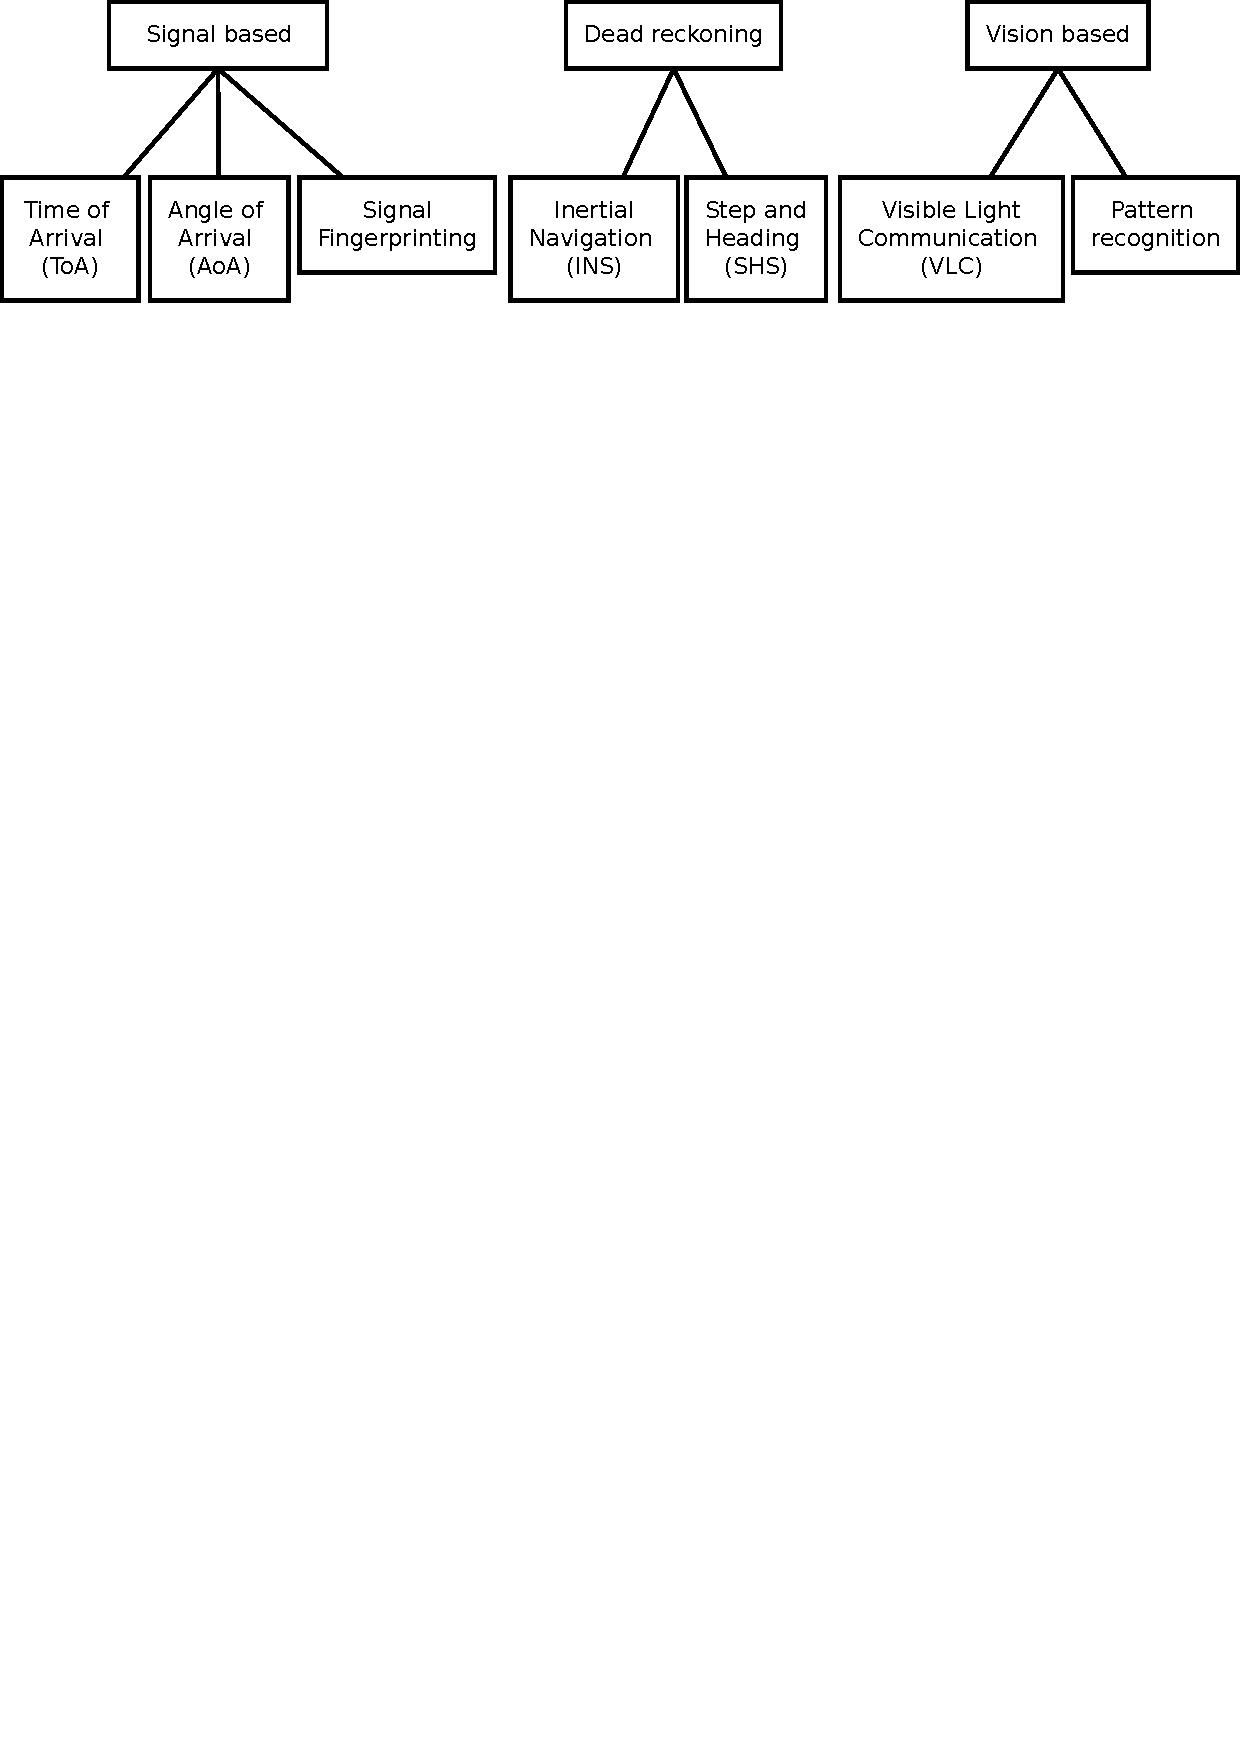
\includegraphics[width=\textwidth, trim={0 23cm 0 0},clip]{pictures/smartphone_localization_approaches.pdf}
\centering
\caption{Position finding approaches classification for smartphones.\cite{inertial_navi_velocity_model}}
\label{fig:smartphone_localization_approaches}
\end{figure}

Smartphone based indoor positioning approaches can be classified as shown on figure \ref{fig:smartphone_localization_approaches}. Signal processing is one of the most common used technique for positioning in mobile devices. They are equiped with radio transceivers that works on different frequencies and in different technologies when each of them are characterized with physical parameters that can be measured by the device and reuse for positioning purpose. More sophisticated signal solutions include techniques that provides additional data that can be used for positioning purpose like in case of Global Navigation Sattelite Systems. Dead reckoning approach comes from the possibilty of measuring the physical state of the handheld device by a set of incorporated sensors such as accelerometer or gyroscpe. Vision based solutions take an advantage from having camera being mounted on the device in order to run pattern recognition algorithms that can map acquired image to the position.

In this chapter there are revieved successful approaches for indoor positioning including hardware devices and infrastructure related system architectures and algorithmic approaches that are suitable for smarpthone devices.




TODO:
\begin{itemize}
	\item Advantages and disadvantages of solutions
	\item How the solutions fulfil given criteria (ex. how accurate given solution can be)
	\item Inertial navi system
\end{itemize}




With respect of the necessity of data distribution accross the positioning system there are avilable different solution architectures. Approaches can be categorised in a following way:
\begin{itemize}
	\item server -- client: positioning system infrastructure is capable for estimating the position of the system user. End user can fetch information about it's position from the server.
	\item client -- server: user of the system estimate his position himself and provide positioning information to the server,
	\item WSN and IoT approaches: user is treated as an extension of the positioning system infrastructure where infrastructure consists of a set of interconnected nodes that acquires the positioning related data and passes it through to the sink node while the user can listen to passing messages and interpret them,
	\item Peer-to-Peer: where user acquires available envioronmental data and passes it to the next user in range.
	%[Felix C. P. Hui, Henry C. B. Chan, and S. H. Fung. RFID-based Location Tracking System Using a Peer-to-Peer Network Architecture[J]. Lecture Notes in Engineering & Computer Science, 2014,2209(1):135-140.]
	%\item With respect of where environment layout model is stored (related - GIS systems; GeoSoft, Vulcan, MineSight, SURPAC Range, or Mining Visualization System (MVS))
\end{itemize}


\section{Wireless communication technology based solutions}
%Known solutions analysis (against defined criteria)

Wireless communication technologies are used for positioning purposes because of the fact that use electromagnetic waves which parameters are easily measureable, are open for extensions and suitable for hazardous and changing envioronments and finally they work without wires which can be broken during the works inside the underground installation. Another advatange is the low price of wireless communication modules and the wide application of various wireless communication technologies in computers and mobile devices such as smartphones.

This section introduces existing solutions for position finding that base on the wirreless technologies.

Commonly used techonologies for solving the problem of position finding in indoor environments are\cite{positioning_tests}:
\begin{itemize}
	\item Bluetooth Low Energy,
	\item ZigBee,
	\item WiFi,
	\item Ultra-wideband (UWB).
\end{itemize}

Bluetooth, ZigBee and WiFi technologies are the common technologies used in Received Signal Strength (RSS) based positioning techniques.

\subsection{Signal strength analysis and fingerprinting techniques} % (fold)
\label{sub:wifi_fingerprinting}

This section explains ideas behind Received Signal Strength analysis and fingerprinting techniches used for position finding solutions. Ideas are explained on example of WiFi wireless communication technology.

WiFi network infrastructure is a one of the available solutions that can be used as a source of information about current position of the device. The basic solution for positioning with use of this technology is about recognising wireless lan network access points by thier SSID or physical address of network cards \cite{WLAN_fingerprinting}. As there exists working position finding solution that base on that technology the accuracy of the solution is about 100-300 meters \cite{thesis_tablet_positioning}.

What is specific for radio waves attenuation at 2,4 GHz frequency is that their signal is present from relative large distances in mine in compare to the same devices signal range in the open space environment. What is also characteristic is that the signal strength, after its peak close to the WiFi transceiver antenna its going to stabilize in distance about 10m from source and then the signal strength is residing on similiar level up to distance arround 300 meters from its source when it goes down \cite{Thesis_CM}.

\begin{figure}[!htbp]
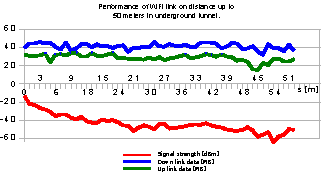
\includegraphics[width=\textwidth]{pictures/wifi_link_short.pdf}
\centering
\caption{Wireless lan throughput and signal strength with respect of distance from the signal source (wireless access point) \cite{Thesis_CM}. }
\label{fig:wifi_link_short}
\end{figure}


On figure \ref{fig:wifi_link_short} it is presented how wireless lan link parameters differs with respect of distance between client device and the network access point. Measures presented there are taken from 0 up to 50 meters from signal source. In case of this chart there were presented uplink and downlink throughput measured by amount of data gathered on each testing probe taken each meter distance from the signal source and the related signal strength expressed in dBm units. Values presented on chart are medians of all gathered values and factors for given distance. Test was caried out in straight underground tunnel in the biggest coal mine in Slovenia: Premogovnik Velenje. Connection throughtput between client and server remains nearly the same for distances in range from 0 up to 50 meters. Signal strength is presented in logarithimc unit dBm. Signal strength falls significantly in first 10 meters from 0 to -40 dBm. After distance of 10 meteres value of signal strength is ranged in between -40 and -50 dBm with small and not regular diviations. After 45 meters from source the value drops slightly bellow -50 dBm.

\begin{figure}[!htbp]
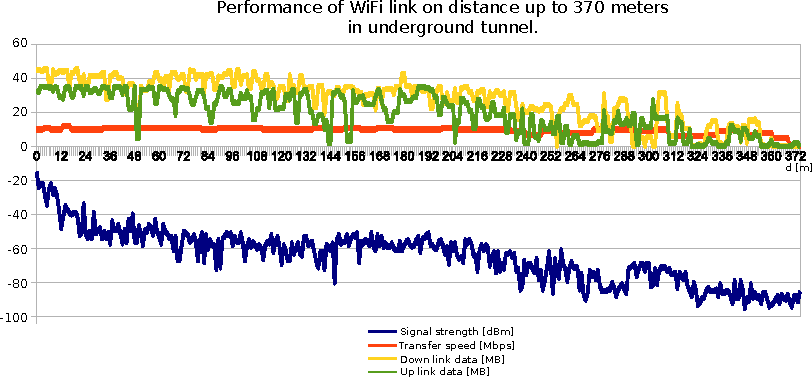
\includegraphics[width=\textwidth]{pictures/wifi_link_long.pdf}
\centering
\caption{Wireless lan range \cite{Thesis_CM}. }
\label{fig:wifi_link_long}
\end{figure}

Figure \ref{fig:wifi_link_long} presents tests results performed on longer distance till connvectivity was not possible due to too low signal strength. On distances from 50 up to 240 meters parameters of link are similiar. Down link data remains at 40 MB and at 38 after 140 meters with drops to 20 MB. Up link data measurments are more unstable than in case of down link in therms of drops in delivered amount of data, but trend seems to be steady on range from 50 till 220 meters from access point. Then both data uplink and down link drops by 10 MB.  Speed of data transfer between access point and client device remain similiar from very beggining till distance around 370 where signal is not enogh to conduct connection. Signal strength is characteristic only for first 10 meters from signal source. Then signal strength oscilates between -40 and -60 dBm on distances 10 -- 50 meters, between -50 and -80 dBm on distances 50 -- 240 meters, between -60 and -90 on distances 240 -- 320 meres and between -80 and -90 on longer distances. Following data does not represent any straight forward solution to adjust positioniong information to make positioning more precise and accurate. Only on distances close to the signal source it is possible to estimate more precise position while signal strength values differ significantly from the values that occures on the rest of distances. There can be identified following range zones with respect of WiFi signal behaviour \cite{Thesis_CM}:
\begin{enumerate}
	\item near field zone: 0 -- 40m distance from signal source where wave attenuation curve is similiar to that in free field distribution,
	\item coverage zone: 40 -- 200m distance from signals source where can be identified symptoms of waveguide propagation and signal strength remain to be arround -50 dBm,
	\item monitoring zone: distances since 200m from signals source where signal starts to vary from -75 up to -85 dBm and becomes to be unusable for communication purpose but client and access point are visible for each other,
	\item out-of-range zone: where signal is too low and both client and access point are not visible for each other.
\end{enumerate}

One of the approaches for the Wireless LAN based positioniong system is to assume that given client is present in given area of underground installation if it is in coverage zone of one of Wireless LAN access point. Client can be registered by access point software and followed until he leave coverage zone. As the coverage zone is about 200 meter distance from access point then total accuracy of this solution is about 400 meters. Second approach assume positioning accuracy improvment by signal strength interpretation and recognistion if client is in near field zone. This approach is easy to be implemented as signal strength values in near field zone differs from values from the rest of zones. Such solutions are implemented in mines in Germany \cite{Thesis_CM} and in Swedish Boliden's mines \cite{thesis_tablet_positioning}.


%TODO - wlan and AoA; wlan and ...???
%TODO - fingerprinting; There is known concept of recognising position in mine by informations distributed by


% subsection wifi_fingerprinting (end)

\subsection{Positioning with Beacons and Bluetooth technology} % (fold)
\label{sec:positioning_with_beacons_and_bluetooth_technology}

Beacons are transmitters that use Bluetooth low energy technology in order to send out small set of informations. They are designed to be small and energy efficient in order to allow them to be independent from the external power source. The main application of beacons are indoor positioning systems while beacons can be treated as a set of reference points building the static infrastructe of landmarks where the position is a funtion of received signal strength from beacons by the user. Beacons can be also attached to the non static objects or even user can emmit beacon information. Then the responsibility of position estimation lies on the infrastructure that gathers the signals.

Common way of estimating the position is taking into account the measure of received signal strength from the beacon transmitter called RSSI (received signal strength indicator). RSSI denotes the power of received radio signal measured in dBm (decibel-miliwatts). The measure is actually the raw value that express the powerd inducted on the receivers antenna as a result of transmission. None additional sensors are required to take that measure. Value is available on most of wireless technologies as a part of diagnotic report serving as indicator how good the connection is. The higher the RSSI value then the higher the signal strength so transmitter is closer to the receiver. Such relation between the RSSI value and the distance is known under a various of models that tries to describe the propagation of electromagnetic radio waves with use of some statisic and probabilitic distribution \cite{RSSI_path_loss_prediction_model}. Such models are needed because of calculus complexity while using actual physical model of the phenomena. In order to perform physical calculus there is need detailed description of the envioronment including every element that may influance the radio wave propagation. Calculus could include d'Alembert equation for signal power density on limited space which requires 6 variables concerning distance and time in 3 axis. Calculus should take into account presence of radio wave diffractions and attenuations on materials present in the indoor envioronment. As the propagation space is not ideal and the amount of elements influences the propagation is large such calculations are not being performed.

Example of statisically obtained model that descibes relation between received signal strength is \textit{Log-distance path loss model}:

\begin{equation}
\label{eq:log-distance-model}
	RSSI = -10 n \log_{10} (\frac{d}{d_0}) + A_0
\end{equation}



where $ d $ is the distance between the receiver and transmitter, $A_0$ is a reference RSSI value measured at $d_0$ distance from the transmitter, $n$ is the signal propagation exponent. Taking the measure of RSSI ($A_0$) at a distance of one meter from the signal source ($d_0 = 1$) simplifies the equation. That is the common practise which was even implemented into iBeacon protocol developed by Apple company by attaching additional information about reference $A_0$ RSSI value into the broadcast message of the beacon.

\textit{Log-distance path loss model} states that the only variable that influence the RSSI value is the distance from the source. Such model has to treaten as a rough distance estimation as RSSI is not a stable measure. Bluetooth technology operates on a 2,4GHz frequency which means that the wavelength of the signal is equal to 12,5 cm. Such short wavelength is prone to distrortion such as multi-path reflections where signal bounce against objects and material attenuation what makes the resultant measures noisy.

Bluetooth technology was developed and is maintened by the Bluetooth Special Interest Group (Bluetooth SIG) which is the standard organisation capable for licensing the Bluetooth technologies and trademarks to the manufacturers. Bluetooth technology operates on frequencies from 2,4GHz to 2,4835GHZ which was devided into into 80 channels. In order to adopt transmission channel to the current load on given frequencies, Bluetooth implement a mechanism called \textit{Adaptive Frequency Hopping} which allows to change channels being in use during the transmission without interrupting it. Subsequent Bluetooth technologies are aimed to ensure bigger data transfer, lower energy use and increase the transmission security. Since version 4.0 if Bluetooth standard there is availablable special protocol that is optimised for lower power consumption. This protocol is called \textit{Bluetooth Low Energy} while the whole Bluetooth 4.0 standard including classic and high speed protocols is called \textit{Bluetooth Smart}. Since 5.0 version of the standard the set of the protocols are called just \textit{Bluetooth 5}. Market is dominated with Beacons that use Bluetooth Low Energy protocol in version 4.0 that is why this paper focuses only on this version of protocol.

Bluetooth is as set of profiles. Each version of the technology contain definitions of profiles that are up to date to that version and optionally are reverse compatible with older ones. Each profile describe what communication protocols and data format it use. Protocols available for the profiles are also defined by the Bluetooth technology. Bluetooth Low Energy protocol use \textit{Generic Attribute Profile (GATT)} which is a set of services that can be used within the transaction between devices. Service is a name for collection of characteristics that express state of device. Bluetooth defines 59 services within the GATT such as TPS (Tx Power Service), IPS (Indoor Positioning Service) or HRS (Heart Rate Service). Services are idenfied by their UUID number which must be unique. Despite the defined service, there is a possibility to create own services. Characteristics are defined with given format type, properties and security permissions. There are available such format types as signed or unsigned integer ranging between 1 and 8 bytes, float, string or a structure. Allowed properties of the characteristics describe if the value within the characterisic can be readed (read property), changed (write property), required acknowledgement (indicate property) or being in use just for notification purposes (notify property). There is possibility to add custom properties as well. Security persmissions part of the characteristic definition are about definining if given property can be executed with or without an authentication. For example Measurement Interval characteristic of the Health Thermometer Service is defined with Read, Indicate and Write properties and security permissions stating that there is not required any authentication for reading but it is needed for writing.

Broadcast messages are way how Bluetooth Low Energy devices communicate with them selves. It is called \textit{advertisment mode}. In order to distinguish types of those messages (aka advertisement frames) they are different frame formats being in use. On the market of Beacons there are two major protocols that defines Beacons devices behavior, including broadcast frame format. The first -- \textit{iBeacon} -- was developed by Apple and the second -- \textit{Eddystone} -- was developed by Google. Those broadcast messages formats are the basis for creating "Ranges" definitions. Usage of ranges are explained further in section \ref{subs:smartphone_abilities_and_limitations}. In case of \textit{iBeacon}, advertisement frame consists of 29 bytes. First 9 bytes are constant preamble, defined by the \textit{iBeacon} protocol. First 3 bytes are standard Bluetooth Low Energy Flags. Next 6 bytes consists of type definition of the packet (in this case it is a \textit{Custom Manufacturer Packet}),  manufacturer ID (constant value that represents Apple company), subtype that indicates \textit{iBeacon} compatible device and number of bytes that are attached to the \textit{iBeacon} advertisement frame which is a constant number of 21 bytes.  \textit{iBeacon} specific data consists of \textit{Proximity UUID} field which must be unique accross different users, \textit{Major} and \textit{Minor} fields that gives the user possibility to differentiate Beacons that he own and the \textit{Signal Power} field which denotes received signal strength observed at distance of 1 m from the Beacon transmitter. \textit{Signal Power} value is commonly used to compute distance between receiver and transmitter using the \textit{Log-distance path loss model}. Then \textit{Signal Power} is assumed to be value of $A_0$ variable within equation \ref{eq:log-distance-model}, where the $d_0 = 1$. That is why the model can be simplified and distance can cumputed quickly just after receiving the advertisement frame by issuing the following equation:

\begin{equation}
	d = 10^{\frac{RSSI-A_0}{-10n}}
\end{equation}

$RSSI$ is a measure obtained during receiving process and $n$ is a constance.

\textit{Eddystone} protocol introduce three types of advertisement frames. They differ from \textit{iBeacon} by introducing seperate frame types for
\begin{itemize}
	\item passing encrypted identification data,
	\item passing information about Beacon state, aka telemetric frame,
	\item passing address of a web site related to the Beacon.
\end{itemize}

There are available general concepts for positioning systems based on Bluetooth technology dedicated for underground environment\cite{article_inertial_active_beacons_calculus_kalman}\cite{positioning_tests}\cite{thesis_tablet_positioning}, but their concepts were not verified in real environment or are not applicable to be used by smartphones.

% section positioning_with_beacons_and_bluetooth_technology (end)


\subsection{WSN based position finding systems} % (fold)
\label{sub:wsn_based_position_finding_systems}

There are proposals of position finiding and tracking systems based internet of things (IOT) soultions \cite{WSN_tracking, WSN_monitoring}. The idea is to create means of wireless communication to locate miners during their daily basis. It is proposed to create a network of wireless nodes (WSN) that read signal from tag devices (RFID) carried by miners and transfer it through nodes network to sink nodes that are directly connected to the mine core data transfer installation such as industrial Ethernet. Miners position data is sent to acquisition server. Intermediate and nodes are directly connected one or more nodes laying in the range of their wireless communication module. They form together ad hoc, multi-hop, self-organizing network of nodes that is able to transfer data, reorganise its structure in case of mailfunction of one of the nodes and allow to configure nodes remotely due to the implemented wireless communication technology and dedicated routing protocol. Network of nodes can be easily expanded by adding new nodes. Due to the fact that communication is wireless, nodes can be placed also in danger or new areas where wired network devices are not allowed or the related infrastructure doesn't exists.


WSN and RFID based positioning system is designed to serve such functionalities as querying miner information, locating miner, tracking miner and managing tag and reader. It is proposed to use this system along with simillary implemented monitoring system that measure safety parameters in mine \cite{WSN_monitoring}. This positioning system is dedicated to used by production monitoring, production scheduling and emergency rescue mine departments located on surface. Bigger precision can achived by adding more nodes into the network. Technology that is used for wireless communication between WSN nodes can be a Bluetooth Low Energy, ZigBee (IEEE 802.15.4 based) or WiFi (IEEE 802.11). ZigBee technology is the most popular in WSN's as it supports variety of communication modes, contain out-of-box solutions for network topology management and support low energy solutions like sleep modes \cite{ZigBee_applications}. ZigBee protocol which is dedicated for ZigBee technology uses energy and computational efficient solutions for data collision avoidance which includes CSMA/CA techniques and time division concept \cite{WSN_monitoring, ZigBee_desc}. There are three main topologies forced by ZigBee technology that can be used in the WSN network: star topology, tree topology and mesh topology. Star topology limits the network to have all nodes directly connected to sink. Tree topology enables multihop functionalities but litmits network flexibility in therms of adopting routes in case of filure (doesn't support redundant connections between nodes). Mesh topology requires to store routing tables in each node but provides means of redundancy in therms of routing what makes the WSN network reliable and fault resistant \cite{ZigBee_desc}. The WSN positioning network proposal base on ZigBee technology and it's mesh topology. Placement of WSN nodes should guarantee signal coverage of RFID readers modules build into nodes. On order to achive that there are proposed variety of topologies that can be used on site during network installation. On image \ref{fig:wsn_topology} it is presented the network topology proposal that introduces intermediate nodes -- routing nodes -- that gather information from sensor nodes and transfer it through network of routing nodes to server via sink node \cite{WSN_monitoring}.  Due to the fact that WSN nodes are limited in energy supply, systems that base on that technology needs to be designed with aware of energy management and fault management. Idea of routing nodes deployment along the tunnel in two simmetrical lines comes from the need of link redundancy between nodes. Thanks to that even if some of routing nodes are down the information from sensors can be passed out through the other routing nodes that are in range. In order to limit power consumtion of reader nodes they were designed as Reduced Function Devices (RFD). These nodes do not take a part within information passing process. Reader nodes are designed only in purpose of reading signals from RFID tags and to send the information to the nearest routing node. In order to achive that the information will be sent only to the nearest reouting node there is performed initial configuration process that involve both reader nodes and route nodes in its signal propagation range. The process is such: reader node send the testing signal to all of the nodes. Nodes that were able to reiceve the signal, send responce with value of Received Signal Strength Indication (RSSI). Reader node limit its sending power according to the responces. Thanks to it power consumtion of reader node and interference with neighboring nodes are reduced.
%WHAT IS THE PRECISION? HOW CAN BE APPLIED INTO MOBILE PHONE (TARGET)? WHAT IS NODES POWER SUPPLY?

\begin{figure}[!htbp]
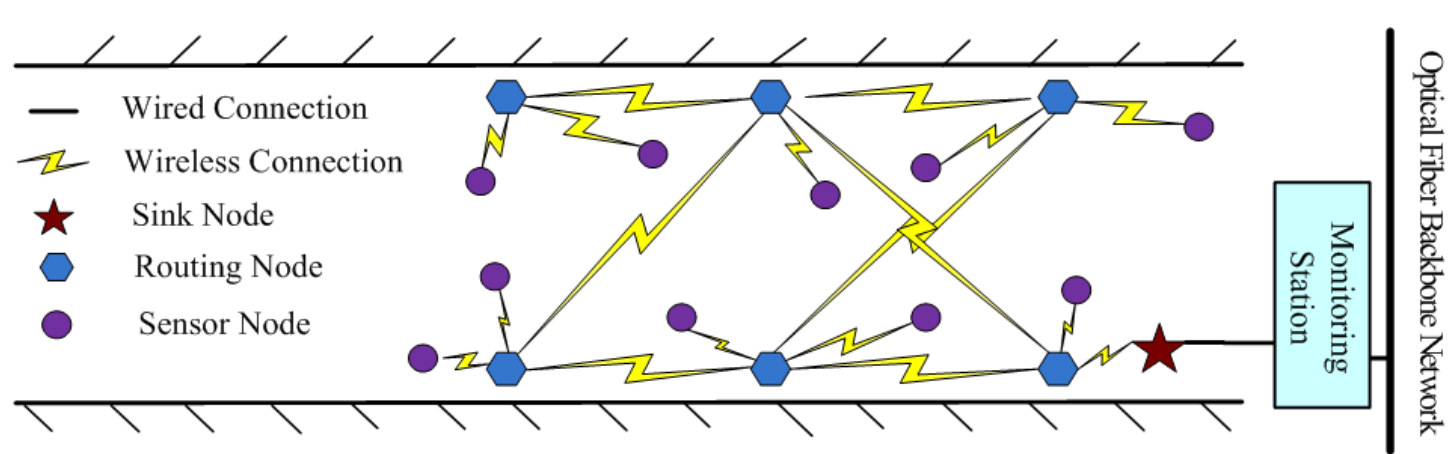
\includegraphics[width=\textwidth]{pictures/wsn_topology.png}
\centering
\caption{Wireless Network Sensor topology in underground corridor example \cite{WSN_monitoring}. }
\label{fig:wsn_topology}
\end{figure}

%WSN routing and topology
Network of wireless connected nodes needs be designed with respect of its maintability. There is need to assume that some nodes may fail during their operation. As the network consits of many nodes, where the number of nodes can be changed during thier operation, there is need to implement actions that will allow them to organize their topology automatically. Even if particural nodes will fail, the rest of nodes should be able to work and maintain communication with remote services. It is the role of implemented routing protocol. There are available solutions that allow network to adapt quickly to the changing environment \cite{WSN_collective}, but in case of statically placed network elements the environment is not changing havily. As it is in common practise, routing nodes stores information about nodes that are used for network purposes in the routing tables. Rounting tables are created with the manner that there are promoted link to nodes that ensure the lowest cost (distance) of packet travel from given node to the sink node. Routing table can have many entries. In case of topology for underground installation there are suggested 3 entries: parent route, minimum route, backup route \cite{WSN_monitoring}. Parent route points to the parent node, minimum route points to the best node in therms of the most energy efficient way to the sink node and backup node that points to the second to the best routing node. Each entry consists of elements such as: number of hops (routing nodes from itself to the sink node), value expressing quality of link of the last communication, flag that describe the role of the entry (parent, minimum, backup route). Routing tables and interconnections between nodes are created during network installation process. The idea is that the sink node that is directly connected to external communication medium creates at first 1-node WSN. Rest of nodes organize themselves in manner that nodes broadcasts their physical and network adresses. Basing on information gathered during installation they are able to determine their position in the network, obtain network address, assign routing table entries and obtain hop number. The network topology can be build up and maintain after WSN installation process \cite{ZigBee_applications}. Nodes are able to pass information to sink node that contains it's routing tables. Thanks to that sink node is able to recreate network topology and then pass the information to the external server. In order to maintain the network there are implemented status messages that contain information about changes in nodes routing tables. They are usually pass through WSN along with data from periodic sensor readings.

%WSN power management
Nodes are equiped with batteries that makes them independent from external power source. In order to save the energy and in order to prolong device live on the battery nodes works in energy efficient modes. In these modes nodes are turned into sleep for certain time. They woke up in order to perform tag readings and transfer the data to the external resources. In order to synchronize their operation, in each cycle the sink node broadcasts the initial message which is used to synchronize all of attached nodes. Power level of nodes batteries are monitored. Nodes can send information about their power level as a repsponce for appropriate request. There can be implemented special routines inside node that can cause sending the information about the low battery level in emergency mode, without any request from the sink node.

%WSN Location management
The crucial for the positioning system is to determine accurately exact position of given reader node inside the underground installations. Without information about readers placement positioning data obtained from them are not usefull. Solution for this problem in WSN positioning systems are solved by manual configuration. Each node have it's own identification number that is a part of it's initial configuration. This number is atteched into their housing also so given nodes can be identified directly during the installation or maintenance work in tunnel. As nodes deployment is regular it is assument in advance what will be the position of the node within the tunnel. In case of sudden failure of some node it is possible to determinate which of the node is broken by it's ID information, and check were the node is placed. WSN network should have possibility to report failure of its nodes. That is why WSN positioning systems are equiped with failure detection and reporting mechanism. Parent nodes like routing nodes against reader nodes, checks if child nodes responds to the requests. In case of having no response from given node for a given amount of subsequent requests then parent node issue status request command to the child node and wait given amount of time. If child node give an answer then it is assumed that the given child node is working correctly. In case of no response from child node, the parent node send information about failure to external service. As the readers nodes are connected stright to the parent node with no routing options then different policy for borken parent node must be applied. If the child node does not reiceve acknowledgement (ACK) frame from it's parent given amount of times then the node increase it's sending power and retrainsmits it's data again. If there is no result of increasing the power then node goes into network setup mode and scan channel to rejoin the network.

%General solution Architecture
Positioning algorithm in WSN positioning system base on mine layout and assume fixed position of nodes. Information about mine layout and nodes position wihin mine is stored in database on server above ground. Data transferred from nodes into acquisition server is a combination of three values: ID of a node, ID of acquried RFID tag in range of RFID reader module of that node, signal power of this RFID tag, and timestamp. Data is being stored in simplified relational database. This positioning system uses algorithm for finding exact position of RFID tag in dwo diamensional space (x, y). In order to do that algorithm search in database for 3 nodes that acquired given tag sinal with the biggest power. Then it uses simple free space electromagnetic waves propagation model \eqref{eq:prop} to compute distance between node and tag.

\begin{equation}
\label{eq:prop}
P_{ri}=\frac{P_t \cdot G_t \cdot G_{ri} \cdot \lambda^2}{4\pi D_i^2}
\end{equation}

Parameters $P_t$ (signal power generated by tag), $G_t$ (tag antenna gain), $G_{ri}$ (node reader antenna gain) and $\lambda$ (electromagnetic wave length) are constant and known. Parameter ${P_{ri}}$ (received signal power on reader's input) is the only variable in the equation that is needed to compute distance from tag to reader. Maximum likelihood estimation method that base on data from three nodes and thier values of reiceved signal power from given tag produces relative position of given tag in (x, y) coordinates. Suggested implementation \cite{WSN_tracking} assume that nodes look for RFID nodes each 10 minutes.
% subsubsection wsn_based_positioning_finding_systems (end)

%drawback of WSN - simplified assumtion about propagation in underground corridors because of wave diffractions on it's walls; - not needed precision of two diamensional space; assumption about RFID tag range (WHAT IS THE RANGE OF RFID). In order to fulfill assumption there is need to put WSN nodes close to each other which higher the costs; - Limited lifetime
%advantages of WSN - wireless nodes with rfid reader modules are cheaper than wired ones (in the same price we can install more nodes)

\section{Other solutions} % (fold)
\label{sec:other_solutions}

Position finding solutions use also other means of sensing the environmental parameters than those making use of wireless communication technologies modules. Potential positioning approaches for underground installations include:
\begin{itemize}
	\item Passive RFID,
	\item Inertial Measurement Unit (IMU),
	\item Magnetic Field strength pattern matching,
	\item Very-low frequency (VLF) electromagnetic waves,
	\item Visible Light Communication (VLC).
\end{itemize}

In the underground installations image processing (aka \textit{computer vision}) solutions for positioning systems and solutions concerning pattern recognition (like \textit{activity-based navigation} \cite{article_visual_points_AR_navi}) are not investigated due to the poor visibility, lack of patterns that can identify current position admittedly as well as the fact that painted signs are quicly covered by the dust making them difficult to read.


% section other_solutions (end)
\subsection{Radio Frequency Identification tags} % (fold)
\label{sub:rfid_tags}

RFID technology make use of electromagnetic field phenomena that allows to transfer information to reader from special component, RFID tag. Passive RFID tags are powered by readers though electromagnetic field; they do not use batteries or wired external supply. In order to acquire information from tag readers have to propagate electromagnetic waves. Tags cumulates power from electromagnetic field in capacitor. When tag have enough power then it transmits the response with tag's data to the reader and goes to sleep for a given time. Reader get signal from tag and perform filtering and decoding operations on it in order to get tag's data. There are also available variants of active RFID tags wich use it's own power supply.

RFID technology is used in underground installations in certain locations to serve as check points. In this manner are monitored underground trains or dispatch of materials is being monitored. Passive RFID modules are installed on containers or mobile machines like trains. Those modules can be read by passive RFID readers that are connected to the mine network via dedicated control unit like Mining Infrastructure Computer \cite{Thesis_CM}. Control unit is responsible for RFID reader configuration and translation of its readings into standarized positioning information format. It also supplement data from RFID reader with its identificator or coordinates which express position of a reader on mine model. RFID can operate at 868MHz band. RFID with 8dBi antenna is able to detect RFID passive tags at range of up to 3 meters.

%WHAT IS THE RANGE? HOW MANY ENERGY MUST BE USED TO GET THE DATA FROM RFID?
% subsection rfid_tags (end)


\subsection{Visible Light Based positioning system} % (fold)
\label{sub:visible_light_based_positioning_system}


Visible Light Communication (VLC) is a method for using visible spectrum of electromagnetic waves for exchanging the data. Communication system requires source of the light and light sensor which is able to detect light modulations. In case of simple signal modulations like PWM, camera of a smartphone -- complementary
metal-oxide-semiconductor (CMOS) image sensor can be also used effectively for receiving modulated data. Source of light in these systems are LEDs. LED is a semiconductor device that can be easily controllable by logical unit. LEDs are characterised with low latency during changing their state from on to off and vice versa. It was masured that rising and falling edges during switching the state are about $4 \micro s$ long \cite{visible_light_positioning_epsilon}. Usage of these kind of medium for wireless communication purposes was already standarized by IEEE 802.15.7.

Advantage of VLC is that LED technology is commonly used as a light source in buildings and outdoors. If LED will be prepared for its unique ID transmission or transmission of its position expressed in 3D diamensions then the VLC system can be used as a positioning system with static anchors working as a beacons. Such positioning systems are called visible light positioning systems (VLP). All of them consists from three main components:
\begin{itemize}
	\item light beaconing, which assigns special factor to the light source making it unique and distinguishable among others for the receiver,
	\item distance estimation, which can be obtained by taking the measure of a received signal strength and a signal strength based distance model,
	\item localization, which provides actual information about the position of a receiver. This can be obtain with use of trilateration, multirateration techniques or methods like angle of arrival.
\end{itemize}

Simple light sensor is the source of the received light information that is not aware about the light source relative position or angle but gives only the signal strength measure. CMOS sensor provide more information about acquired image beacase output consist of a two-dimentional map of sinal strengths. In this case it is possible to make use of an optic phisical laws in order to get relative position of a beacon. When there are three or more light transmitters available then it is possible to obtain receiver position in 3-D coordinates.

\begin{figure}[!htbp]
 % trim={<left> <lower> <right> <upper>}
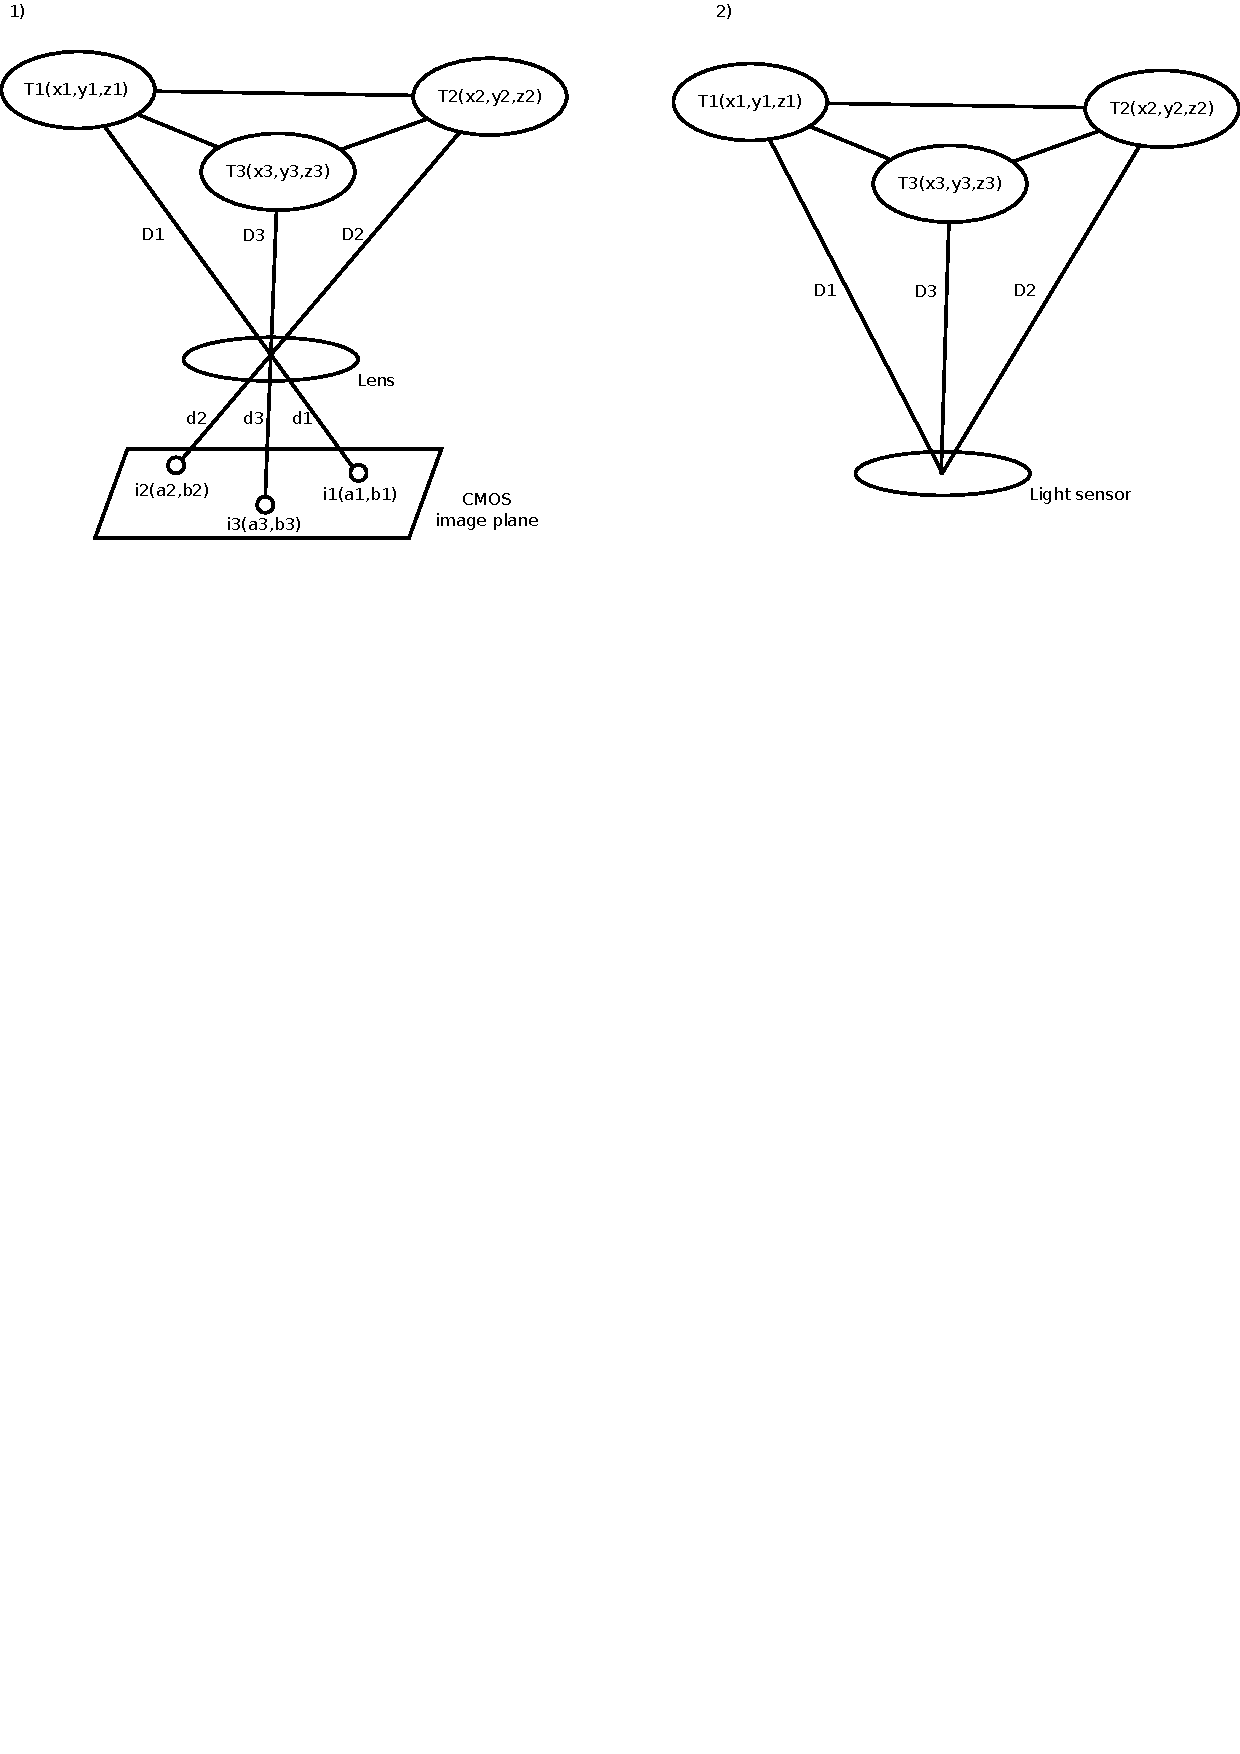
\includegraphics[width=\textwidth, trim={0 20cm 0 0},clip]{pictures/visible_positioning.pdf}
\centering
\caption{Visible Light Positioning system principles. Diagram 1) presents concept of positioning system that make use of CMOS sensor  \cite{visible_light_positioning}. Diagram 2) presents concept of positioning system that make use of simple received signal strength measures and related distance model \cite{visible_light_positioning_epsilon}.}
\label{fig:visible_positioning}
\end{figure}

There are investigated various modulation methods that tries to tackle with natural difficulties connected with visible light frequencies. Main of them are sun, ambient and fluoresecent light interferences with the carrier frequency and specular reflections \cite{visible_light_positioning}. As a modulation schemes there are being in use on-off keying, variable pulse-position modulation, color shift keying, binary frequency shift keying, channel hopping and pulse width modulation.
% subsection visible_light_based_positioning_system (end)

\section{Applicability of smartphones in position finding solutions} % (fold)
\label{sec:mobile_device_dedicated_positioning_systems}

Todays smartphone class mobile device contains set of sensorics that can be used as a base for interial positioning system. In underground oprations industry this idea is not the newest as there were tryies of this technology implementations inside handheld devices for people working underground with use of semiconductor based MEMS gyroscopes \cite{Thesis_CM}. Such devices were connected to the underground wireless network through access points which was responsible for transfering positioning information to the central systems above ground.

Smartphone class devices contains set of components that are treated as common in the industry. There is no strict definition what components should or should not the smartphone class mobile device contain as there is a strong competition in the market offering those devices in various configurations, shapes and fetures. This paper focus on devices that are compliant with Android operating system, especially version 7.0 which is currently (in the middle of 2018), the most popular operating system on the market. \cite{android7.0_cdd}. Android operating system forces hardware manufactures to equip devices with at least a minimal set of components needed for the system normal operation and give recommendations of optional components that are natively supported by the system\cite{android7.0_cdd}. In this section there will be investigated only those technologies that are available for the basic handheld mobile device with Android 7.0.

Smartphone class mobile devices are treated in the engeener industry as a powerfull tool set helping the workers with their maintenance work on site and as a handy platform for wide scale of businesss oriented applications for task management and reporting. Factors that attract potential users of such smartphone based solutions are mainly connected with the price of those devices, ease of use, well described and supported programming frameworks and IDE, ready to use libraries, solved main power management and security issues, ease of maintenance, modularity, scalability, support for the most popular data exchange technologies, ease of extending the functionality by adding the support for external, wireless equipment. Smartphones that are available in the market are also equiped with the sensorics that allow the users to detect, record and recognise the phisical movements or orientation changes. It extends the positioning functionality making it more robust and acurate\cite{article_Inertial-sensors-for-smartphones}.
% section mobile_device_dedicated_positioning_systems (end)

\subsection{Mobile device sensorics}

There is no limitation in extending smartphones with internal sensorics. Acording to the Android 7.0 Compatibility Definition Document\cite{android7.0_cdd} there is no such sensoric that must be mounted and implemented into the Android system in order to be compatible with the operating system. It is also stated that device can contain as many various sensorics as producer wish under condition of having a compliant software implementation that deals with the sensorics. Although Android compatibility definition recognise some of them and recommends to be installed on the device. There are also technical requirements given under the sensorics recommendation in case of presence of such on the device.

In sake of simplicity Android defines all of componentes providing external information to the device as sensors. Thus components such as GPS signal receiver or a processed and filtered sensor fusion outcome like in case of rotation vector (fusion of accelerometer and gyroscope data) are recognised as different kinds of sensors. Such abstract definition comes from the Sensor Stack which is the part of Android framework.

Sensorics mentioned in the compatibility definition are:
\begin{itemize}
 	\item Accelerometer,
	\item Magnetometer,
	\item GPS,
	\item Gyroscope,
	\item Barometer,
	\item Thermometer,
	\item Photometer,
	\item Proximity Sensor,
	\item Fingerprint Sensor,
	\item 6-DOF Pose Sensor.
 \end{itemize}

All of components listed above, except fignerprint sensor, thermometer and photometer, can be used within the position finding system in order to give extra information about current physical state of the device. Compatibility definition guarantee some quality parameters of sensorics mounted in the mobile phone.

3-axis accelerometer can be used to detect movement changes. It provides the information how big the change was in terms of force that the device was affected. Thanks to the information there can be identified if user made a step or to compute the speed of the user in some mean of transport like a robust car by computing integral function over time from detected acceleration. It is required from that sensor to raport events at least at 100 Hz frequency (recommended minimum frequency is 200 Hz), to detect forces in range of frefall case up to forces at value of four times the gravity (4g) or more on any axis, minimal outcome resolution is 12-bits (recommended minimum is 16-bits), should allow for online calibration and calibration parameters persistance, be temperature componsated and have a standard deviation no grated than $ 0.05 \frac{m}{s^2} $. Document defines also the maximum accepted amount of power that the sensor can consume during its operation - not more than 4 mW (recommended values are bellow 2 mW during the operation and bellow 0.5 mW when the device is in static condition).

3-axis magnetometer (aka compass) provides the data concerning detected values of the magnetic field. Data available from the operating system level are expressed are in micro-Tesla($\mu T$). Sensor must be able to measure between -900 $\mu T$ and +900 $\mu T$ on each axis before saturating with the resolution of 0.6 $\mu T$ (recommended 0.2 $\mu T$ or denser). Magnetometer have to compensate hard iron and soft iron effects where hard iron offset have to be less than 700 $\mu T$. That value forces the producers to place the sensor in as far from current-induced and magnet-induced magnetic fields like speaker. Sensor installation have to support online calibration and compensation methods and store the parameters in persistent memory. It is required from the magnetometer to report at minimum frequency of 10 Hz (recommended 50 Hz).

GPS/GNSS receiver is not required component for a smartphone with Android 7.0 operating system. If the sensor is mounted then it is required to match set of time, reliability and accuracy requirements like:
\begin{itemize}
	\item Fast time to first fix requirement - sensor have to determine its position within maximum 10 secods,
	\item Accuracy and responsiveness requirement - position have to be determined at least 95\% of the time under condition of acceleration up to $ 1 \frac{m}{s^2} $, within $ 20 m $ and speed $ 0.5 \frac{m}{s} $.
	\item Robustness requitement - have to be allowed to track at least 8 satelites from one constellation simultaneusely (recommended 24 GPS satelites at the time and one from other global positioning satelite system like Glonass, Beidou or Galileo).
\end{itemize}
It is assumed that the outcome of GPS "sensor" can be supported by the information issued from the Internet such as information about current sattelites position and can be based on some assised or predicted GPS technique.

Gyroscope is an angular change sensor. If installed on the device it must be able to measure up to 1000 degree change per second, report at frequency not less than 100 Hz (recommended 200 Hz), provide information of 12-bit resolution (16-bits are recommended), be self calibrating and compensating during its work, march variance requirement defined as $ 1e^7 \frac{rad^2}{s^2} $ per 1 Hz.

Barometer is an ambient air pressure sensor. It available is must report its measures at 5 Hz frequency, be temperature compensated and have "adequate precision" for altitude estimation.

Proximity sensor gives the proximity information of an object in the same direction as the screen. The required accuracy is at least 1-bit meaning that proximity sensor produces simple outcome that is interpreted as boolean value expressed state wether the user is close to the devices screen or not.

Pose sensor with 6 degrees of freedom (6-DOF) is an optional sensor that can be implemented in the Android compatible software. Sensor provides information about himself as part of the environment in perspective of end point of maniplator with 3 kinematic pairs, each with rotation possibilities. The method and related hardware is not discussed within the operating system compliance definition. The only rescriction stated to the sensor is that it have to be more accurate than rotation vector sensor. Basic implementation can make use of camera or depth sensor to compute the output value. Output is an quaretnion that express the rotation and a translation expressed in SI units. Sensor is used in virtual reality applications.

Android compliant definition strongly recommends the procudents to provide implementations of 'composite sensors' such as step detector, significant motion detector, gravity, linear acceleration, rotation vector. These measures are an efect of digital processing of data from single sensor like accelerometer in case of step detector or a sensor fusioning basing on multiple sensors like on megnetometer and gyroscope in case of rotation vector and accelerometer and magnetometer in case of geomagnetic rotation vector. The operating system recognise already filtered and processed data directly an outcome from an composite sensor which is actually a form of abstraction that hides the details of data processing.

Management of sensorics have to be implemented in a compliant manner in order to allow the operating system to interact with those sensorics. All of the sensor outcome are yet processed, normalized and expressed in a defined way like in case of an accelerometer and magnetometer where output is expressed within the "Android sensor coordinate system" format.


\subsection{Abilities and limitations of smartphone class mobile device in context of available positioning methods}
\label{subs:smartphone_abilities_and_limitations}

In sake of generalization this paper investigate case of regular consumer grade smartphone which are devices with a common setup compliant with Android 7.0 operating system. No specialized devices are taken into consideration.

Wireless technology is a common way for exchanging the data between the handheld mobile device and the envioronment. There are available GPS, Bluetooth, WiFi and terrestrial networks(GSM related) technologies. In case of underground each of these technologies has to be installed explicitely beacause bellow the ground none of these signals are available. GNSS (Global Navigation Satelite System) signal receiver is not usefull under the ground as there is no signal from sattelites available. There are tryies to make use of that technology by re-sending the acquired GNSS positioning data from sattelites in indoor environment by a set of transmitters that mimic sattelites \cite{GPS_retransmission} but it cannot be applied to the consumer grade smartphone as the Android applications have access to already processed pseudorange data into sattelite positions. Such solution is called Glonal Navigation Satelite System based indoor positioning system (GNSS-IPS)\cite{GPS_retransmission_differential}. Approach where transmitters places on ground fake sattelite signal is known as pseudolite. In case of indoor environment positioning data acquired from sattelites are drifted due to the fact of non-line-of-sight that is why position obtained indoor is called as pseudo-position. There are known tryies of using this approach in order to obtain positioning data but there is not known any sucessful implementation in underground environment.

Terrestrial networks, like GSM, can be also used as a source of positioning information but it requires some modification in order to shortcome problems with high variance of the signal. There is no possibility to do modification on that level to the Android software on devices available on the market nevertheless some prototype installations of extended terrestial network by positioning information were done and sucessful \cite{terrestrial_positioning}\cite{terrestrial_positioning_tdoa}.

Smartphone class devices are equiped with cameras. Images that captured by the cameras can be used for positioning purposes. There are known solutions that make use of visible light \cite{visible_light_positioning} that recognise source of light like LED which are called LED beacons and compute the position basing on the angle-of-arrival (AOA) algotithm.

Thanks to the presence of intertial sensors such as accelerometers and gyroscopes there are known implementations inertial navigation. Pedestrian Dead Recokoning (PDR) is based on the measures from the accelerometer which allows for step detection and an estimation of a step length \cite{inertial_navi_unaided} \cite{inertial_navi_pocket} \cite{inertial_navi_velocity_model}. Other approaches developes the recognition patterns that allows for distiction between transportation mean being in used. Such approaches were used for example in case of prototype navigation application in Chicago, London and Cologne subway \cite{inertial_navi_subway} or inertial navigation for bikes \cite{inertial_navi_bike}. There are known solutions for interial navigation improvment by aligning the outcome to the landmarks or map information \cite{positioning_tests}.

Positioning techniques that invole following devices are not useful or cannot be connected to the mobile devices:
\begin{itemize}
	\item laser scanner as long as it requires stable position for doing the environmental mapping and recognition and it needs to explicitly be extended to some wireless communication module,
	\item ultrasonic sensor as long as it requires stable position in order to measure signal travel time correctly and needs means of computational resources in order to process the raw data and send them thorugh some wireless connection to the mobile phone.
\end{itemize}

Smartphones provides support for Beacons - simple Bluetooth Low Energy devices. There are available libraries that allows monitoring of Bluetooth devices. There are available two modes for searching for Beacons: region monitoring and ranging. Region monitoring is an energy efficient way for searching for Beacons. It allows for long delays between consequent listening periods (like 10 seconds), turning receiver into sleep mode, and background service being active while the positioning application is turned off. In case where positioning application is turned off, the background service inform user that his smartphone found himself in the range of given Beacon region and run the positioning application. Such functionality is often implemented by shopping malls official applications allowing for location aware push-messages. Such advertising technique is called \textit{geofencing} \cite{beacon_rssi_analysis}. Region monitoring gives a rough information wether there is or there is not any Beacon device being in range. On the other hand, ranging gives details about all devices being in range with details such as RSSI, name, and other, protocol dependent data. Ranging use more receiver power as listening time is bigger (like 1 second) and there are smaller time intervals between consequent listening sessions (like 10 milliseconds). As it was explained in section \ref{sec:positioning_with_beacons_and_bluetooth_technology}, Beacons communicate their presence by sending broadcast messages called advertisement frames. With respect of the type of protocol being used there are available different formats for advertisement frames known as beacon layouts. Layout denotes the constraints that characterise given advertisement frame as well as variables and fields that are being included into frame.

TODO - describe each of pros
TODO - describe each of cons


\begin{itemize}
	\item Which of them will be useful to increase positioning accuracy
	\item Why mobile device is good for positioning purposes? What are the factors?
	\item What means of communication (ex. wireless) can be used in context of positioning system
	\item Battery limitations
	\item Sensitivity of receivers
\end{itemize}


\subsection{Position finding basing on localization system and mobile device model}

Localization system choise (system based on beacons)
\begin{itemize}
	\item  Motivation
	\item  Prototype system description
	\item  Mobile device - system interaction description
	\begin{itemize}
		\item  Method of detecting reference points description
		\item  What are the possibilities to improve positioning on your mobile device?
		\item  How could the process of installing a localisation system in a mine look like?
		\item  How the parameters of the environment (corridor height, corridor width, type of rock, type of corridor corridors, presence of other networks operating on similar frequencies (WiFi, GSM (harmonic frequencies)), others) affect reference point signal quality.
	\end{itemize}
\end{itemize}


\section{Solution requirements}
Positioning system as such have to match requirements related to the reliability and robustness, accuracy, power efficiency, installation and maintenance effort and safety. As the smartphone device is also a part of the solution then proposed positioning system must be able to interact with this device.

% Reliability and robustness
Provided positioning solution should allow users to make use of it within the ordinary works as well as in case of an accident. The minimum time that the positioning system should work without any external power supply is 72 hours. That value comes from a term of \textit{golden 72 hours} which relates to the period of time after the accident, after which survival rate decreases rapidly \cite{positioning_tests}. System should work also in case when part of it's infrastructure is not working properly like in case of an accident where some corridors can be destroyed including the positioning system infrastructure.

%Installation and maintenance
Ease of maintenance in terms of semi-automated methods for detecting the pitfails or failures and posibility to fix broken positioning infrastrucrture without necessity of involving specialised engineers should be matched. Such requirement can be met for example by simplicity of the positioning system infrastructure or automated configuration methods that makes the infrastructure self-organising itself. Infrastructure should be also scallable as underground installations are likely to be extended during the excavation process. Infrastructure should be open for software and internal modules updates and extensions of already mounted devices. That allows the positioning system to be further developed.

% Power efficiency
Power efficiency is an requirement that causes the system to be more likely independent from the on-site power supply. Infrastructure can have own power source and set of methods that limits power consumption of its devices. Infrastructure can be also extended by some power harvesting methods such as thermoelectric or piezoelectric generators.

% Smartphone
Smartphone must provide energy-efficient solution for exchanging the data with positioning system while there are no battery charging points in underground installations. Smartphone with positioning extension activated should be able to work at least for 8 hours and possibly 72 hours with a limited use of a positioning extension. 8 hours is the regular worker shift time in underground mines. Solution must be applicable for different models of smartphones.

% Usability
Solution must be easy to use for the user. In particular it should be integrated into the user smartphone in such a way that the user will not have to handle it in a specific way in order to use the positioning system. For example solution must be suited to work while the users smartphone is kept in his pocket as well as hold by the user in hand in front of him. Solution must be suited to provide positioning information when the user is not moving as well as he is walking. There should be assumed walking pace as $5 \frac{km}{h}$. Possibilities to adopt the solution to work with the higher speed of the user or, for example, users riding inside the vehicles are in plus.

% Accuracy
Solution must be able to provide positioning information in real time manner. Under assumption that user of the system will be walking inside underground installation, there is need to ensure position update frequency of at least one per second. Position of the users should be provided with maximum drift of 10 meters.

% Safety requirement
Safety purpose of position finding system is very important for many countries \cite{positioning_tests}. European Union encourages to search for a good solution for the miners localization, which, in one of the postulates of its set of recommendations for the coal and steel sector ('Personnel Tracking' task). There are solutions for underground localisation but they allows only to approximate miner's position (error can be range from 300 m (range of a single radio receiver) to the distance to the next transmitter).

Underground position finding system must be compatible with mobile devices of smartphone class. Special mobile devices that were prepared to work in bad conditions like in coal or salt mines differs mainly with their housing in compare their non-commercial, personal-use equivalents. This assumption limits the range of available technologies that can be used in order to provide means of communication between mobile device and the enviornment.

Position finding system bases on idea of interaction between mobile device and the undeground envioronment. In case of the nessesity of extension that enviornment by electionic devices that will provide positioning data or means of connection with mine network there is need to state that such devices must be safe. Safety regulations in this matter differs with respect of the type of underground installation, the regional, country, or even association of countries \cite{Thesis_CM}. The goal of this paper is not to provide solution that will be adjusted to each installation type or safety regulation, but to investigate possibilities and propose state of the art solution. As the enviornmental restrictions for devices and related infrastructure that can be needed for given solution there will be assumed general rules that are being in use in commercial tunneling \cite{Thesis_CM}.


Requirements summary stated for a positioning system and related infrastructure:
\begin{itemize}
	\item Reliability / robustness
	\begin{itemize}
		\item must be able to work wihout external supply for at least 72 hours,
		\item must be able to work even in case where part of infstratructure is not available.
	\end{itemize}
	\item Installation and maintenance
	\begin{itemize}
		\item semi-automated methods for monitoring the positioning system status,
		\item support for positioning infrastructure reperation by avoiding manual system reconfiguration,
		\item solution should be scallable in order to extend positioning system with the new corridors,
		\item infrastructure devices should be open for software and internal modules updates and extensions.
	\end{itemize}
	\item Power efficiency
	\begin{itemize}
		\item Possibly self powered.
	\end{itemize}
	\item Accuracy related
	\begin{itemize}
		\item responsiveness: position update with frequency least one per second,
		\item position error less or equal to 10m.
	\end{itemize}
	\item Smartphone related
	\begin{itemize}
		\item positioning system must be compliant with technologies supported by customer grade smartphone device,
		\item smartphone should be able to work continuously for the 8 hours with activated positioning module.
		\item recommended smartphone life time is 72 hours with limited power consumption and use of positioning module.
		\item solution applicable for different smartphone models.
	\end{itemize}
	\item Usability
	\begin{itemize}
		\item Solution must allow the user to be able to use the solution without forcing him to handle his smartphone in a special way.
		\item Suited for the walking man.
		\item inftrastructure components must be size suited to the proposed mounting placement,
	\end{itemize}
	\item Safety
	\begin{itemize}
		\item must be explosion proof and intrinsically safe,
		\item should be suited to the ingress protection (IP) standards,
		\item must have durable housing.
	\end{itemize}
\end{itemize}


% TODO
Requirements as the position of the mobile device will be determined by the environment model.

Define criteria that are the basis for position finding solutions comparison (existing or conceptual):
\begin{itemize}
	\item How to save a corridor model in computer memory
	\item wireless communication
	\item resistance to power outages and communications
	\item Do I need the ability to change configuration of reference points (configuration of devices that perform role of reference points)?
	\item What parameters can be read from the reference points (range, distance, ?)
	\item How long should the network work properly?
	\item How to detect irregularities in reference points?
	\item How to fix problems in reference points?
	\item What problems may occur with points of reference?
	\item If there are restrictions upon existing network topology (ex. in order to get access to servers located on surface)
	\item Can the mobile device be useful in case of lack of signal (GSM/Wi-Fi/BLE)?
	\item example: accuracy, durability, cost, maintability (energy, fault)
\end{itemize}

\chapter{Mobile device position finding algorithm}
* Algorithm that will make use of chosen localization system and mobile device internal sensors.

\section{Position finding requirements} % (fold)
\label{sec:position_finding_requirements}
\begin{itemize}
	\item Should repeat and answer requirements stated for localization system.
	\item example:
	\begin{itemize}
		\item Reading signal and its parameters from reference points;
		\item Identification of reference points
		\item Current location presentation on the environment model
	\end{itemize}
\end{itemize}


% section position_finding_requirements (end)

\section{Solution architecture} % (fold)
\label{sec:solution_architecture}

General solution architecture for the prototype positioning system is presented on the figure \ref{fig:architecture_general}. Solution consists of:
\begin{itemize}
	\item reference system installation based on beacon devices,
	\item smartphone device with Bluetooth receiver and inertial sensorics (at least accelerometer),
	\item application for smartphone that process and combines the data from the environment and internal sensorics.
\end{itemize}

It is assumed that reference points infractructure is mounted in a way that each beacon is denoted in configuration file consisting of a list of beacons with placement position assigned. It is possible to make application more robust and underground installation site undepentent while position information can be provided by reference points itselves. This proposal rely on already defined beacon positionis as this approach allows each end-user application to work as a maintenance tool that is able to detect problems of the infrastructure including beacon failures. Proposal system does not include such maintenance feature but it may be an addon into the next release.

\begin{figure}[!htbp]
 % trim={<left> <lower> <right> <upper>}
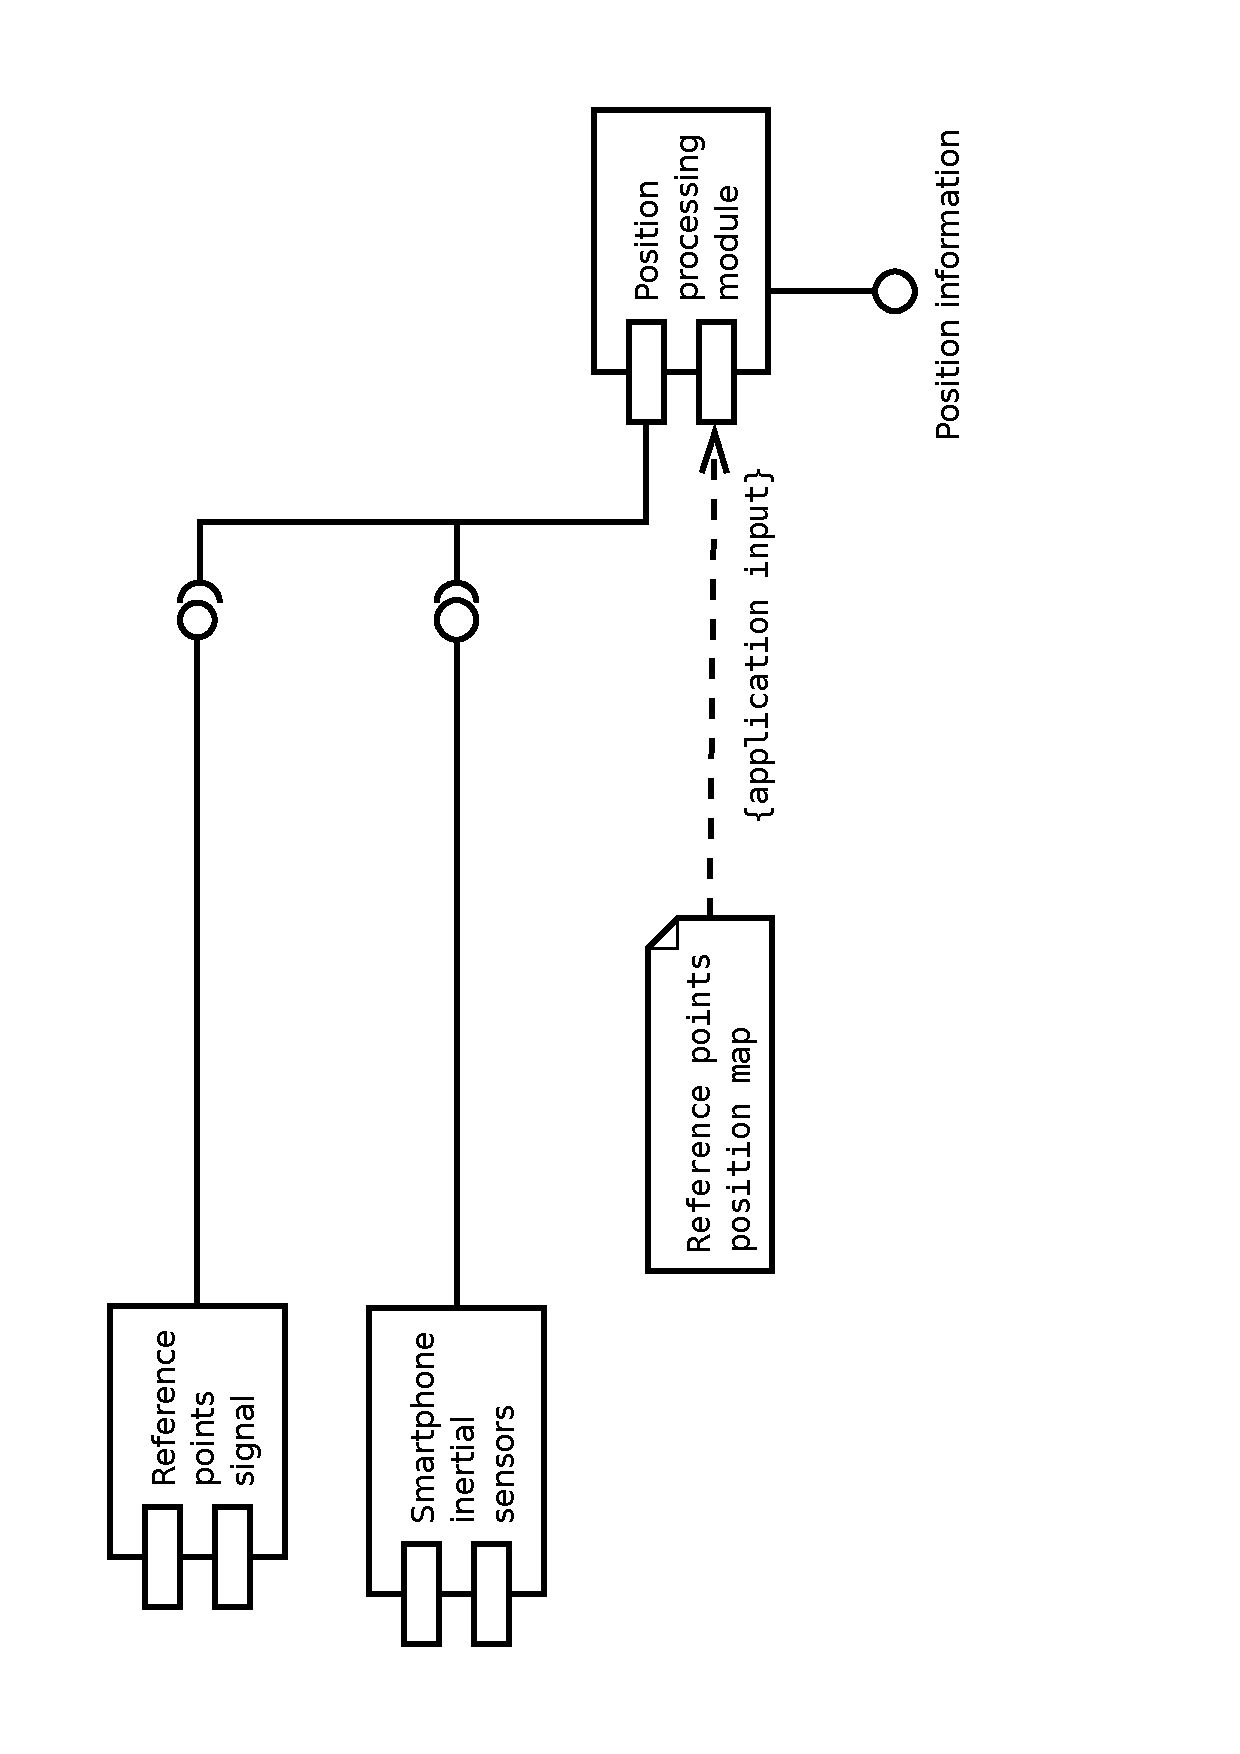
\includegraphics[height=\textwidth, angle=270, trim={0 0 4cm 0},clip]{pictures/architecture_general.pdf}
\centering
\caption{General solution architecture. Position processing module gathers data from smartphone sensorics, data and acquired signal parameters from reference points and serves current position as an output.}
\label{fig:architecture_general}
\end{figure}

The core positioning information is gathered from the reference points. They have constat position and they are the most corelated with the physical layout of underground installation. Having only this information it is possible to obtain positioning information as accurate as distance between subsequent beacons mounted on site. In order to make the position more accurate than in case of aligining the smartphone position to the position of the nearest beacon, there can be involved distance model that will allow for distance aproximation basing on the received signal strength value. As the signal strength in a tunnel varies havily there was no such model found or defined yet (refer to the section \ref{sec:positioning_with_beacons_and_bluetooth_technology}). Although there was proposed a solution that make positioning solution more accurate.

In order to maintain ability of determining the position by measuring received signal strength from beacons and provide long battery life of the beacon in the same time there were following beacon trasmission parameters assumed:
\begin{itemize}
	\item beacon will send his advertisement frame once per second,
	\item beacon will be set up with $-16 dBm$ transmitter power or equivalent that ensure beacon coverage of $20 m$ in underground environment,
	\item beacons will be placed in $10 m$ distances between each other,
	\item beacons which advertisement messages were received with more than $-85 dBm$ RSSI are assumed to be \textit{immediate} to the smartphone, those with more than $-95 dBm$ RSSi are assumed to be \textit{near} to the smartphone, rest are assumed to be placed \textit{far},
	\item if there was found at least one \textit{immediate} beacon then current smartphone position is assumed to be same as the beacon with the highest RSSI value.
	\item if there are two or more \textit{near}-placed beacons and if there was found similiar ($+/- 2 dBm$) RSSI values among them, the current smarthone position is assumed to be in a half way between beacons with these similiar RSSI values.
\end{itemize}

Due to the fact that received signal strength has significantly bigger values within the area of $0 m$ -- $2,5 m$ from the transmitter then this distance was classified as \textit{immediate}. RSSI values observed in \textit{immediate} range were bigger than $-85 dBm$. RSSI values lower than $-95 dBm$ are treated as a noise thus frames that were acquired with such RSSI value or lower are classified as \textit{far} and are placed in $20 m$ or more from the smartphone receiver. Signals with RSSI between $-85 dBm$ -- $-95 dBm$ are assumed that were sent by beacons which are classified as \textit{near}, placed in range $2,5 m$ -- $20 m$ from smartphone.

In proposed solution each beacon is placed in $10 m$ gaps. Each beacon is configured to cover distance of maximum $20 m$ but minimum of $10 m$. Such assumptions causes redundancy where in the perfect scenario user that is staying \textit{immediate} to the beacon is aqcuiring signals also from two other \textit{near} beacons. In case when one of the beacons is not working there is still possibility to align current user position to the place where faulty beacon is mounted. That is possible due to the assumption that if smartphone detect two beacons that are \textit{near} and received signal strength of their advertisement frames are similiar then smartphone is in the middle of the beacons. similiar signal strength means that the difference between each of them is less than $2 dBm$ what is equal to $1,25 m$ according to \textit{Log-distance path loss model}.

Output of the intertial sensorics can produce missleading position information. For example basing on the accelereometer data only it may turn out that the user have changed direction of the movement while he is still moving forward. It may effect with worsen the positioning information instead of making the position more accurate.

\begin{figure}[!htbp]
 % trim={<left> <lower> <right> <upper>}
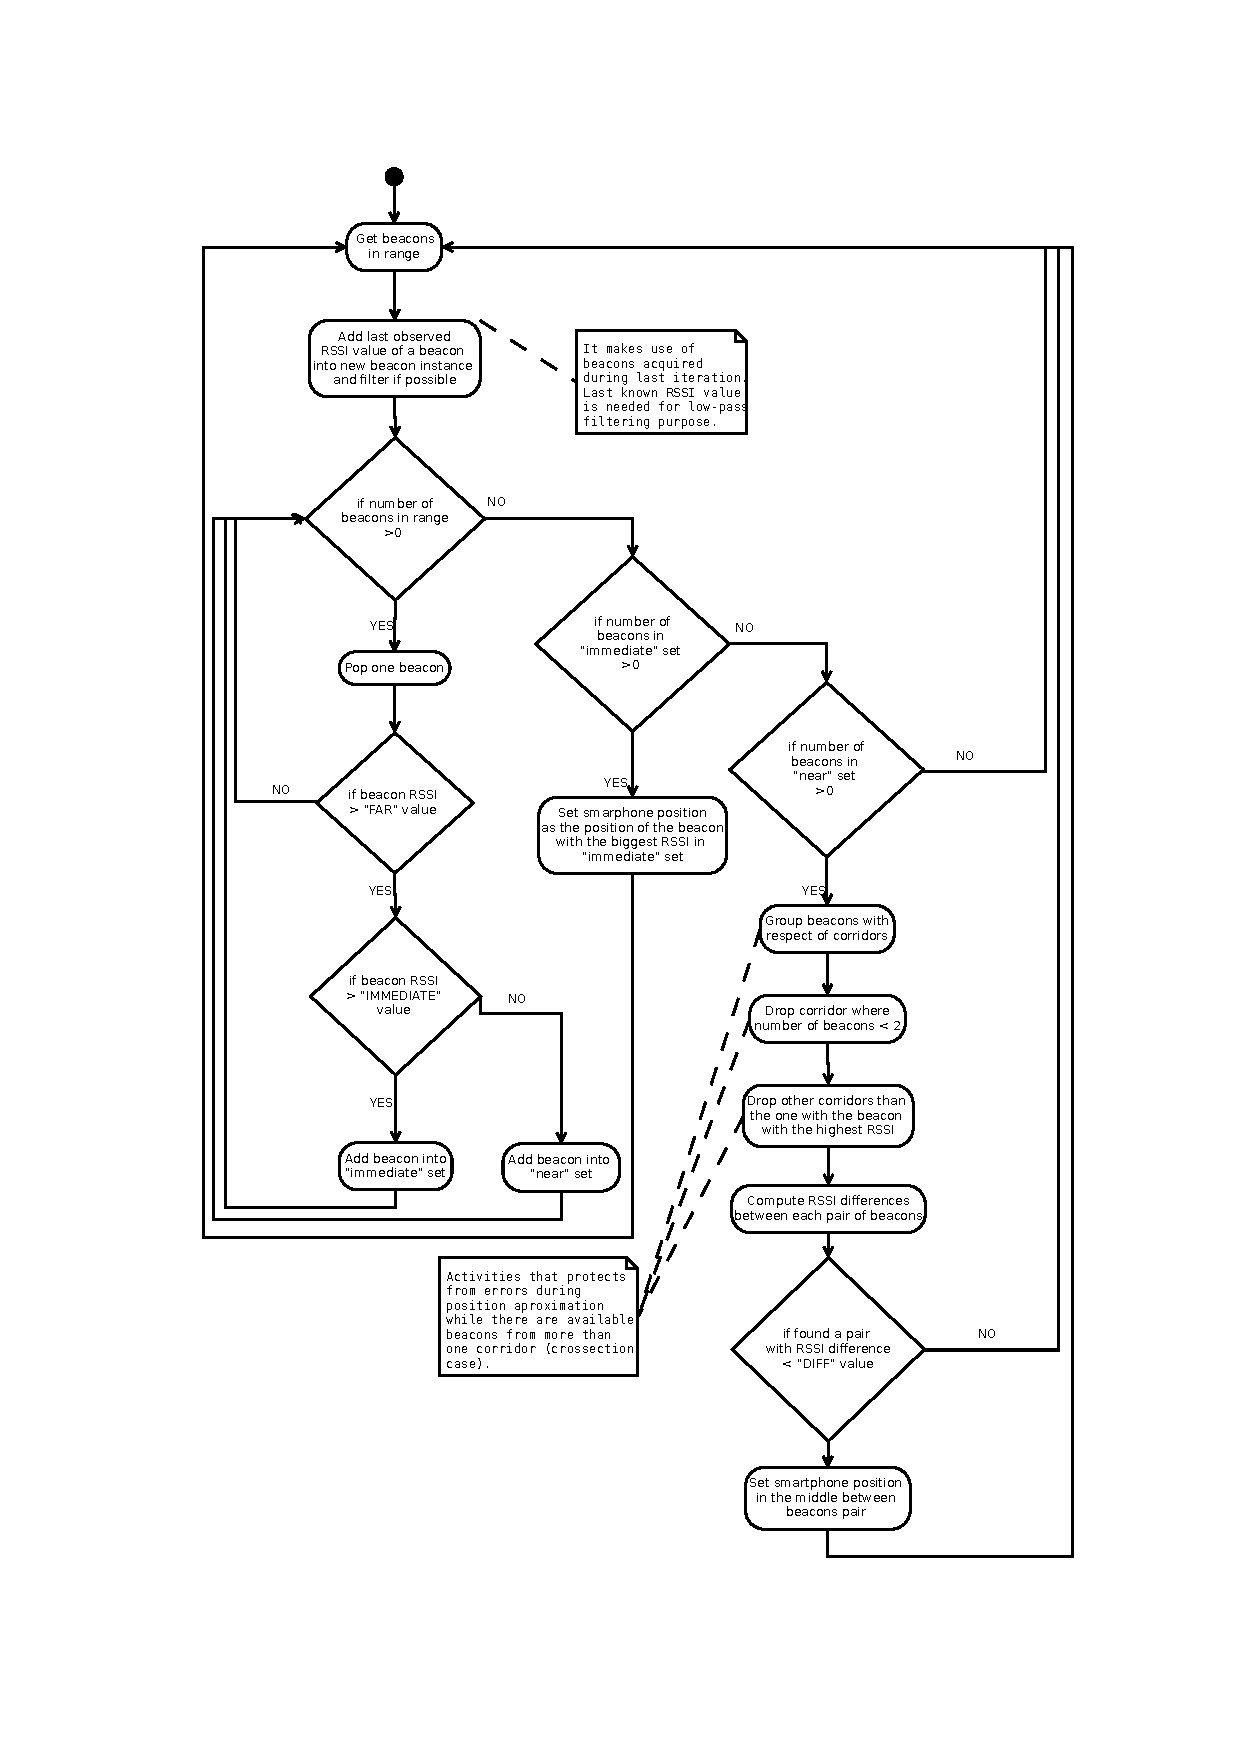
\includegraphics[width=0.9\textwidth, trim={2cm 2cm 2cm 2cm},clip]{pictures/architecture_beacons_processing.pdf}
\centering
\caption{Porposed position aligning method based on the received signal strengths from reference points.}
\label{fig:architecture_beacons_processing}
\end{figure}

Figure \ref{fig:architecture_beacons_processing} presents the concept of the received signal strength based positioning solution for smartphones. As application of the distance models on the RSS values are questionable in underground installation envioronment, the proposed solution relies on predifined values expresing the distance class rather than on approximated distances based on exact received signal strenth analysis. Values used for the positioning system were computed from results obtained during the underground tests. Proposed algorithm for position approximation use three predefined values:
\begin{enumerate}
	\item FAR threshold - RSS value that describes minimum RSS that can be taken into consideration during approximate position evalutaion. Beacon that send signals with lower RSS than defined by "FAR" is categorised as "far beacon" and signal is treated as a noise,
	\item IMMEDIATE threshold - RSS value that descibes minimum RSS that comes from the beacon located "immediate" to the smarpthone. Signals with bigger RSS value indicates that beacon that emmited those signals is an "immediate beacon". Signals with smaller RSS, but larger that defined by FAR threshold, indicates that beacon that emmited those signals is a "near beacon",
	\item DIFF value - maximum accepted difference between obtained RSS values from signals sent by "near beacons" that allows to approximate the smartphone positinon in the middle of those "near beacons".
\end{enumerate}

In simple case, where smartphone is away from corridor crossections, position finding algorithm is aware of two positioning senarios: smartphone is close ("immediate") to the beacon and smartphone is in between two near beacons. In order to determine current scenario, algorithm computes RSS of all signals received and categories them with respect of thier values into two sets: "immediate" and "near". If there were found "immediate" classified beacons then algorithm set current smartphone position to the position of the "immedieate" beacon with the biggest RSS value. In case where there are no "immediate" beacons but there were found at least two "near" beacons then the difference between their RSS values are evaluated. If difference is lower than DIFF value then the smartphone position is considered as in the middle of related beacons.

Is is possible that smartphone device is near the corridor crossection. In that case it is smartphone receive signals from beacons located in two or even more corridors (like in case of crossections in room-and-pillar production block -- see figure \ref{fig:room_and_pillar_scheme}). In such situation there is need to adjust algorithm to make use from informations from beacons labeled with different corridors names and meters related to the given corridors. Proposed solution is about finding the immediate beacon first. If there is no such beacon then RSS values from all "near" beacons are evaluated in order to check if there is possibility to estimate smartphone position as position in the middle of two nearby beacons. For that purpose beacons are grouped into sets that represents corridors they belong to. Sets with only one beacon are removed. Within all remaining sets algorithm look for a pair of similiar RSS values (difference must be smaller than DIFF threshold). If such pair was found then smartphone position is estimated as a position in the middle of beacons that emmits signals from pair.

% section solution_architecture (end)

\section{External solution infrastructure} % (fold)
\label{sec:external_solution_infrastructure}

Reference points infrastructure is a vital part of the proposed positioning system. In order to provide realiable reference information there is need ensure that installation is easily maintable, infrastructure parts are in good condition and were placed in defined way with accordance to the position, orientation and mounting recommendations. For this purpose installation step was defined as it is shown on figure \ref{fig:infrastructure_installation_proc}. Prior to the works on site it is suggested to plan where beacons will be placed in the installation. Outcome of this plan should be a list of beacons names and the positions expressed in pairs of corridor name and a meter counted from the beggining of the corridor. Also a map with marked places where beacons will be mounted would be a good addon that will help the installation engineer with his works. Then each beacon should be labeled in accordance to the plan and configured with the name from label and recommeded transmitting power. Such preparation will shorten installation time and will avoid potential problems with missconfiguration.

\begin{figure}[!htbp]
 % trim={<left> <lower> <right> <upper>}
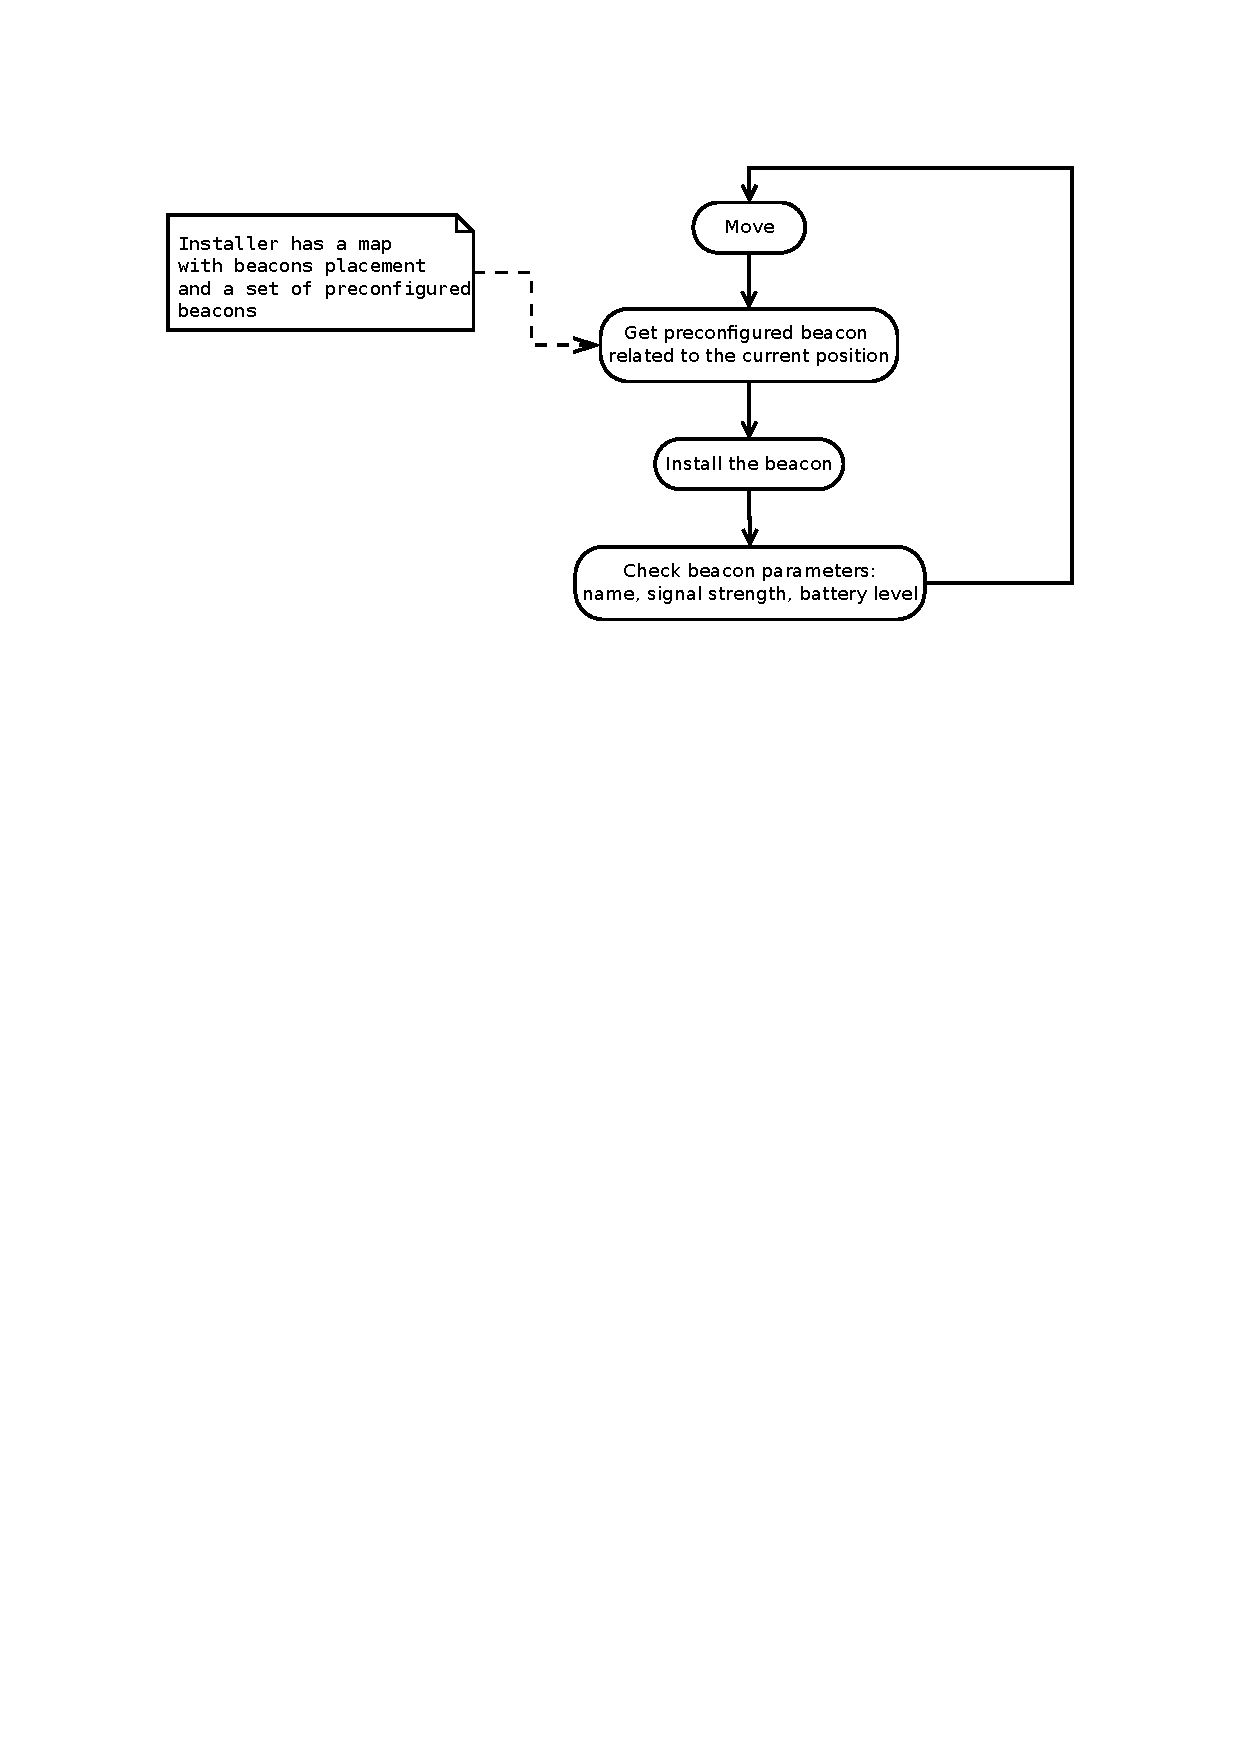
\includegraphics[width=\textwidth, trim={0 18cm 0 0},clip]{pictures/infrastructure_installation_proc.pdf}
\centering
\caption{Infrastructure installation procedure.}
\label{fig:infrastructure_installation_proc}
\end{figure}

There is need to mention in this secion
\begin{itemize}
	\item Beacons choisen as the hardware equipment.
	\item Constraints assumed - power settings, batteries sizes (capacities), distances, placement, etc
	\item Draw schematic way of infrastructure placement
	\item Mention someting about installation and maintenance procedure
	\item How beacons will be recognisable (names). What other parameters will they contain
\end{itemize}
% section external_solution_infrastructure (end)

\section{Data processing and analysis} % (fold)
\label{sec:data_processing}

Proposed positioning system depends on inputs from the smartphone's wireless receiver. Raw data cannot be used directly by the positioning algorithm because of different nature of those signals and presence of high dirfts and noise levels that affects wireless transmission. In order to make signal useful there is need to apply filtering that will normalize the outcome of particular information source and possibly improve position estimation.

There were investiaged four filtering methods:
\begin{itemize}
	\item Kalman filter,
	\item Low-pass filter,
	\item RSSI smoothing approach \cite{rssi_smoothing},
	\item Median filter.
\end{itemize}

All filteres were applied to example signal strength waveform. Results are presented on figure \ref{fig:filtering_comparison}.

\begin{figure}[!htbp]
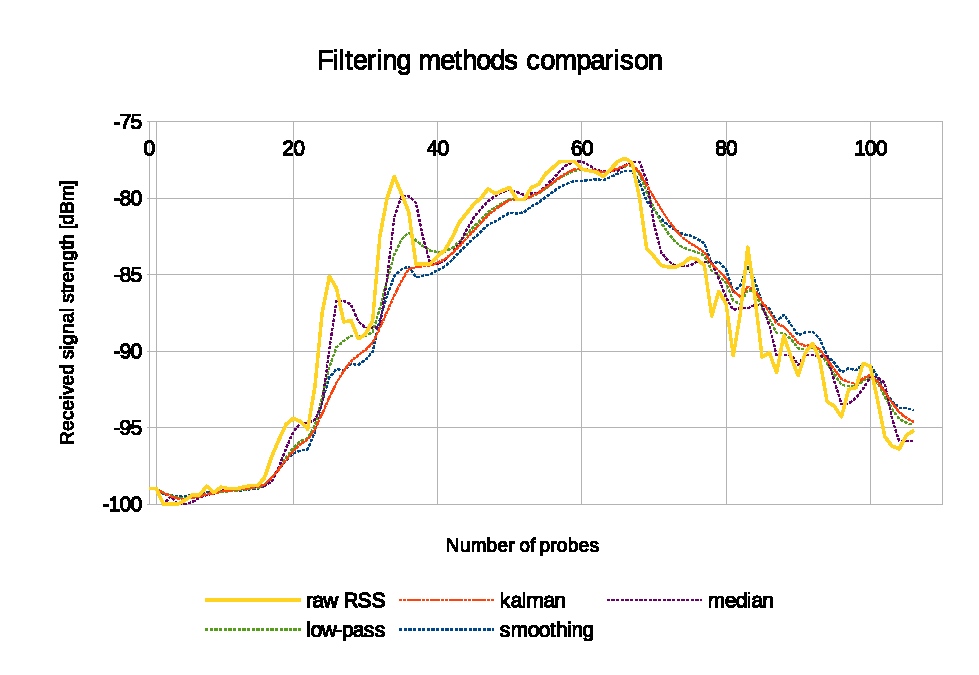
\includegraphics[width=\textwidth]{pictures/filtering_comparison}
\centering
\caption{Porposed position aligning method based on the received signal strengths from reference points.}
\label{fig:filtering_comparison}
\end{figure}

Median filter is a non-linear moving $N$--order filter. $N$ denotes number of frames within the sliding window what is directly proportional to the delay it introduces to the reslut. Aim of this filter is to obtain slow changing estimate of received signal strength curve. As the goal is to provide energy-efficient solution, the number of signal that are sent by the beacons are limited in order to safe energy. It was assumed that beacons will send signal two times per second. The value can be increased or decreased with respect of the experimentally obtained responsiveness of the positioning system and power consumption of beacons. For evaluation purposes $N=4$. As it can be observed, median filter (purple curve) doesnt fitered the RSS drop at about $30$'th probe, but filtered most of the fluctuations arround $80$'th probe. It is not accepted for a filtering function to introduce such big delay without possibility to filter fluctuations like arround $30$'th signal probe.

Smoothing RSSI approach \cite{rssi_smoothing} is a filtering method that introduces a \textit{weighted value} parameter $\alpha$ which can be any value from range $0$ -- $1$. Equation that express the method is as follows:

\begin{equation}
\label{eq:rssi_smoothing}
	RSSI_{smooth} = \alpha \cdot RSSI_n + (1 - \alpha) \cdot RSSI_{n-1}
\end{equation}

For evaluation purposes $\alpha$ parameter was set to $0.25$. Curve obtained with use of that method was distinguished on figure \ref{fig:filtering_comparison} with blue color. It was observed that this method introduces a delay of arround $4$ frames after the actual signal. Another observation is that the estimation slower than median filter reacts on the increasing and decreasing slopes of original signal: when the original curve goes up then estimate values are always bellow the original slope, when the curve goes down then estimate values are always above the original slope.

Low-pass filter is commonly used for removing short term variance from the signal. It is widely used in indoor navigation applications, mainly for inertial navigation and sensoric data analysis \cite{indoor_positioning_for_ar}\cite{indoor_navi_for_android2}\cite{report_indoor_navi_for_smartphones}\cite{thesis_ins_algorithms_for_android}\cite{indoor_positioning_for_ar_PhD_GOOD}. This approach uses cut-off parameter $\alpha$, similiar to one from smoothing approach.

\begin{equation}
\label{eq:low-pass_filter}
	RSSI_{low-pass} = RSSI_{n} + \alpha \cdot (RSSI_{n-1} - RSSI_{n})
\end{equation}

For evaluation purposes $\alpha$ parameter was set to $0.25$. Low-pass filter introduce smaller delay than in case of smooth and median filters, about $2$--$3$ frames. It filtered the signal drop arround $30$'th signal probe and fluctuations arround $80$'th probe. On figure \ref{fig:filtering_low-pass} there are presented filtering results with use of different custom extensions to the filtering method.

\begin{figure}[!htbp]
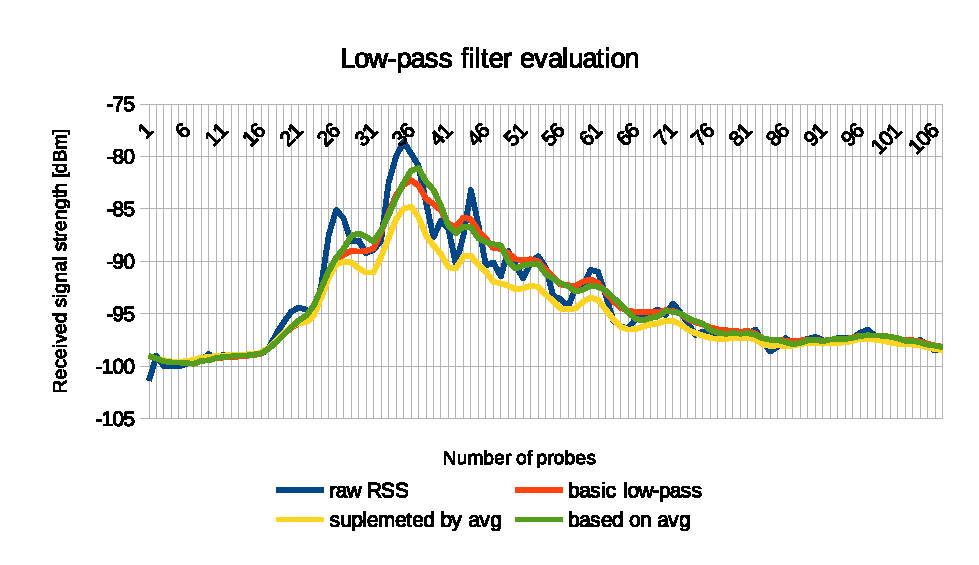
\includegraphics[width=\textwidth]{pictures/filtering_low-pass}
\centering
\caption{Porposed position aligning method based on the received signal strengths from reference points.}
\label{fig:filtering_low-pass}
\end{figure}

Custom variations of low-pass filter are a try of adjusting the responsiveness of the filter and it's fluctuation filtering capabilities. On figure are presented following concepts: low-pass filter based on average and low-pass filter suplemented by average. Following equations describe each of them:

\begin{equation}
\label{eq:low-pass_filter_avg_based}
	RSSI_{low-pass_as} = AVG(RSSI_{n-3}:RSSI_{n}) + \alpha \cdot (RSSI_{n-1} - RSSI_{n})
\end{equation}

\begin{equation}
\label{eq:low-pass_filter_avg_supplemented}
	RSSI_{low-pass_ab} = RSSI_{n} + \alpha \cdot (RSSI_{n-1} - AVG(RSSI_{n-3}:RSSI_{n}))
\end{equation}

AVG is an average function over window that consists of $4$ frames.

Kalman filter is an extended filter that allows for sensor fusioning by defining observation and transition models, and controls. It is widely used for sensor fusion of inertial navigation purposes\cite{inertial_navi_velocity_model}, also for smartphones \cite{inertial_navi_bike}\cite{indoor_navi_for_android}\cite{thesis_smartphone_inertial_plus_rfid} and Bluetooth technology \cite{beacon_rssi_analysis}\cite{discover_beacons_and_position}\cite{article_indoor_ble_rssi_filtering}\cite{article_inertial_active_beacons_calculus_kalman}. Simplified Kalman filter assumes that beacons (signal transmitters) are not moving and do not change it's state thourgh consequitive RSS readings (transition model is expressed by identity matrices). Such simplified version of a filter can be descibed as follows:

\begin{equation}
\label{eq:kalman_simplified}
\begin{aligned}
& C_n = P_{n-1} + PN	\\
& M_n = |RSSI_n-RSSIk_{n-1}|^P \cdot N + E	\\
& G_n = \frac{C_n}{C_n \cdot M_n}	\\
& P_n = \max\{PN, C_n - (G_n \cdot C_n)\}	\\
& RSSIk_n = RSSIk_{n-1} + G_n \cdot (RSSI_n -  RSSIk_{n-1})
\end{aligned}
\end{equation}

Symbols used in equation \ref{eq:kalman_simplified}:
\begin{itemize}
	\item $RSSIk_n$ -- prediction for the the $n$'th signal probe (RSS),
	\item $G_n$ -- Kalman gain for the $n$'th signal probe,
	\item $RSSI_n$ -- real measurement of $n$'th signal probe,
	\item $C_n$ -- certainity of $n$'th signal measurement,
	\item $P_n$ -- prediction certainity of $n$'th signal probe,
	\item $M_n$ -- measurement noise for $n$'th signal probe,
	\item $P$ -- measurement expotentional constraint,
	\item $N$ -- measurement noise factor constraint,
	\item $E$ -- measurement noise epsilon constraint,
	\item $PN$ -- prediction process noise constraint.
\end{itemize}


\begin{figure}[!htbp]
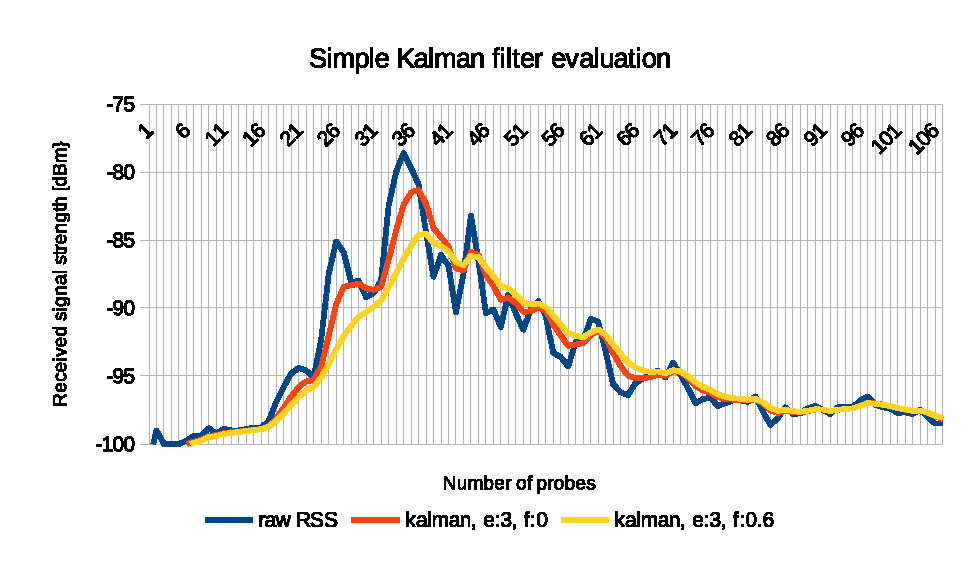
\includegraphics[width=\textwidth]{pictures/filtering_simple_kalman}
\centering
\caption{Application of Kalman filter. Red curve represent Kalman filter with $E=3$ noise constraint and $P=0$ expotentional constraint while yellow curve represent Kalman filter with $E=3$ noise constraint and $P=0.6$ expotentional constraint. }
\label{fig:filtering_simple_kalman}
\end{figure}

Figure \ref{fig:filtering_simple_kalman} presents Kalman filter applied on RSS values recorded experimenal session. With respect of chosen filter constraints it is possible to increase or decrease filter responsiveness. Increasing responsiveness cause filter faster response to changes but make it more sensitive for longer term fluctuations like in case one between $26$ and $36$ probe. Within this range red curve introduces delay of $3$ frames but does not filter the fluctuation, while yellow curve filter the fluctuation with the same delay of $3$ frames, but predicted value is about $5dBm$ lower than registered pick. Missconfigured Kalman filter overact on changes and introduces new fluctuations like it is presented on figure \ref{fig:filtering_simple_kalman_missconfigured}.

\begin{figure}[!htbp]
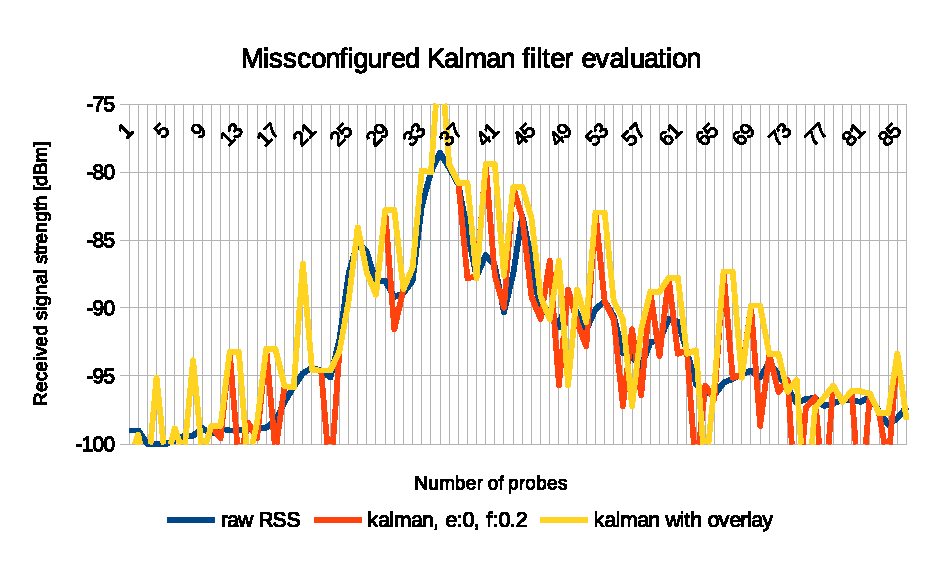
\includegraphics[width=\textwidth]{pictures/filtering_simple_kalman_missconfigured}
\centering
\caption{Application of Kalman filter. Red curve represent Kalman filter with $E=0$ noise constraint and $P=0.2$ expotentional constraint while yellow curve represent Kalman filter but with overlay }
\label{fig:filtering_simple_kalman_missconfigured}
\end{figure}


% TODO - move it to the post processing/ filtering techniques section
Values of signals strength cannot be used directly as an input for because models are sensitive on the provided signal strengths. That is why filtering techniques are needed in order to make the signal free from random changes and more robust in terms of environmental distortions. There are known other filtering approaches dedicated for RSS like Gaussian filter, distance weighted filter or propagation model training \cite{article_rssi_learning_and_filtering_for_navi} -- their applicability for underground environment will be evalueted in future works.

% section data_processing (end)

\section{Position finding algorithm implementation} % (fold)
\label{sec:simple_position_finding_algorithm_implementation}

Description of android framework, project components, problems occured, pitfails and remedies
% section simple_position_finding_algorithm_implementation (end)

\chapter{Localization system tests}

In order to check if the proposed solution is good enough to estimate the position of the mobile phone there was performed tests of chosen hardware components as well as proposed infrastructure that extends the environment and serve as the referencing system. There were performed tests of inertial navigation part of the solution by reviewing the outcome of the internal sensorics of the chosen smartphone under perspective of thier applicability to the positioning estimation algorithm. Finally there were performed tests the prototype software application that combines both environmental information from the reference points and the inertial navigation in the real environment, in underground part of Stara Kopalnia museum placed on the site of the former Coal Mine in Wałbrzych.

\section{Tests criteria and assumptions} % (fold)
\label{sec:tests_criteria_and_assumptions}

In order to test the reference system infrastructure there was need to test reference point device (Beacon transmitter) in context of interaction between this device and the receiver (Smartphone). For the hardware testing, there were following factors being specified:
\begin{itemize}
	\item receiver distance from the transmitter,
	\item smartphone orientation,
	\item smartphone model,
	\item transmitter type,
	\item transmitter power,
	\item transmitter placement,
	\item transmitter antenna direction,
	\item distance between transmitters.
\end{itemize}

Those factors were assumed that impacts the final received signal strength value.

According to \textit{Log-distance path loss model} \cite{RSSI_path_loss_prediction_model} the distance between receiver and transmitter is the major factor that impacts on the signal strength. There was need to check how distance impacts on the signal strength in the desired environment in the underground corridor.

As the Beacon operates on the 2,4 GHz fequency then it is assumed that all of the transmission path elements can impact on the resultant power strength. That is why during the tests there was checked if different antenna orientations of the transmitter and  receiver causes different results. In case of the transmitter antenna orientation there were tested two cases:
\begin{enumerate}
	\item vertical orientation where antenna points to the floor,
	\item horizontal orientation where antenna points to the wall (or the oposite wall in case of mounting the antenna on the wall).
\end{enumerate}

During tests there were tested omni directional antennas build into Beacon and mobile phone hardware as they are commonly used in Beacons as well as in Smartphones devices. It was also experimentally proven that in case of 2,4 GHz wireless technologies in underground envioronment directional antennas do not increase usable coverage as well as sector anntennas \cite{Thesis_CM}.

As the proposed solution have to be applicable for different models of Smartphone devices it is not acceptable to force users to held their devices in a given position with respect of the direction of the Bluetooth antennas build into them. Producents are free in terms of designing the Smartphones main boards including the antennas placement. Such informations are not published. Even having the possibility to open the device and look for the antenna it is diffcult to distinguish the antenna used for Bluetooth from the other used for example for terrestrial mobile networks. In case of Beacons, antenna placement is visible from the first sight. On figure \ref{fig:beacons_used_in_tests} antenna placements was highlighted. In case of Beacon 1 and 3 there are mounted meander monopol antennas, in case of Beacon 2 there is mounted called meander "IFA" -- \textit{Inverted-F antenna}, in case of Beacon 4 antenna is not visible on the picture.

\begin{figure}[!htbp]
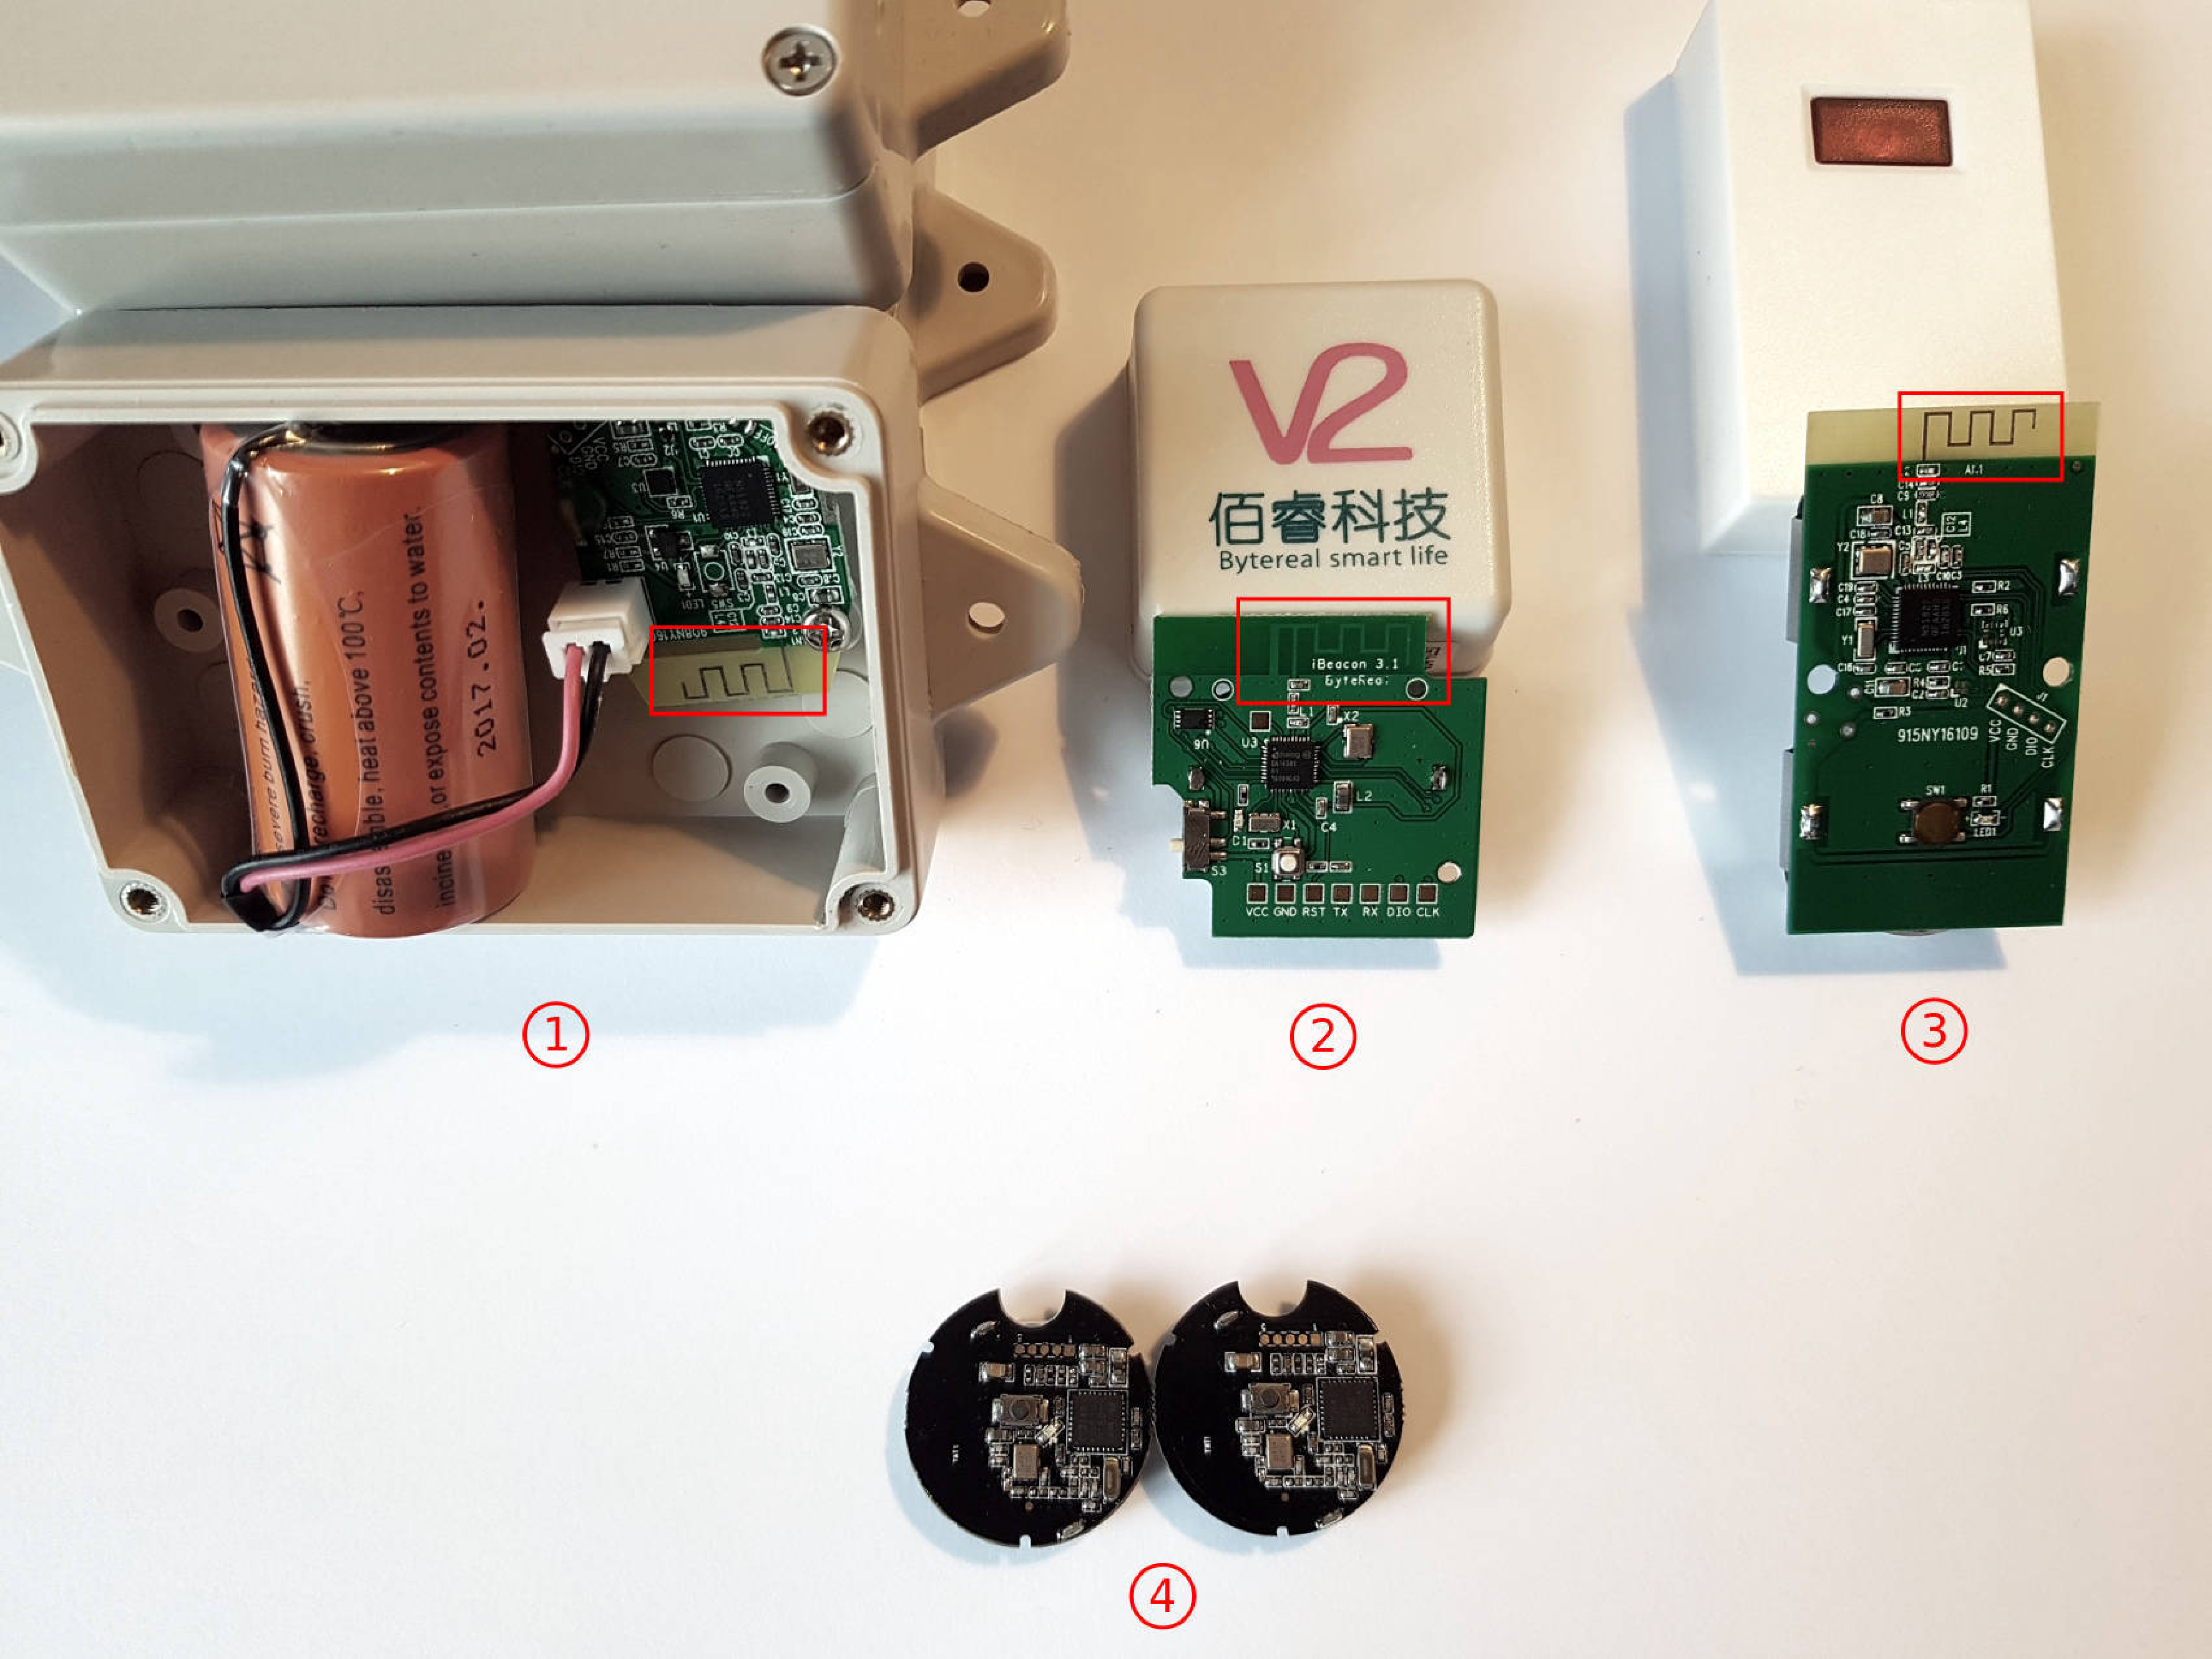
\includegraphics[width=\textwidth, keepaspectratio]{pictures/beacons_used_in_tests.pdf}
\centering
\caption{Beacons transmitters used during tests. Beacon 1 is a Wellcore procduct based on Nordic Semiconductor NRF51822 chip, Beacon 2 is a ByteReal product based on Dialog Semiconductor DA14580 chip, Beacon 3 is a Wellcore product based on Nordic NRF51822 chip, Beacon 4 is a Radioland product based on Texas Instruments TI2640 chip. On pictures there are highlighted antennas placement.}
\label{fig:beacons_used_in_tests}
\end{figure}

There are a few big microcontroller producents on the market that offers compound units having integrated computational resources, programming busses and data exchange solutions including Bluetooth Low Energy wireless module. The main three competitors are Nordic Semicondutor with NRF chips, Dialog Semicondutor with DA chips and Texas Instruments with TI and CC chips. They compete on fields of power consumtion, usability in terms of set of integrated modules, computational power and permament storage size of their products. Those integrated circuts are used by Beacon producents as the main processing units with implemented Bluetooth protocols and stack and set of profiles that allows the users to configure Beacon parameters such as name or transmitter power and get information from extra sensorincs measures build into the Beacon like temperature or battery level. Integrated circuts are the part of PCB which also contains a battery slot, power circut and antenna circut. For tests there were chosen Beacons offered by the various producents form China thus their products were easily available via the Internet and they were cheaper than from producents from Europe or U.S. like Estimote or Texas Instruments\cite{beacons_ble_evaluation}. Aim of tests with different Beacons was to check how much PCB design influences results in terms of antenna radiation, signal coverage and stability. In order to distinguish beacons during tests, each of them was labeled. There were used following beacons:
\begin{enumerate}
	\item Wellcore beacon based on Nordic Semiconductor NRF51822 chip, with a 8500 mAh, 3,6V lithium battery (cost: 7\$, labeled as $B1$),
	\item ByteReal beacon based on Dialog Semiconductor DA14580 chip, with a standard CR2477 battery (950 mAh, 3 V, cost: 8,25\$, labeled as $B2$),
	\item Wellcore beacon based on Nordic Semiconductor NRF51822 chip, with two standard CR277 batteries (1900 mAh, 3 V, cost: 10\$, labeled as $B3$),
	\item Radioland beacon based on Texas Instruments TI2640 chip, with a standard CR2032 battery (220 mAh, 3 V, cost: 6,78\$, labeled as $B4$).
\end{enumerate}

During tests there were following smartphone related factors taken into consideration: smartphone orientation and smartphone model. There was tested how differs received signal strength with when smartphone is hold horizontally (screen points to the ceiling), vertically (screen points to the user) or is kept in the pocket. There were also performed beacon ranging tests with use of two different smarphone devices: Samsung Galaxy S7 and Blackberry Z10. Samsung is equiped with Bluetooth 4.1 while Blackberry is equiped with Bluetooth 4.0. The aim of this test was to compare the result in order to check how different construction impact on the received signal strength. There was need to verify assumption about having defined constraint values on received signal that regardless the smartphone model will allow to qualify distance from signal source basing on acquired signal value.

Hardware tests were designed in a manner that each of those factors were tested separately. There were performed following test cases:

\begin{enumerate}
	\item Obtain signal attenuation curve with respect of the power of the transmitter by measuring the received signal stregth at given distances from the signal source.
	\item Signal range per given transmitter power setting and smartphone placed in the pocket. Dynamic tests performed on a distance of 5 meters.
	\item Received signal strength per given transmitter power setting and different smartphone orientation. Static test performed directly under the transmitter.
	\item Line of sight (LOS) test. Comparison of signal attenuation curve measured in a part of the corrdor where smartphone and transmitter were in line of sight and signal attenuation curve measured in a part of the corridor where corridor goes up and transmitter and smartphone are not in a line of sight.
	\item Test of line of sight impact on the signal attenuation curve where user is and is not an obstacle between transmitter and smartphone.
	\item Test how different antenna orientations of transmitter mounted on ceiling impacts on signal attenuation curve. Tested vertical and horizontal orientations.
	\item Test how different antenna orientations of transmitter mounted on wall impacts on signal attenuation curve. Tested vertical and horizontal orientations.
	\item Test how beacons from different vendors impacts on the signal attenuation curve. For this test beacons transmitting power was adjusted in order to obtain similiar signal gain on the radio path.
	\item Test how different smartphone models impact on the signal attenuation curve. Two different smatphones were used: Samsung Galaxy S7 with Bluetooth 4.1 and Blackberry Z10 with Bluetooth 4.0 module.
	\item Walk scenario case test. Dynamic test with three beacons mounted on the wall while the user with a smartphone is walking along them. Tested two distancess between beacons: 10 m and 15 m.
	\item Wall scenario case test. Dynamic test with three beacons mounted on the wall while the user with a smartphone is walking along them. Tested how smartphone kept in the pocket influence the attenuation curve.
	\item  Compare signal attenuation curve when transmitter is placed on the wall and when it is placed on the ceiling.
\end{enumerate}

\begin{itemize}
	\item Define factors that are important to state if solution is good or not
	\item Will allow to check if system fulfills requirements
	\item Test features stated in 'Localization system choise section'
\end{itemize}

% section tests_criteria_and_assumptions (end)

\section{Tests metodology} % (fold)
\label{sec:tests_metodology}

Tests were performed in part of XVIII century exchavation corridor which is available for sighseeing as a part of Stara Kopalnia museum in Walbrzych in Poland. Corridor used during tests is placed 10 m bellow the ground and it is 185,7 m long. Corridor is 3,2 m high and 3,2 m wide. Corridors goes up on it's north side so this part of the corridor was used only once during line of sight test case. There is also one "T" shaped crossection with a similiar, perpendicular corridor that is 157 m meter length.

\begin{figure}[!htbp]
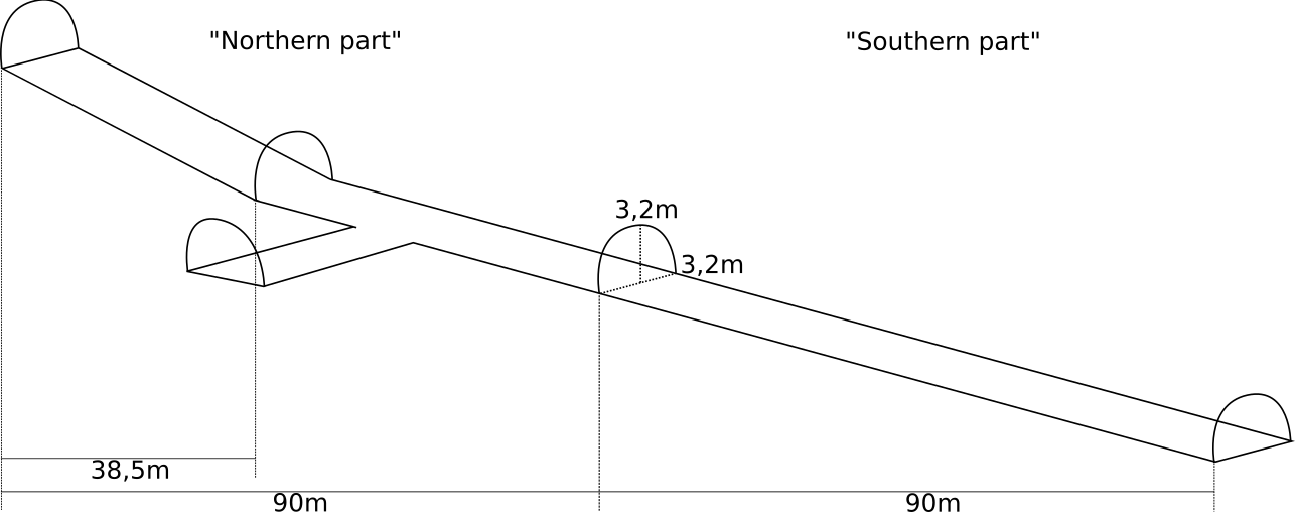
\includegraphics[width=\textwidth, keepaspectratio]{pictures/corridor.pdf}
\centering
\caption{Test place scheme.}
\label{fig:corridor}
\end{figure}

During the tests in the corridor there was $10^\circ$C  and $71 \%$ of humadity. In order to avoid diffractions from corridors endings, beacons (Bluetooth transmitters) were placed in the middle of the corridor at it's $90 m$ in case of sigle beacon test and in $\pm15 m$ from this place in case of multiple beacons test.

During the test there was used
\begin{itemize}
	\item  measuring wheel for measuring the distance between subsequent distances taken into consideration for signal attenuation charts,
	\item smartphones with application that was collecting and storing the data (Bluetooth Low Energy receivers) and
	\item prepared beacons -- Bluetooth Low Energy transmitters.
\end{itemize}

Beacons were prepared in a manner that their names were changed into B1(1), B1(2), B1(3), B2, B3 and B4 in order to distinguish them during evaluation. Beacon names were included into advertisment frame, which were then written into log files from the signal recording sessions.

\begin{figure}[!htbp]
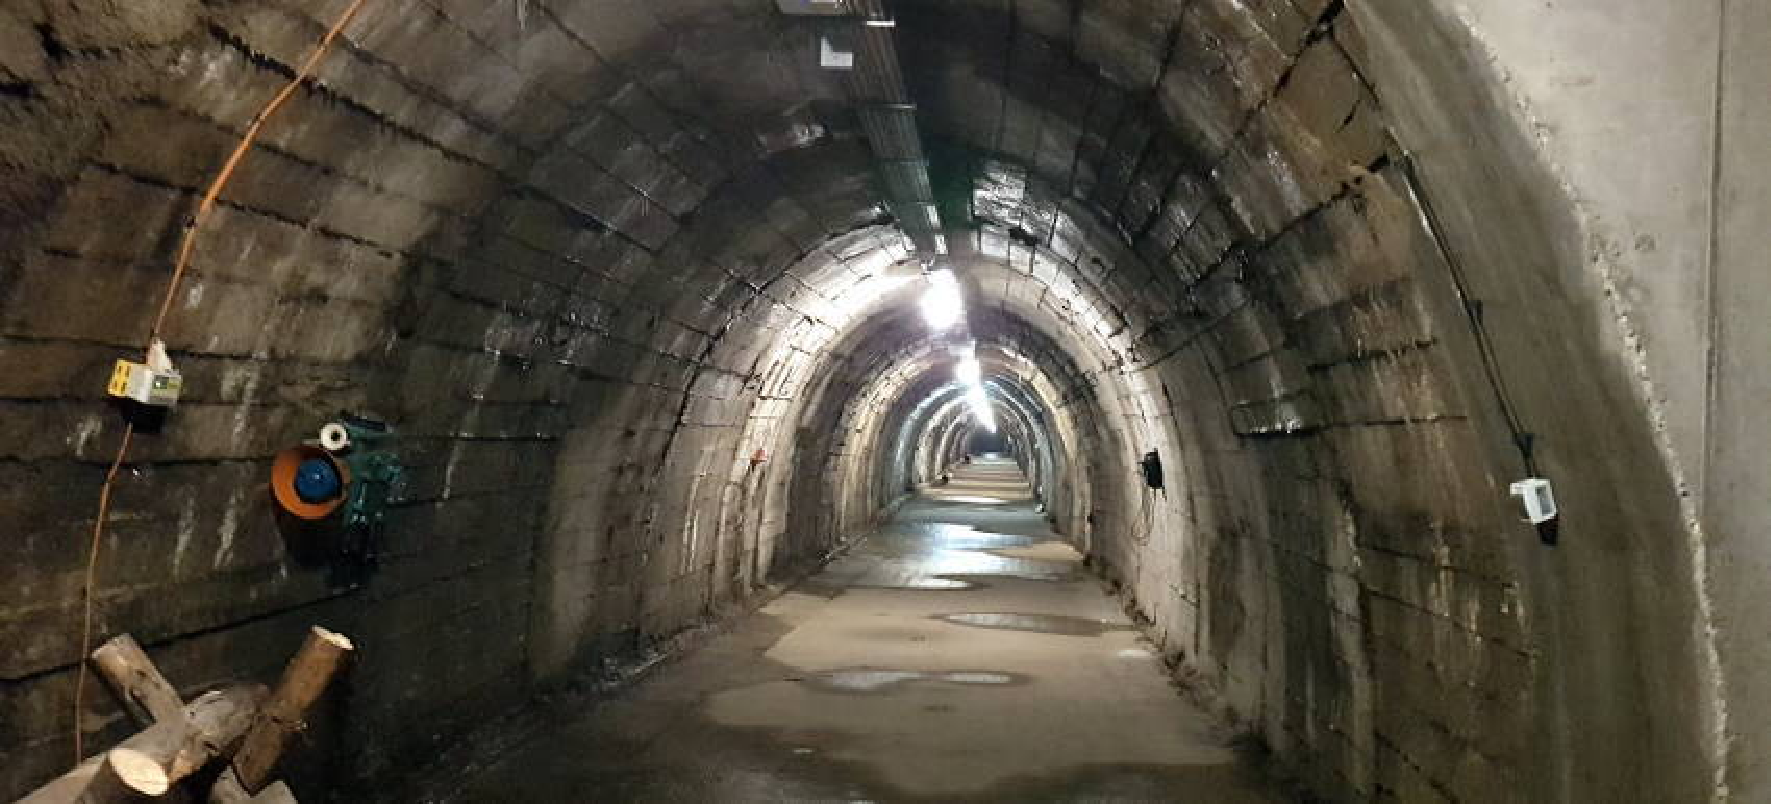
\includegraphics[width=\textwidth, keepaspectratio]{pictures/tests_corridor_general.pdf}
\centering
\caption{Side view on the test place (at the end of the corridor) from perpendicular corridor perspective.}
\label{fig:tests_corridor_genera}
\end{figure}


Scope of tests performed underground as well as the values of distinguished variables chosen for the tests, got summaried in the table \ref{tab:test_parameters}.

Symbols and terms used in the table \ref{tab:test_parameters} are following:
\begin{itemize}
	\item \textbf{Receiver} -- smartphone device that listens to the messages sended by transmitters (beacons),
	\item \textbf{Transmitter} -- bluetooth low energy device that broadcasts "advertisment" messages (beacon),
	\item \textbf{|} -- receiver orientation: smartphone is held in a vertical position, display in front of an user, user is an obstacle on line of sight, smartphone is $1m$ above the ground,
	\item \textbf{F--} --	receiver orientation: smartphone is held in a horizontal position, display points to the ceiling (content is visible to the user), user is NOT an obstacle on line of sight, smartphone is $1m$ above the ground,
	\item \textbf{B--} --	receiver orientation: smartphone is held in a horizontal position, display points to the ceiling (content is visible to the user), user is an obstacle on line of sight, smartphone is $1m$ above the ground,
	\item \textbf{P}	-- receiver orientation: smartphone is held in an user pocket, smartphone is $1m$ above the ground,
	\item \textbf{B}	-- smartphone „Blackberry Z10” device,
	\item \textbf{S}	-- smartphone „Smasung Galaxy S7” device,
	\item \textbf{TEST} -- parameter that was evaluated during the test.
\end{itemize}

\begin{table}[ht]
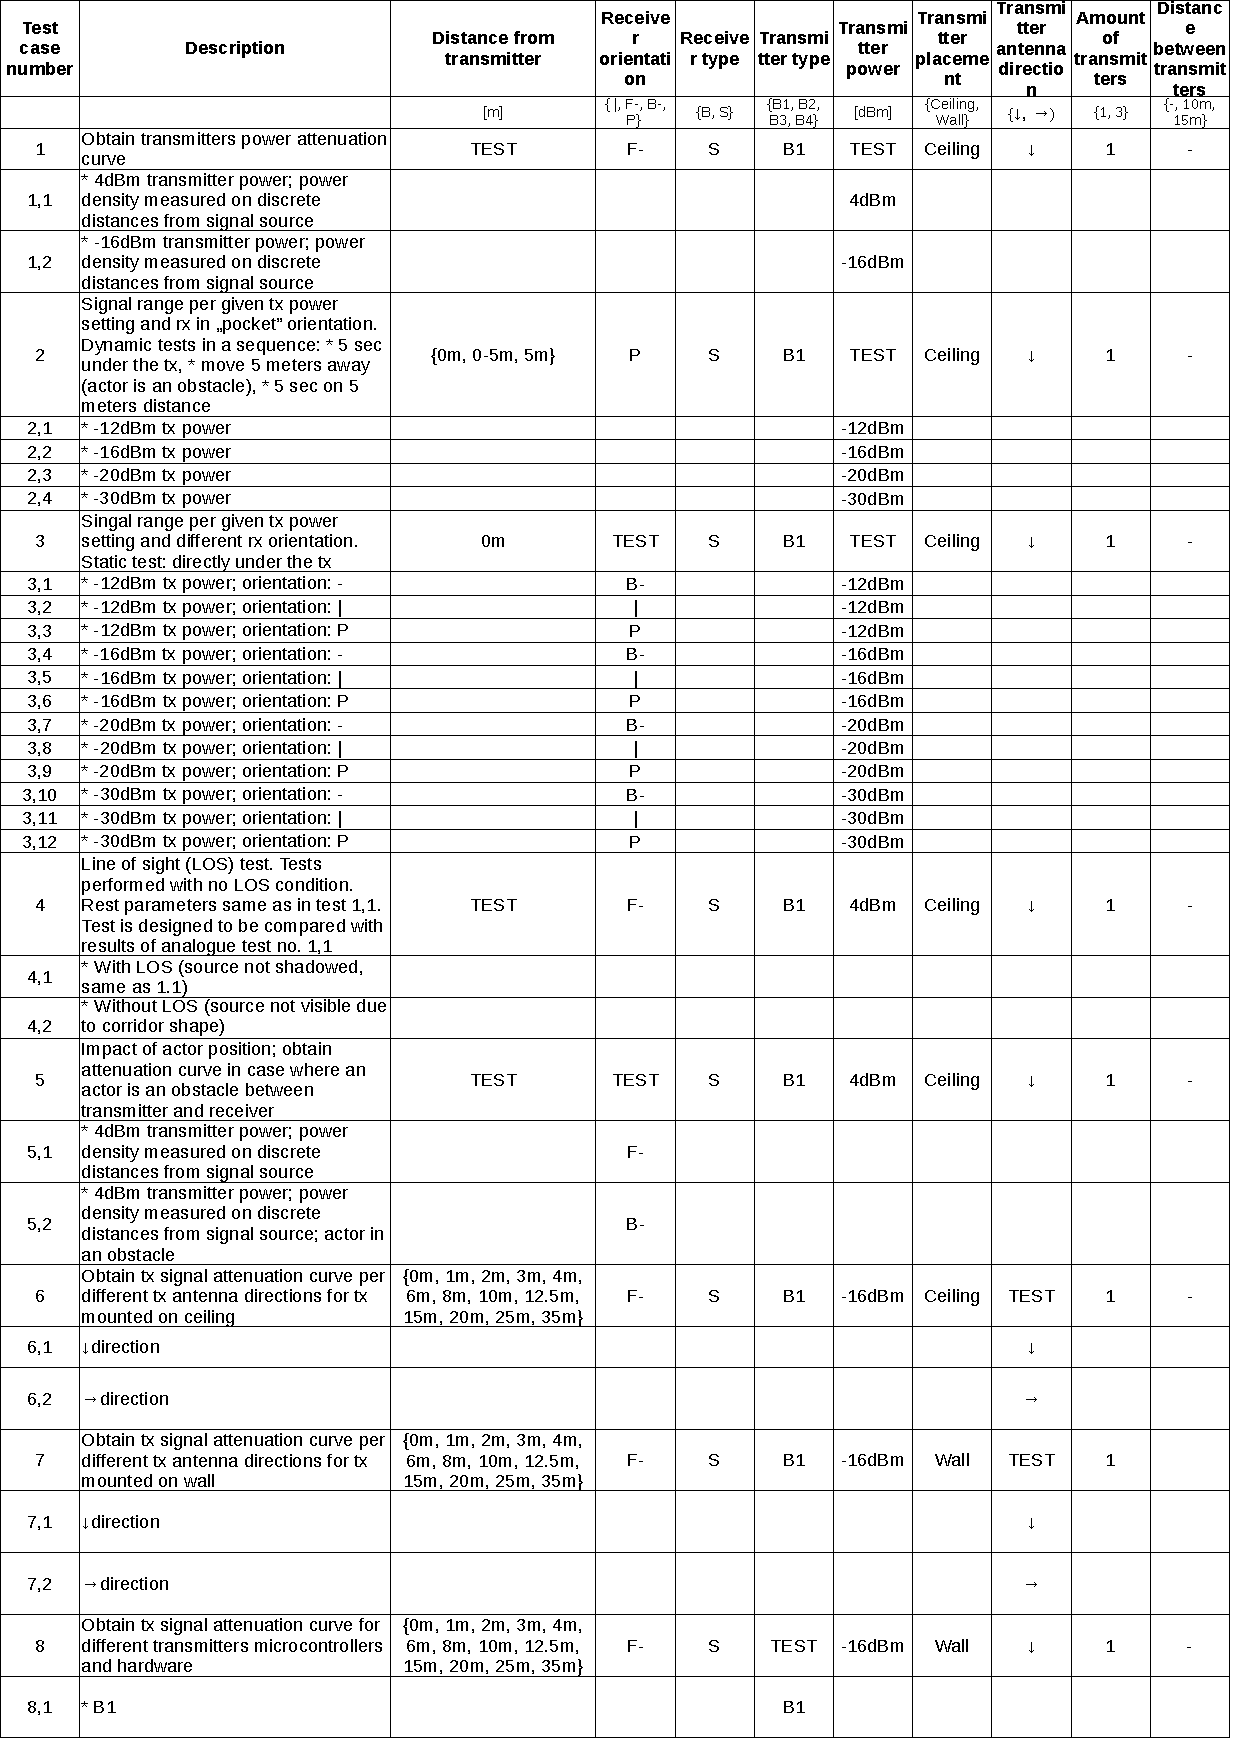
\includegraphics[width=\textwidth, keepaspectratio]{tables/test_parameters_p1.pdf}
\centering
\end{table}
\begin{table}[ht]
 % trim={<left> <lower> <right> <upper>}
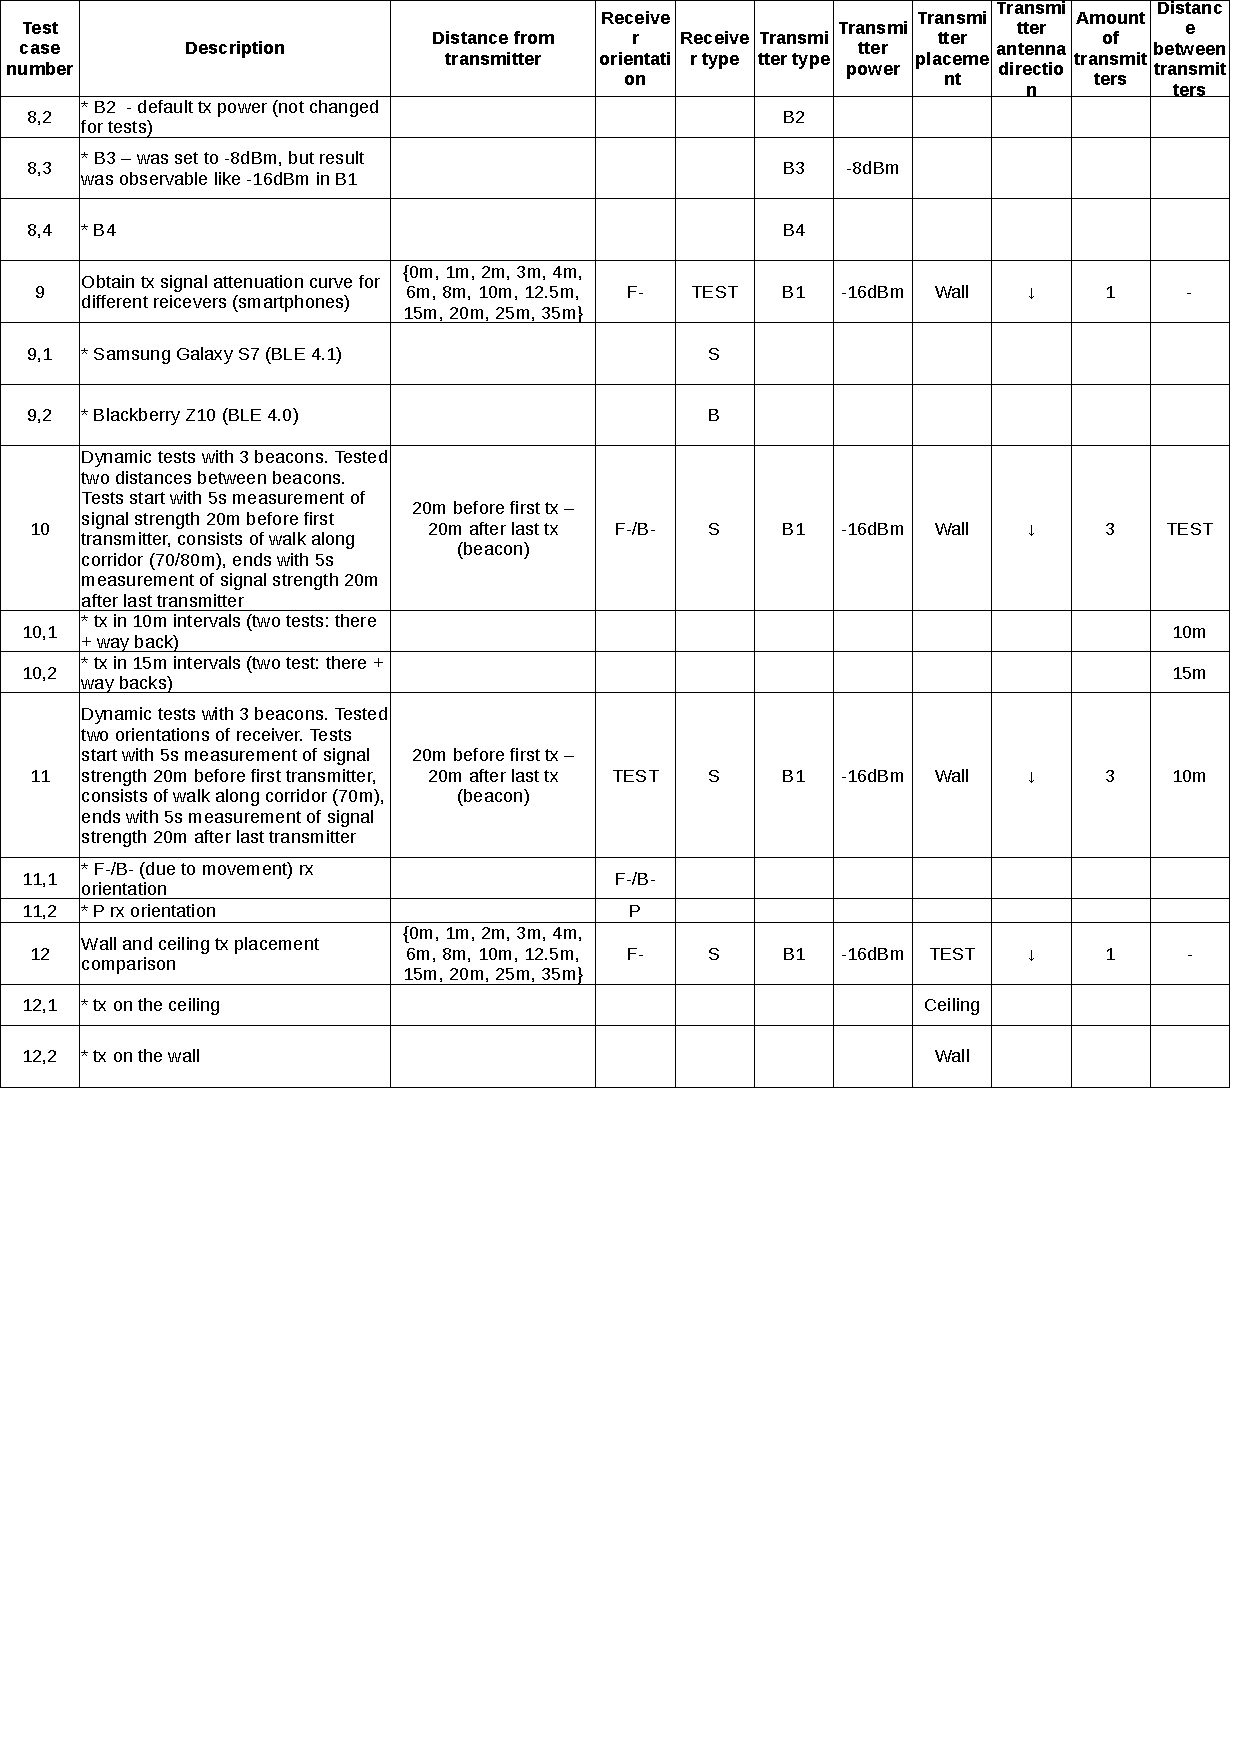
\includegraphics[width=\textwidth, trim={0 11cm 0 0},clip]{tables/test_parameters_p2.pdf}
\centering
\caption{List of test cases and related parameters.}
\label{tab:test_parameters}
\end{table}


\FloatBarrier
% section tests_metodology (end)

\section{Tests of wireless reference points in underground environment} % (fold)
\label{sec:tests_of_system_and_basic_algorithm}

The first series of tests were about observation how different factors influence the received signal strength. Factors taken into consideration, beacon and smartphone devices used during tests are listed in section \ref{sec:tests_criteria_and_assumptions}.

\subsection{Signal stability analysis} % (fold)
\label{sub:signal_stability_analysis}

As a test base there was taken a several probes of received signal strengths at different distances from the signal source. As it is shown on the figure \ref{fig:tests_case1_fluctuations_over_time}, signal strenghts are not stable in time. The general rule of \textit{log-distance path loss model}\ref{eq:log-distance-model} where the short distance between transmitter and receiver causes biger signal strengths are observed, but there are strong fluctuations in time. Model was dicussed in section \ref{sec:positioning_with_beacons_and_bluetooth_technology}.

\begin{figure}[!htbp]
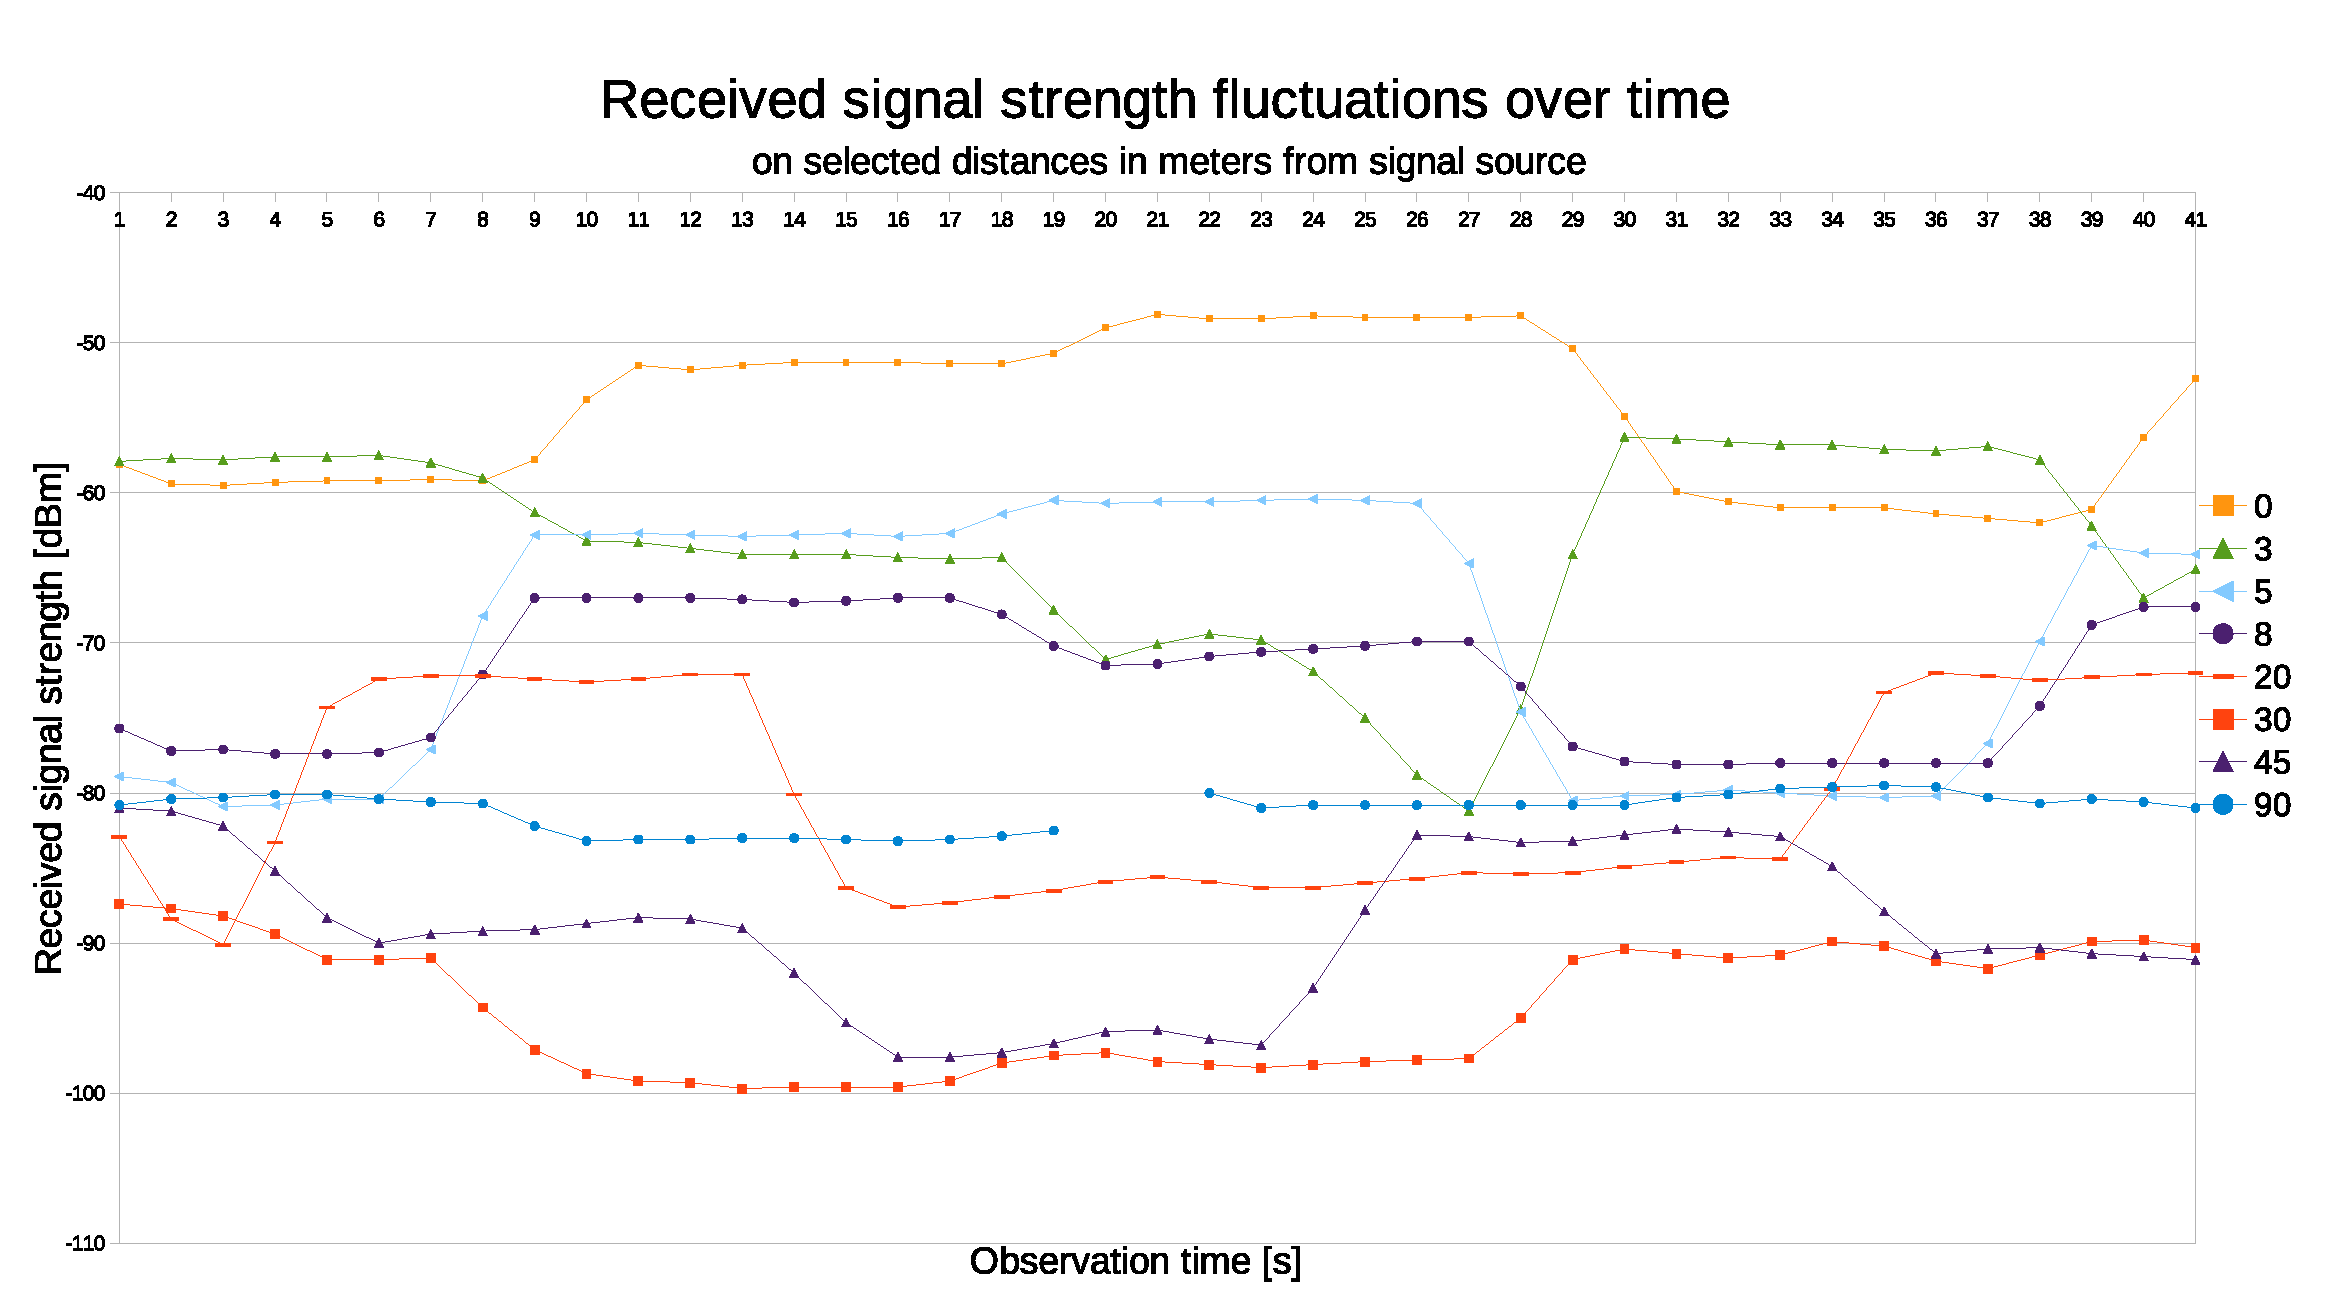
\includegraphics[width=\textwidth, keepaspectratio]{pictures/tests_case1_fluctuations_over_time}
\centering
\caption{Received signal strengths measured each second at different distances between signal source and smarphone. Each line represents received signal strength obtained at given distance.}
\label{fig:tests_case1_fluctuations_over_time}
\end{figure}

Basing on results from this test there was made obervation about the relation between the distance and the scale of fluctuation affecting the signal strengths. The biggest fluctuations are present between $0$ and $10$ meters from the signal source. On the distance of $70$ meters and more signal strengths got flatten thus also a standard deviation is low. This relation is depicted on the figure \ref{fig:tests_case1_fluctuations_over_time_std_dev}.

\begin{figure}[!htbp]
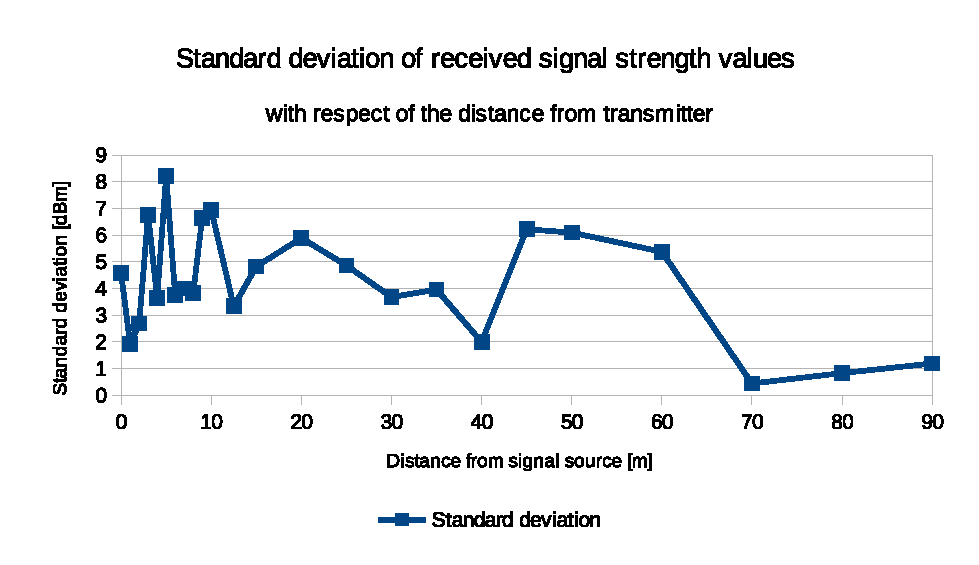
\includegraphics[width=\textwidth, keepaspectratio]{pictures/tests_case1_fluctuations_over_time_std_dev}
\centering
\caption{Standard deviation taken from received signal strengths measured each second at different distances between signal source and smarphone.}
\label{fig:tests_case1_fluctuations_over_time_std_dev}
\end{figure}

\textit{Log-distance path loss model} assumes only one input (received signal strength) what is directly a basis for distance estimation. As the model is based on logarithm (see equation \ref{eq:log-distance-model}) then fluctuactions around reference value have smaller impact on the obtained distance aproximation than the fluctuations arround the values that are away from the reference value. In order to verify how model fits into the measures then distance aproximations based on that model was computed on average values of the received signal strengths measured at given distances. There was more than 25 probes of the signal strengths taken to the average. Figure \ref{fig:tests_case1_distance_model_90m} depicts results of a aproximating the distance from beacon placed on the ceiling with the highest possible signal strength of $4dBm$ on a range of $90 m$. X-axis described the actual distance, y-axis describes approximated distance -- output of a model. Estimations in longer distances were not accurate -- they error was about $\pm 30m$ on a $20$ meters distance and more.

\begin{figure}[!htbp]
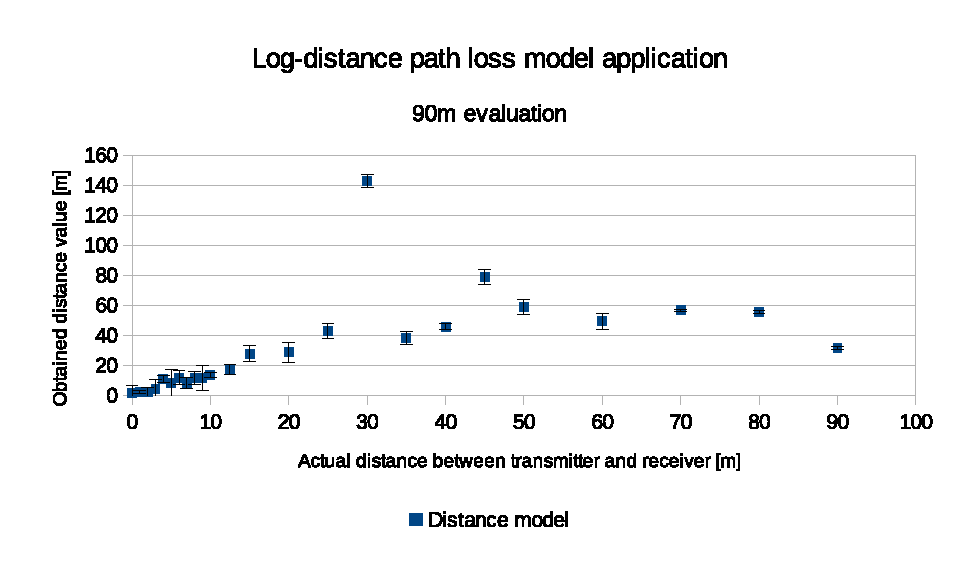
\includegraphics[width=\textwidth, keepaspectratio]{pictures/tests_case1_distance_model_90m}
\centering
\caption{Application of \textit{log-distance path loss model} on received signal strengths measured at discrete distances from signal source at range of $90m$.}
\label{fig:tests_case1_distance_model_90m}
\end{figure}


Figure \ref{fig:tests_case1_distance_model_20m} focuses on range in between $0$ and $20$ meters from signal source. In this range aproximation error was about $\pm 1.5$ meters. Such result leads to the assumtion that on distances lower than $20m$ from the signal source, proposed model can provide approximation which fits to the required accuracy stated for the positioning system.

\begin{figure}[!htbp]
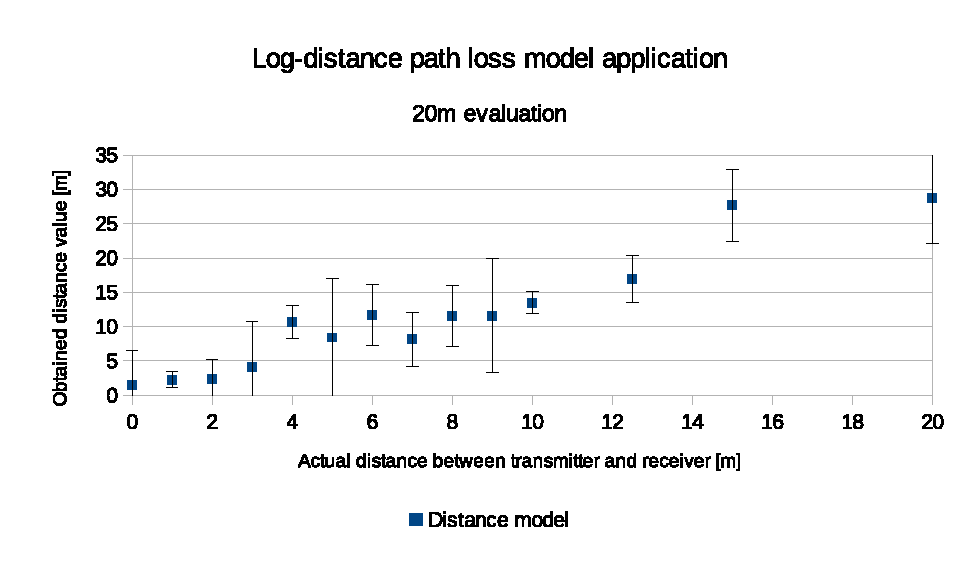
\includegraphics[width=\textwidth, keepaspectratio]{pictures/tests_case1_distance_model_20m}
\centering
\caption{Application of \textit{log-distance path loss model} on received signal strengths measured at discrete distances from signal source at range of $20m$.}
\label{fig:tests_case1_distance_model_20m}
\end{figure}

% subsection signal_stability_analysis (end)
\FloatBarrier

\subsection{Robustness of received signal strenght measures} % (fold)
\label{sub:robustness_of_received_signal_strenght_measures}


One of the objectives stated for tests was to check how placement, orientation and different models of the devices impacts the received signal strength values. List of variables taken into consideration with explanation were written in section \ref{sec:tests_criteria_and_assumptions}. Pictures \ref{fig:tests_beacon_celing_horizontal} and \ref{fig:tests_beacon_celing_vertical} presents how beacon was mounted on a ceiling with it's different orientations related to the antenna direction.

\begin{figure}[!htbp]
\begin{minipage}{0.49\linewidth}
 % trim={<left> <lower> <right> <upper>}
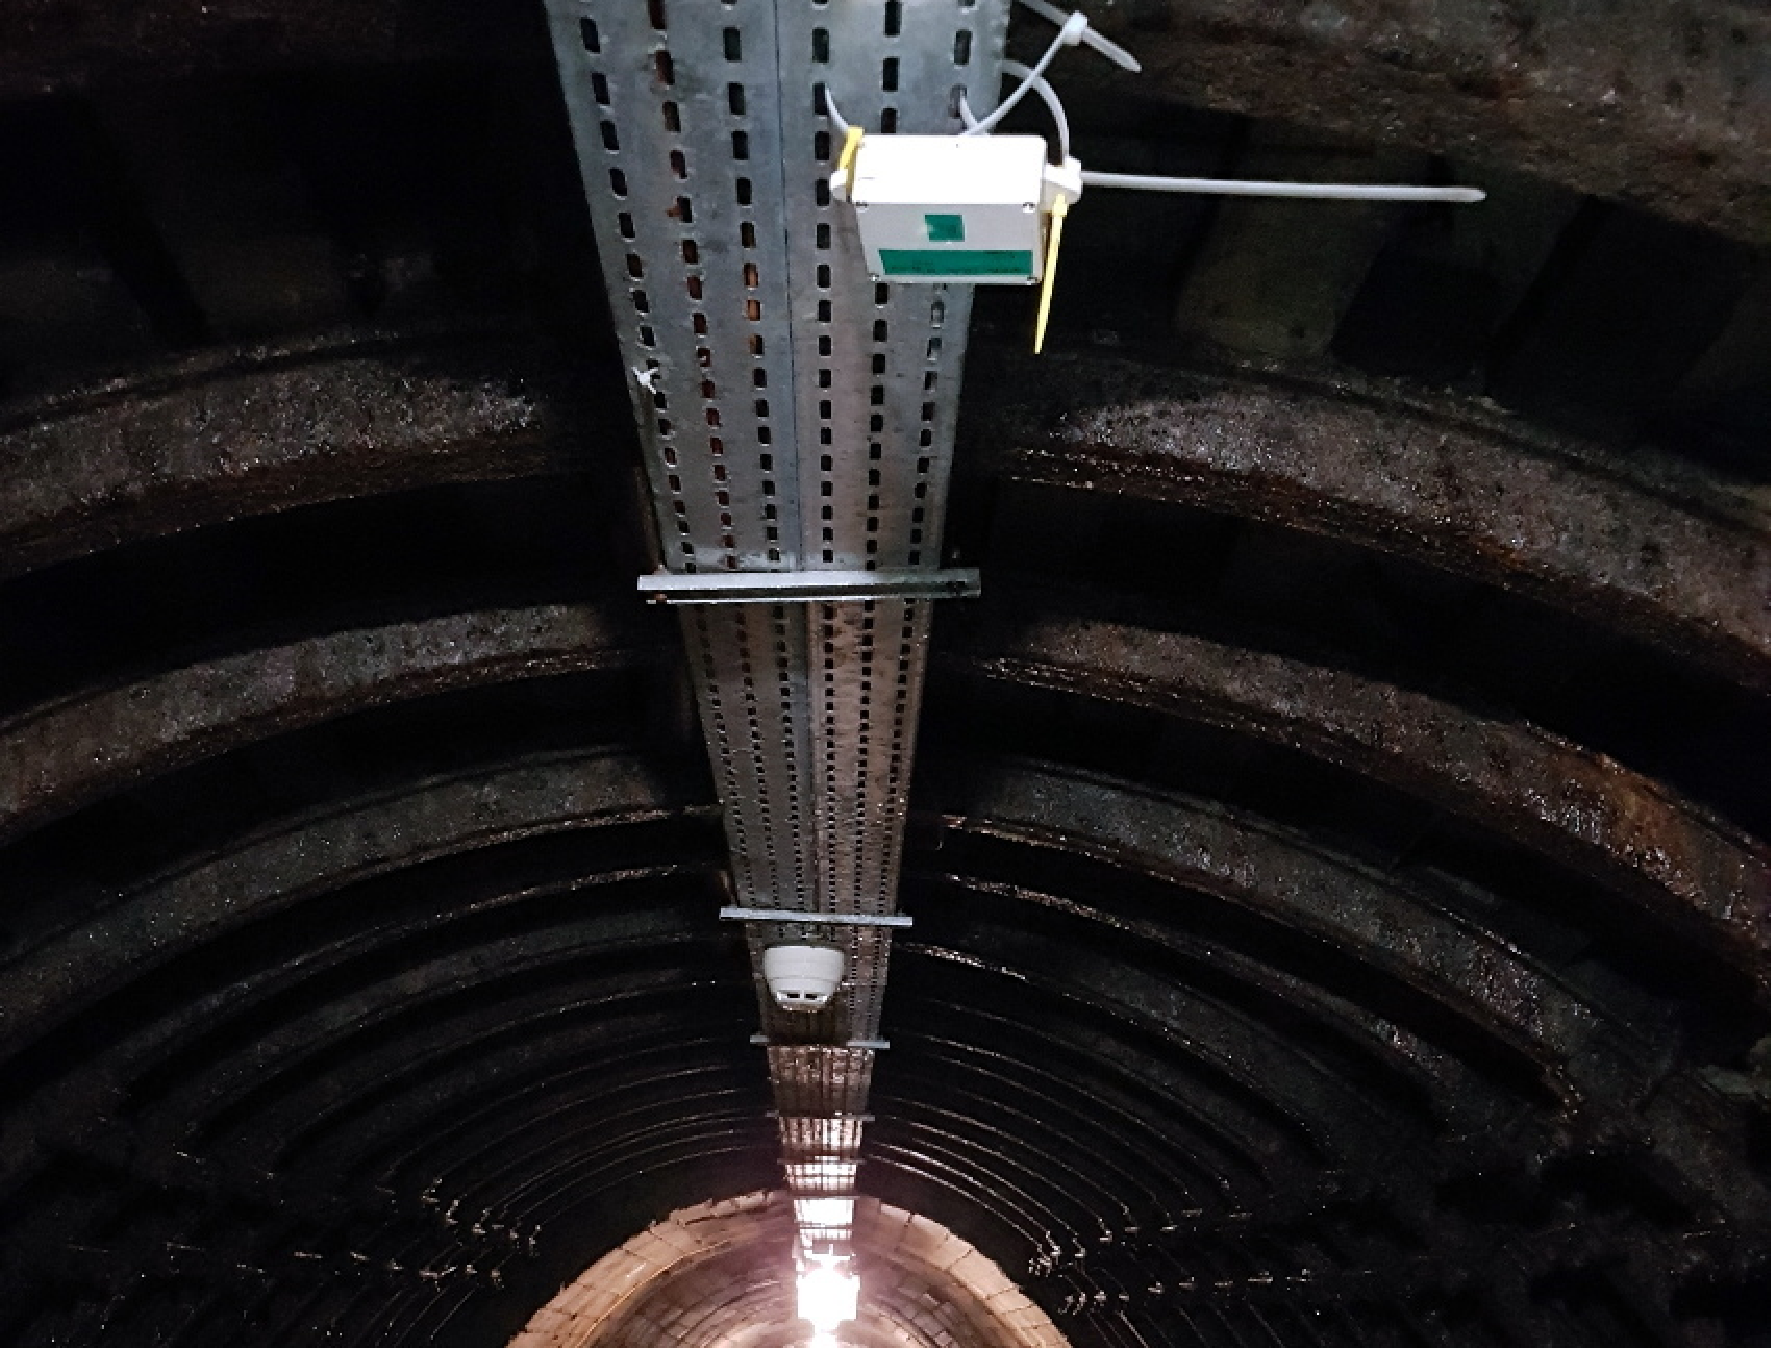
\includegraphics[width=\textwidth, trim={3cm 0 3cm 0},clip]{pictures/tests_beacon_celing_horizontal.pdf}
\caption{Beacon 1 mounterd on a ceiling with horizontal antenna direction.}
\label{fig:tests_beacon_celing_horizontal}
\end{minipage}\hfill%
\begin{minipage}{0.49\linewidth}
 % trim={<left> <lower> <right> <upper>}
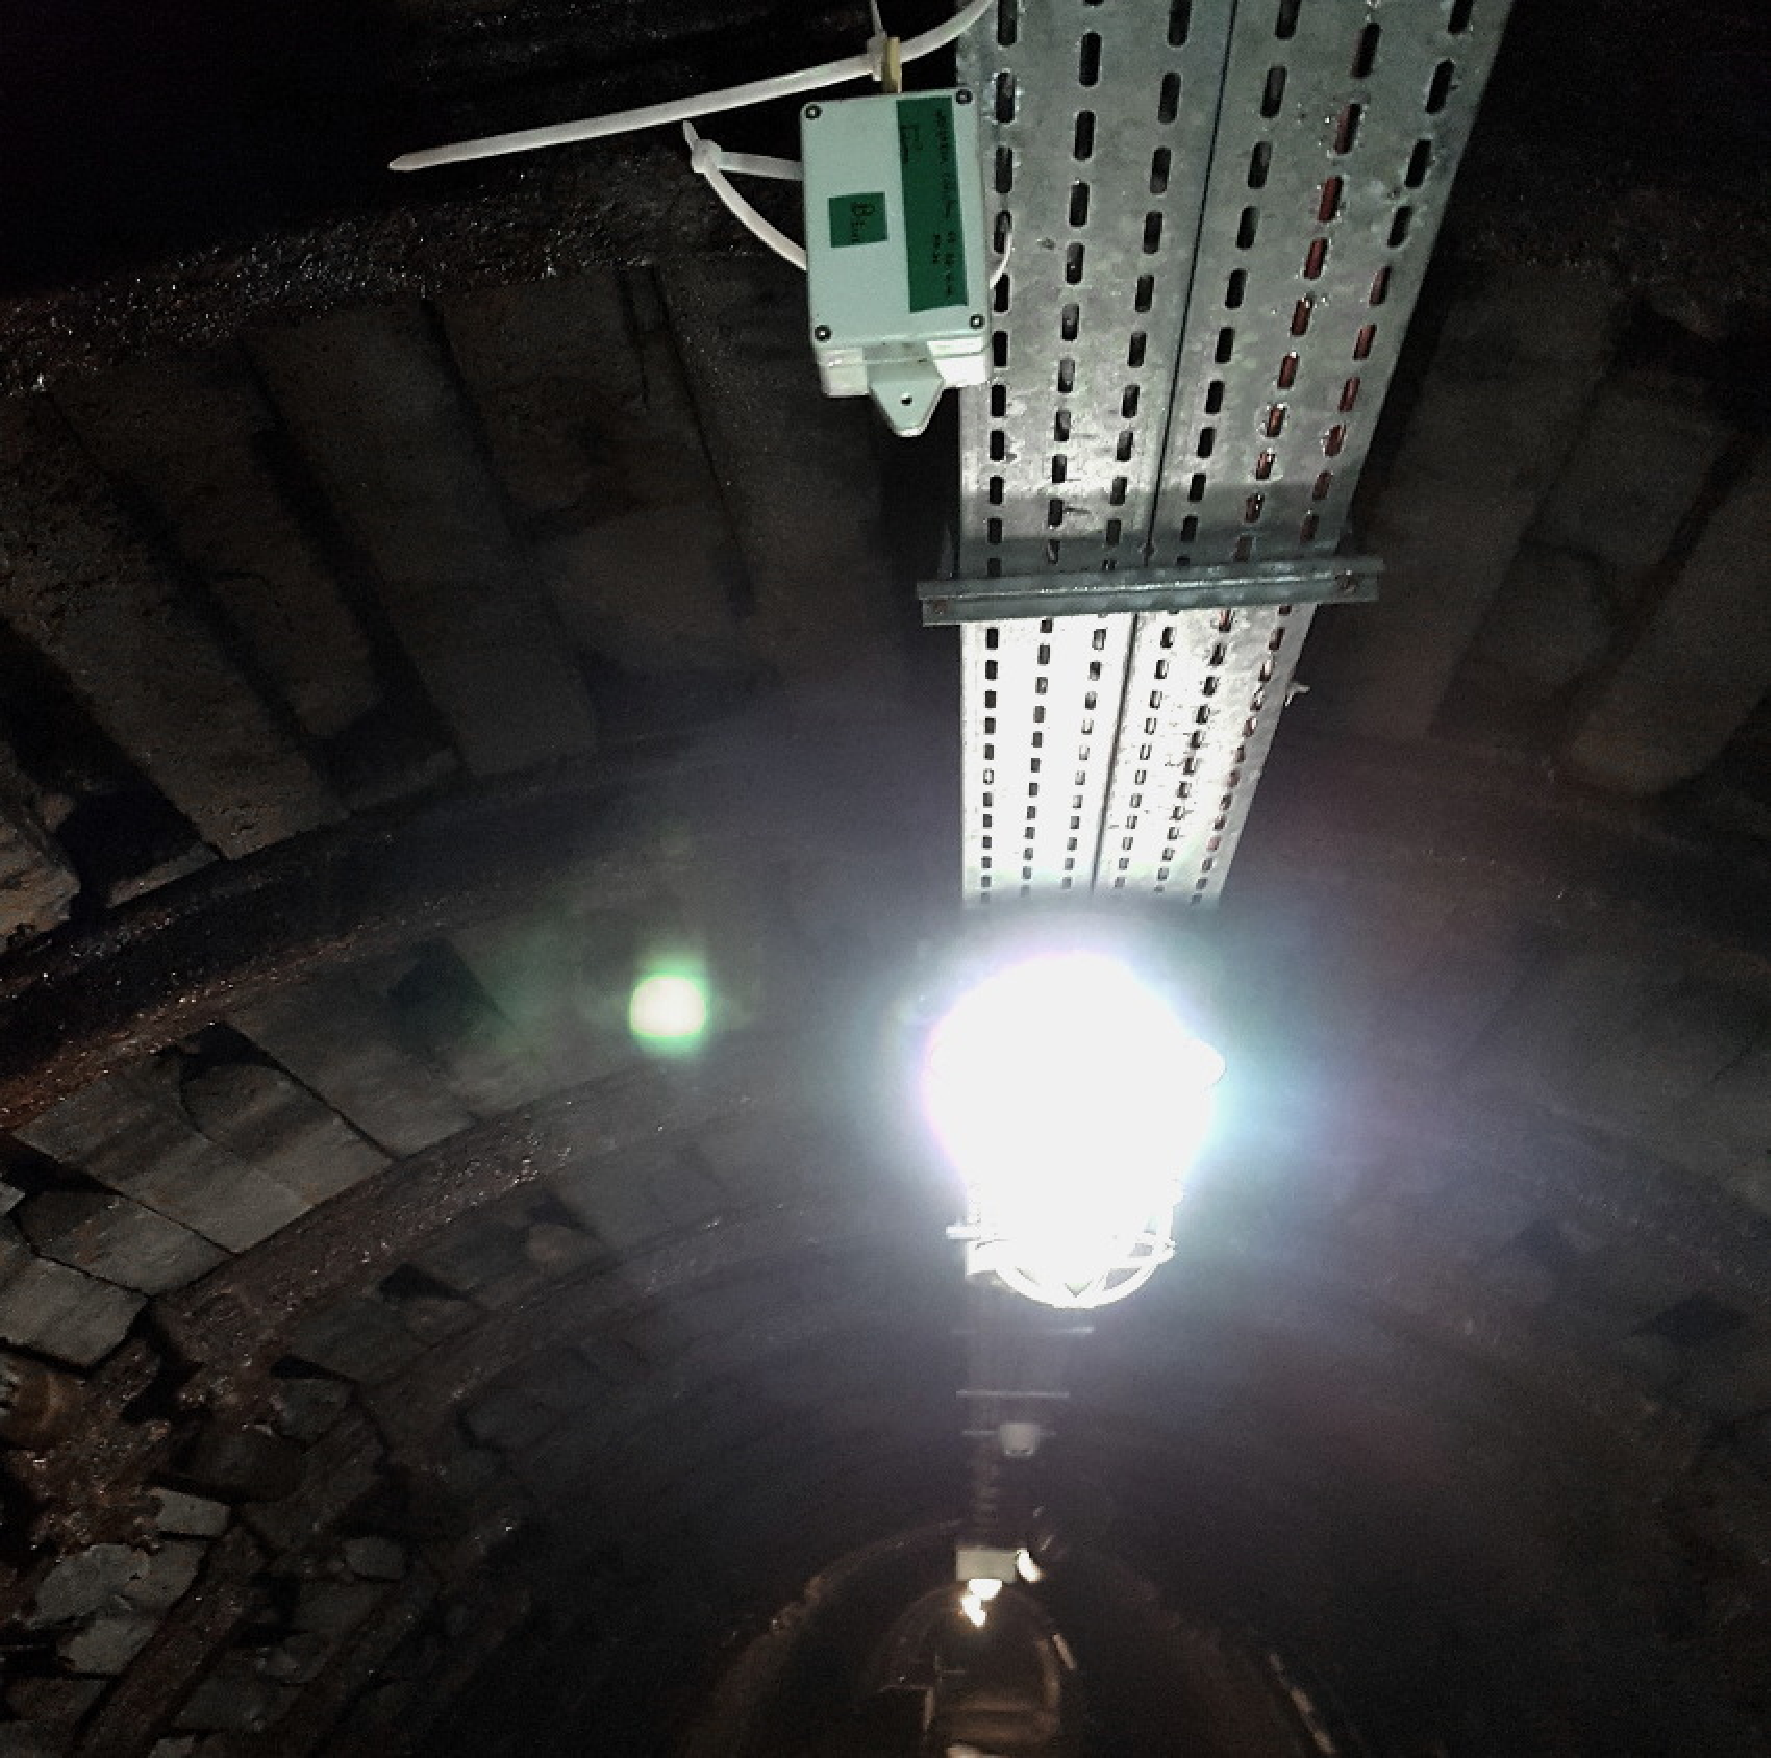
\includegraphics[width=\textwidth, trim={0 1cm 0 0},clip]{pictures/tests_beacon_celing_vertical.pdf}
\caption{Beacon 1 mounterd on a ceiling with vertical antenna direction.}
\label{fig:tests_beacon_celing_vertical}
\end{minipage}
\end{figure}


In order to check what is the signal range of a single beacon device, there was performed a test in which there was taken a series of recived signal measures at given distances from the signal source. There were selected two transmitter power settings for the test: $4 dBm$ which is the higher transmitter power setting and $-16 dBm$ which was taken experimentally. Distances were located at 0, 1, 2, 3, 4, 5, 6, 7, 8, 9, 10, 12,5, 15, 20, 25, 30, 35, 40, 45, 50, 60, 70, 80, 90 meters in case of $4 dBm$ setting and at 0, 1, 2, 3, 4, 6, 8, 10, 12,5, 15, 20, 25, 35 meters in case of $-16 dBm$ setting. During the test there was used "B1" beacon mounted on the ceiling vertically. Figure \ref{fig:tests_case1_attenuation} presents results of this tests.

\begin{figure}[!htbp]
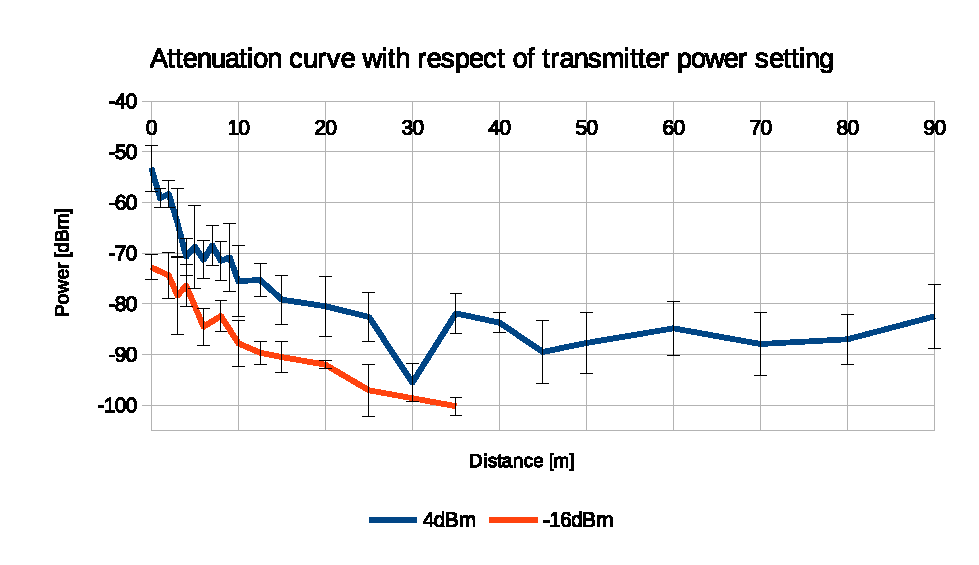
\includegraphics[width=\textwidth, keepaspectratio]{pictures/tests_case1_attenuation}
\centering
\caption{Attenuation curve for $4 dBm$ and $-16 dBm$ trasmitter power.}
\label{fig:tests_case1_attenuation}
\end{figure}

Range of a beacon with the highest power setting available exceeds available space in a corridor, that is why data ends for $4 dBm$ ends at $90 m$. Received signal strengths measured on distances larger than $20m$ from the source of the signal are getting stabilized while strengths mesured closer than $20m$ from the signal source are falling significantly. Measures taken between $20m$ -- $90m$ from signal source are between $-80 dBm$ and $-90 dBm$, while the drop on the first $5m$ from the signal source is about $15 dBm$. What is an interesing is that received signal strength values were not decreasing on distances between $50m$ and $90m$. There was also observed that signal strengths get stabilized on larger distances what was depicted on figure \ref{fig:tests_case1_fluctuations_over_time_std_dev} expressing standard deviation of received signals, as well on figure \ref{fig:tests_case1_fluctuations_over_time} where can be observed the cource of the received signal strength values. Observation matches with the observations about the \textit{log-distance path loss model}.

It is assumed that the solution should be suited for three possible smartphone orientations: smartphone handled in front of the user (vertivally and horizontally) and smartphone kept in the pocket. Figure \ref{fig:tests_case2_smartphone_in_pocket_tx_power} presents results of a dynamic, continous test that consisted of three phases:
\begin{itemize}
	\item measure received signal strength for $5 s$ directly under the transmitter,
	\item walk $5 m$ away,
	\item measure signal for $5 s$ on $5 m$ distance from signal source.
\end{itemize}

 Test was performed 4 times, each for different transmitter power values: $-12dBm$, $-16dBm$, $-20dBm$ and $-30dBm$. Beacon was placed vertically on the ceiling.

\begin{figure}[!htbp]
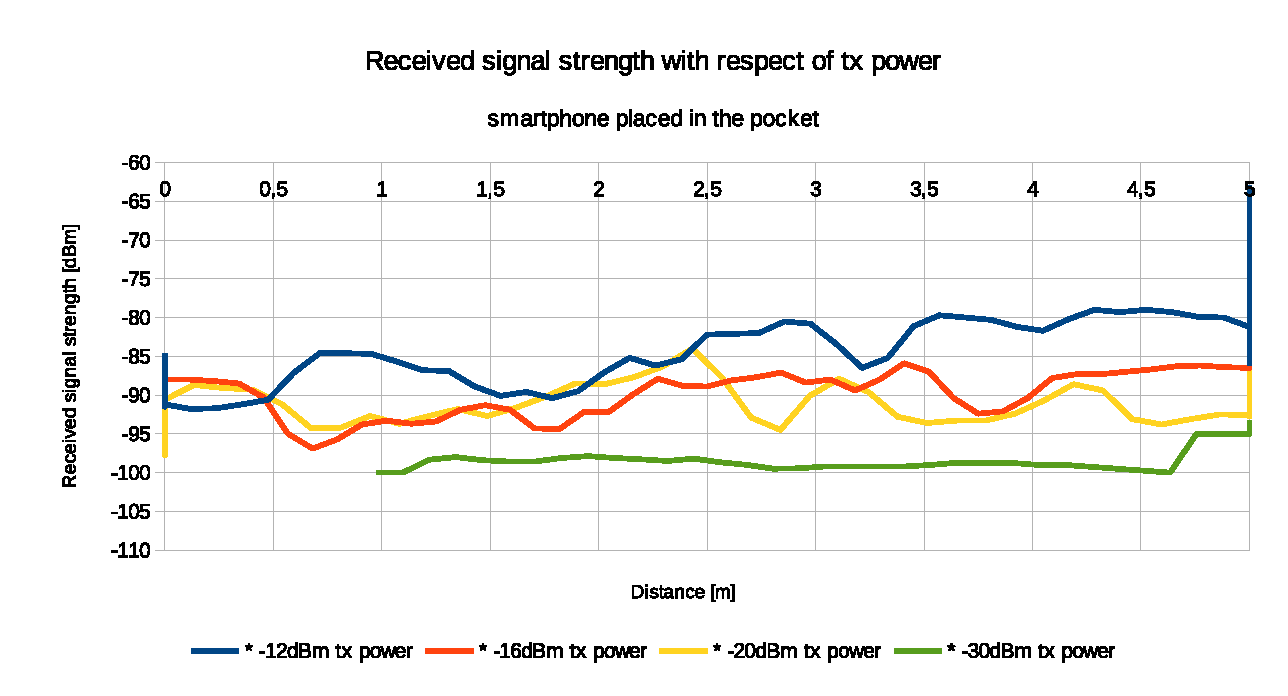
\includegraphics[width=\textwidth, keepaspectratio]{pictures/tests_case2_smartphone_in_pocket_tx_power}
\centering
\caption{Received signal strength values measured by the smartphone kept in the pocket with respect of the trasmitter power and the distance from the signal source.}
\label{fig:tests_case2_smartphone_in_pocket_tx_power}
\end{figure}

Singal strenghts received by the smartphone kept in the pocket are same or even lower at $0m$ distance (smartphone is directly under the beacon) than measured $5m$ away from signal source. Difference is not significant -- in case of $-16dBm$ and $-20dBm$ transmiting power settings, received signal strength values remains the same for the whole test ($\pm 3dBm$). In case of $-12dBm$ transmitter power setting there was observed that received signal got stronger on a $5m$ distance than just bellow the transmitter ($10\pm4 dBm$ change). Received signal strengths of the beacon with $-30dBm$ transmission power setting were low -- signals received in smaller distance than $1m$ from the signal source were ommited, rest were at the border of a noise level. That is why setting $-30dBm$ was rejected as one that provides so week signal, that in case of smartphone kept in the pocket can be filtered out as a noise.

In latter test there were compared smartphone orientations in context of thier influence on the received signal strength value. As it is assumed that the crucial distance for the positioning system, that will allow for accuracy at least equal to the distance between beacons, tests were performed directly under the beacon. Beacon was placed on the ceiling with vertical anetenna direction. Test was a static test where at least 25 probes of the signal strength were taken at the same place. There were tested three values of the transmitter power in order to see if the transmitter power impacts on the all of smartphone orientations equaly. Setting of $-30dBm$ transmitter power was ommited in the evaluation. Results are presented on figure \ref{fig:tests_case3_rssi_vs_smartphone_orientation}.

\begin{figure}[!htbp]
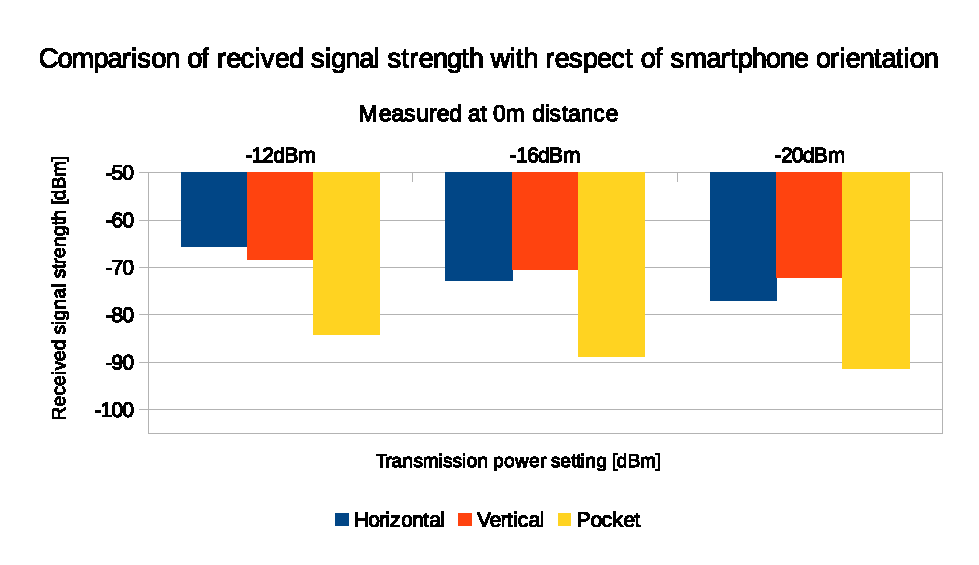
\includegraphics[width=\textwidth, keepaspectratio]{pictures/tests_case3_rssi_vs_smartphone_orientation}
\centering
\caption{Received signal strength measured just under the beacon device mounted on the ceiling in verical orientation. Tested three transmitter power values: $-12dBm$, $-16dBm$ and $-20dBm$ and the three smartphone orientations: vertical, horizontal and kept in the pocket.}
\label{fig:tests_case3_rssi_vs_smartphone_orientation}
\end{figure}

Ideally, change of the transmission power expressed in $dBm$ should cause the same chagne in the received signal strength. That was not observed on the results of performed experiment. Change of $4 dBm$ and $8 dBm$ caused following change in observed signal strengths per smartphone orienations:
\begin{itemize}
	\item horizontally: $7.3\pm2.4 dBm$ and $11.3\pm5.1 dBm$,
	\item vertically: $2\pm4 dBm$ and $8.5\pm5.1 dBm$,
	\item kept in the pocket: $4.5\pm4.8 dBm$ and $7.1\pm3 dBm$.
\end{itemize}

Received signal strengths obtained by the smartphone in horizontal and vertical orientation differs by $2 dBm$ -- $4 dBm$ while standard deviations taken from the set of probes are about $2.5 dBm$ -- $5 dBm$. It means that in this test setup, horizontal and vertical orientations does not impact on the signal in an observable way. Fluctuations as well as obtained RSS value are on the same level. Significant difference is between horizontal or vertical orientation and the placement in the pocket. In all cases received signal strength was about $18\pm2 dBm$ lower. It means that there is need to ensure such setup of the wireless reference point installation that will ensure such transmission power that allow for correct identification of the beacon with some safety factor, even the receiver is in the pocket -- so reflecting additional $18dBm$ needed for this placement. Such safety factor is determined as a lowest acceptable value for the positioning system -- every signal with a lower value is treated as a noise.

Another factor that influence radio frequency transmission is a presence of obstacles between transmitter and receiver. Situation where radio waves that can directly come from the signal source to the receiver without diffractions, in direct path, is called line-of-sight propagation. During the test session there was taken two types of obscuration taken into consideration: obscuration that results from the shape of the tunnel and user obscuration, when the user is in between the smartphone and the beacon. The first case is ilustrated on the figure \ref{fig:tests_case4_los}.

\begin{figure}[!htbp]
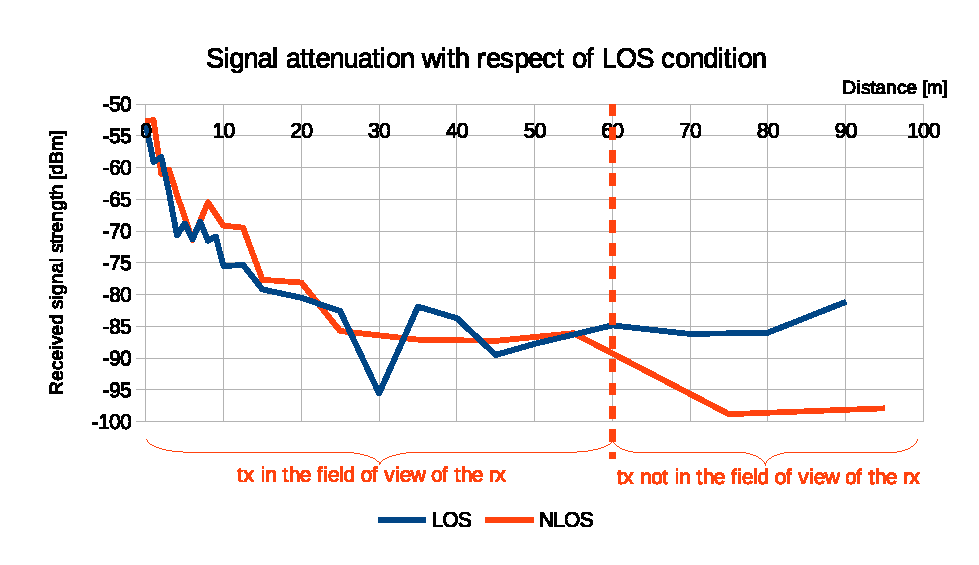
\includegraphics[width=\textwidth, keepaspectratio]{pictures/tests_case4_los}
\centering
\caption{Attenuation curve based on received signal strenght measured at dicrete distances from the signal source. Test taken in corridor which goes up starting from $61.5 m$ from the signal source. Red remarks concerns NLOS propagation and highlights the meter since when steep part of the corridor starts.}
\label{fig:tests_case4_los}
\end{figure}

Test consisted of taking probes of the received signal strengths at discrete distances from the signal source in the "southern" part of the corridor, labeled as \textbf{LOS} and in the "northern" part of the corridor, labeled as \textbf{NLOS} (refer to the test place scheme on the figure \ref{fig:corridor}). Southern part of corridor is flat and there were no obstacles between the beacon and the smartphone during the test. Nothern part of the test place starts to go up at $61.5 m$ from the signal source. Steep grade is about $17\%$ so at $71.5 m$ from the signal source there is no direct path between beacon and the smartphone. Smartphone was oriented horizontally, beacon was mounted vertically on the ceiling.

Despite fluctuation observed at $30 m$ from the signal source in LOS session, the shape of both LOS and NLOS curves of received signal strengths with respect of the distance was comparable until the start of the steep part of the corridor. Then NLOS curve goes down so at $75m$ from the signal source the value of RSS is $-98.8\pm2.1$ which is $18.6dBm$ lower than in case of RSS values observed at similiar distance in LOS case. It means that despite the wave guide effect that was supposed to be observed in case of electromagnetic waves in underground installations \cite{rf_in_tunnel_waveguide_effect}, the influence on the received signal strength is so high that have to be taken into consideration during system planning and installation. This effect can be effectively reduced by limitting the emitted signal power strength and populating the beacon devices.

On the figure \ref{fig:tests_case5_user_shadowing} there are presented received signal strength values obtained within the test of the propagation path obscuration by the user .

\begin{figure}[!htbp]
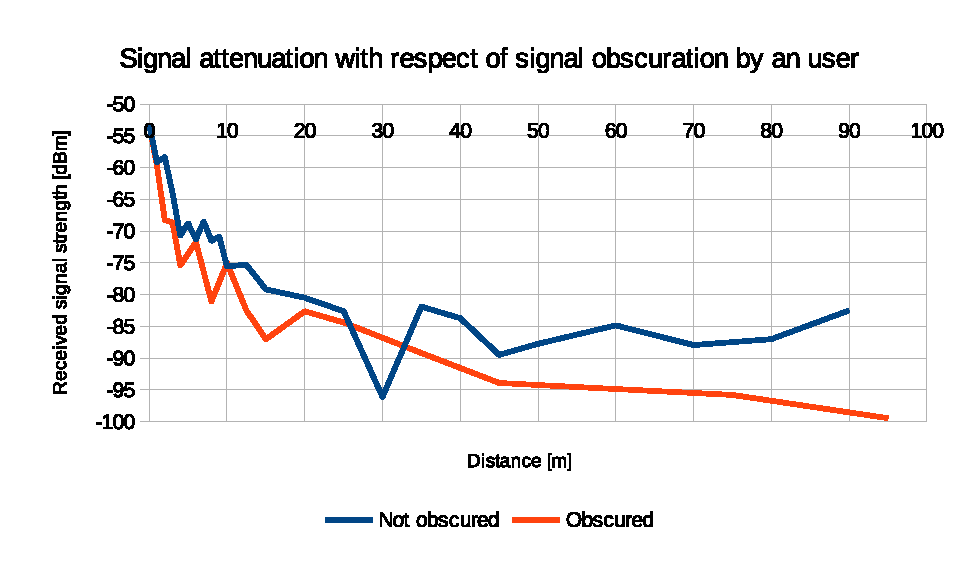
\includegraphics[width=\textwidth, keepaspectratio]{pictures/tests_case5_user_shadowing}
\centering
\caption{Received signal strength with respect of the distance from the signal source and the LOS condition where user is an obstacle on the propagation path.}
\label{fig:tests_case5_user_shadowing}
\end{figure}

Test was performed two times: one session was about taking the measures while user was an obstacle in between the smartphone and the beacon (labeled on chart as "Obscured") and the second session which was about taking the measures while user was not an obstacle (labeled as "Not obscured"). Whole "Obscured" curve is bellow the "Not obscured". The difference between received signal strengths in both conditions is about the same in first $3m$ from the signal source, then is up to $10 dBm$ lower, despite the fluctuations. It means that there is need to reflect the need of additional signal strength required in case of user obscuration into the power setting of the beacons.

The next test, depicted on the figure \ref{fig:tests_case6_tx_placement_and_direction},  is about checking how different beacon placement and its orientation impacts the received signal strength.

\begin{figure}[!htbp]
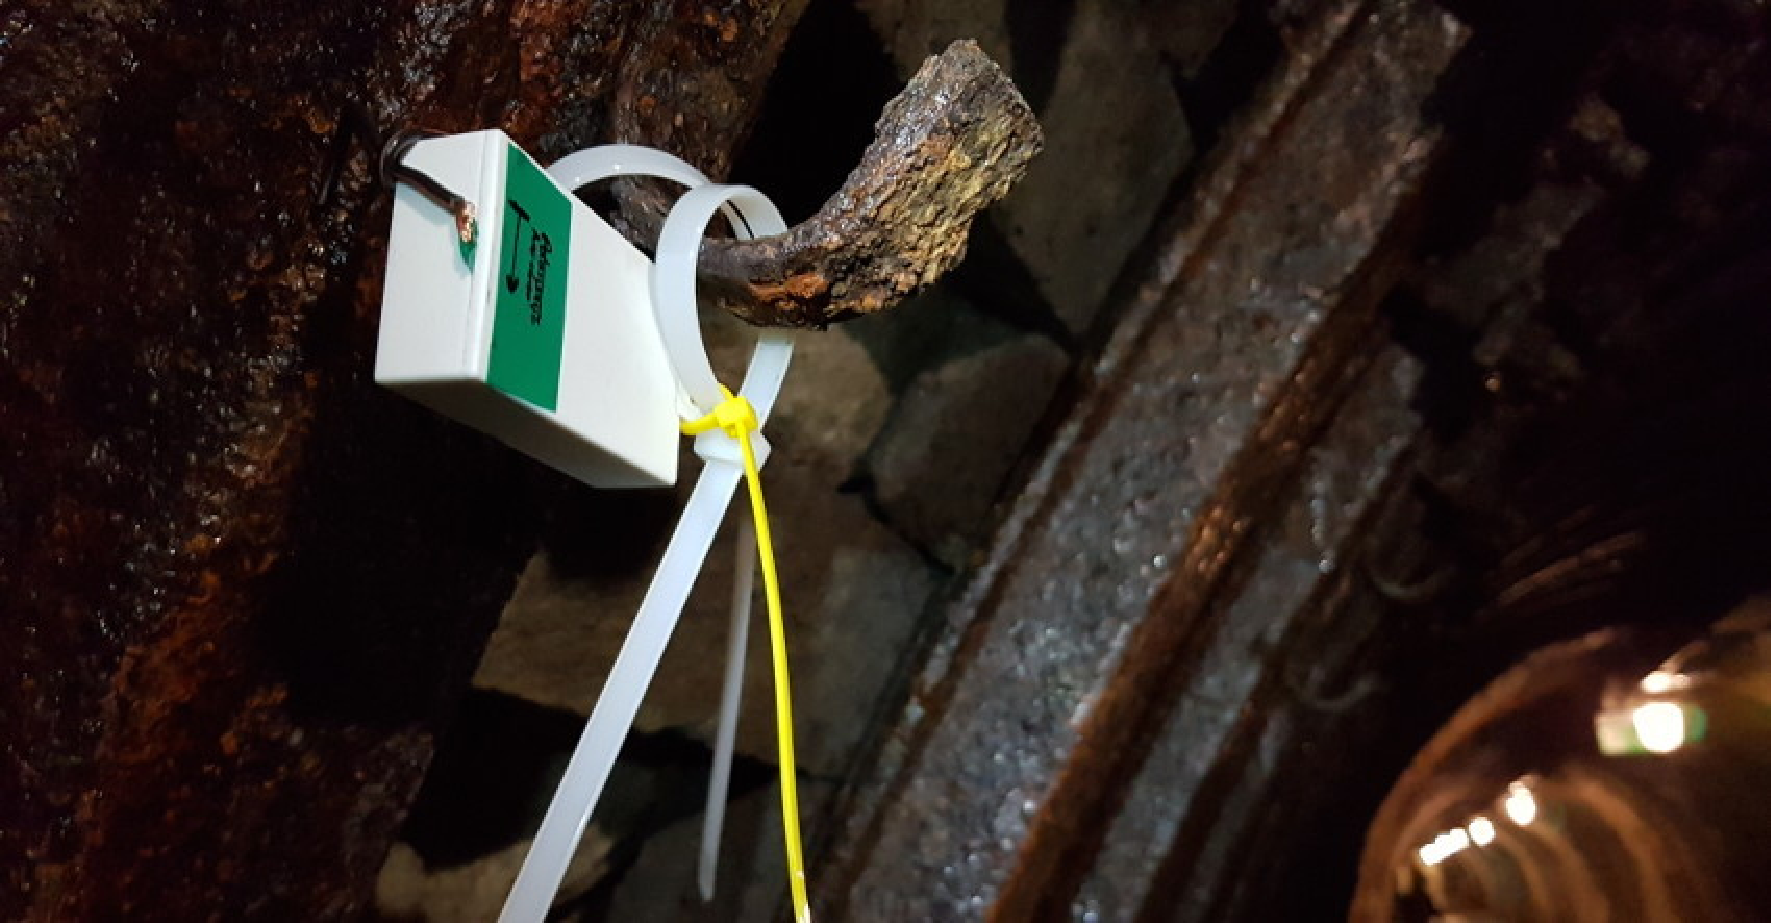
\includegraphics[width=\textwidth, keepaspectratio]{pictures/beacon_wall_vertical.pdf}
\centering
\caption{Beacon B3 mounted on the wall in its vertical orientation.}
\label{fig:beacon_wall_vertical}
\end{figure}

\begin{figure}[!htbp]
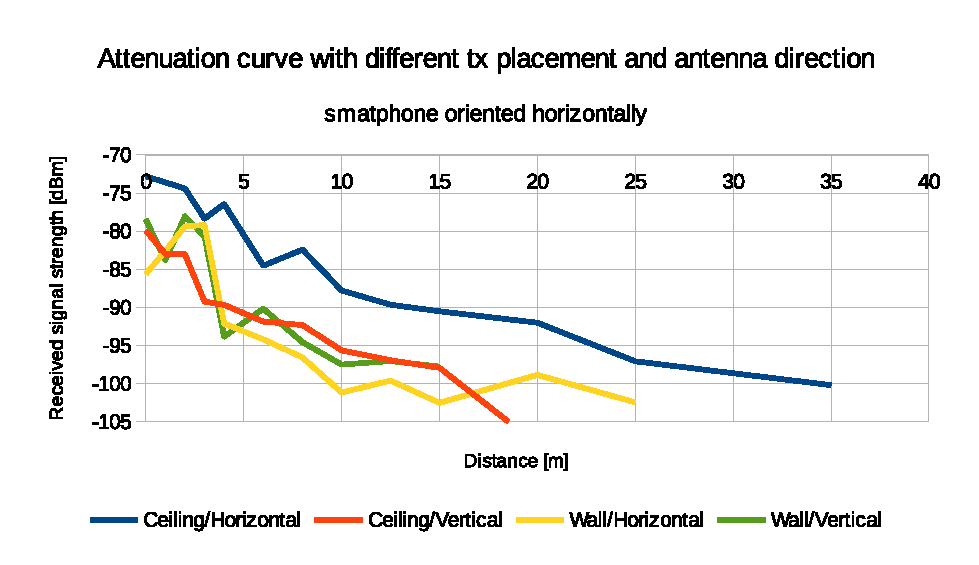
\includegraphics[width=\textwidth, keepaspectratio]{pictures/tests_case6_tx_placement_and_direction}
\centering
\caption{Transmitter position and orientation impact on the received signal strength.}
\label{fig:tests_case6_tx_placement_and_direction}
\end{figure}

The goal of this test was to deduce the best mounting place and orientation of the beacon inside the underground corridor. There were taken into account four possibilities: placement on the ceiling, placement on the wall, with vertical and horizontal antenna directions. On figure \ref{fig:beacon_wall_vertical} there is presented mounting point on the wall. The test was a static one, when probes were taken at discrete distances from the signal source. For test purposes transmitter power got reduced to value of $-16dBm$. Smartphone was oriented horizontally.

The biggest received signal strength values were obtained with the beacon mounted on the ceiling in horizontal antenna direction. Signal strengths were at least $7dBm$ higher for this setting than for any other. There was also observed the biggest signal coverage for this setting -- $35m$. Vertical antenna orienations in both cases of mounting on the ceiling and the wall causes similiar ($\pm5dBm$) RSS values measures, despite the pick on $2m$ from the signal source of beacon mounted on the wall. Both vertical and horizontal orientations of beacon mounted on the wall characterizes with the signal strength pick on $2m$--$3m$ distance from the signal source. Results of the tests points to the fact that beacon placement affects the signal strength as well as the coverage and the part of the fluctuations.

Test of different beacon hardwares was difficult beacause of different electronic solutions being used inside them. Figure \ref{fig:tests_case8_beacons_comparison} presents result of this test.

\begin{figure}[!htbp]
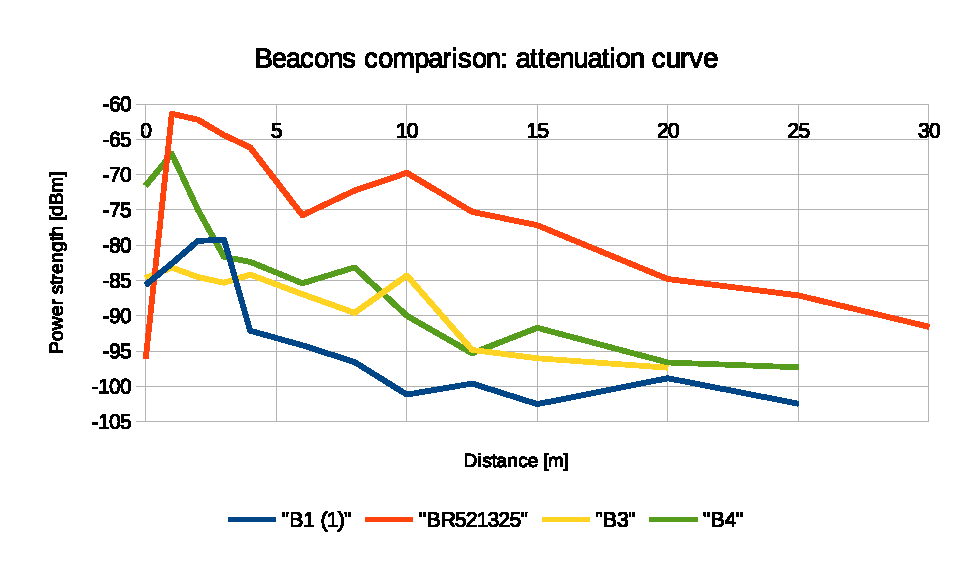
\includegraphics[width=\textwidth, keepaspectratio]{pictures/tests_case8_beacons_comparison}
\centering
\caption{Attenuation curve obtained with use of different beacons and their similiar power setting.}
\label{fig:tests_case8_beacons_comparison}
\end{figure}

There is no standard for creating beacon devices. As many beacons as many hardware solutions for power management, additional sensorics mounted, and the antenna type and installation. In case of beacons that were bought in order to perform tests, each had to be individually configured in order to achive similiar coverage and received signal strengths. That is why value signal strength obtained during the test is not an object of investigation but the curve shape and fluctuations. There were tested beacons B1, B2, B3, B4. Details about the beacons are available in section \ref{sec:tests_criteria_and_assumptions}.

All of the beacons were mounted on the wall, with verical antenna direction. Each of them was tested separately. What is characteristic for that placement is that received signal strength measured at $0 m$ from the beacon is lower than $1$--$2$ meters away. Each measure proves that such rule is true despite different transmitter hardware. There can be also observed that signal strength is the biggest near the source, then drops about $10dBm$ on a distance of $5m$ from the signal source. Situation repeates with smaller aplitudes till the minimum acceptable signal strenght values. In case of beacon B1, B2 and B4 there were observed such values in the close distance to the signal source (about $0m$--$5m$) that significantly differs from those observed in bigger distances. Only B3 beacon emmit it's signal on not disitnguishable power levels within the close range.

The next figure (\ref{fig:tests_case9_smartphone_comparison}) presents results of test with different smartphones being used as receivers of the signal.

\begin{figure}[!htbp]
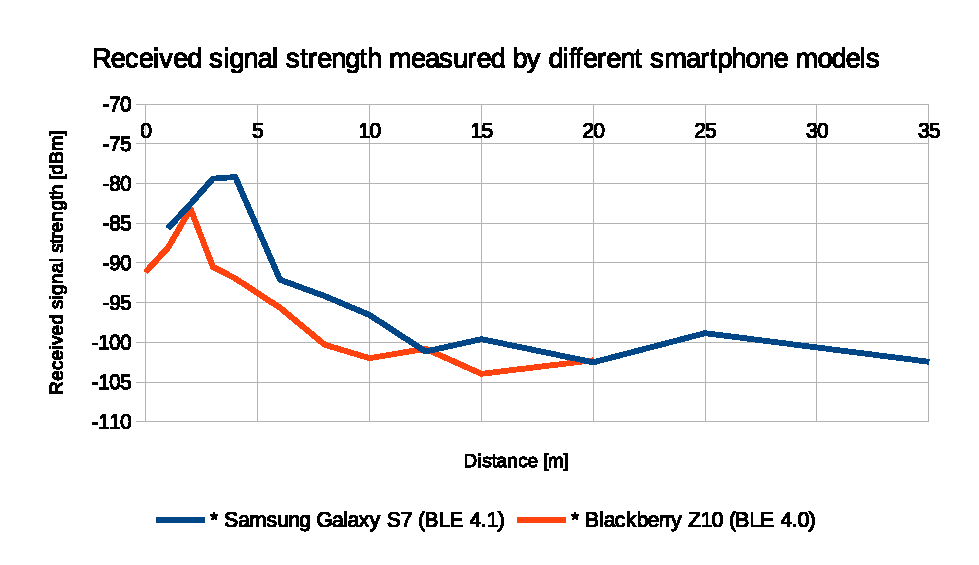
\includegraphics[width=\textwidth, keepaspectratio]{pictures/tests_case9_smartphone_comparison}
\centering
\caption{Comparison of received signal strength values caputered by two different smartphone models: Samsung Galaxy S7 and Blackberry Z10.}
\label{fig:tests_case9_smartphone_comparison}
\end{figure}

For this test there was used beacon B1 mounted vertically on the wall. There were performed measures of the RSS signal taken by two models of smartphones at 0, 1, 2, 3, 4, 6, 8, 10, 12.5, 15, 20, 25, 35 meters from the beacon. Curve shapes for both smartphones are moved with respect to each other by $5dBm$ on $0m$--$4m$ distances. Then the difference is about $2dBm$. Difference may come from the type and the amount material that was used to cover antennas inside the devices. Despite slight differences between signal strength, the receives signal strength pick is distinguishable by both smartphones. Bluetooth standard implemented by two smartphones also do not affect shape of attenuation curve. That means that the solution build on the Bluetooth technology based beacons behaves same for different types of smartphones being used.

% subsection robustness_of_a_received_signal_strenght_measures (end)
\FloatBarrier
\subsection{Real case scenario evaluation} % (fold)
\label{sub:real_case_scenario_evaluation}

Second part of the test session in the underground installation was devoted to check if proposed position fining system based on the wireless reference points (Bluetooth becons) can take received signal strength as a fator determining the distance between the user device and the reference point. Aim of tests was take strength values of signals from beacons during the walk along the tunnel with sample positioning infrastructure and check how the oberved values fits to the proposed positioning solution.

\begin{figure}[!htbp]
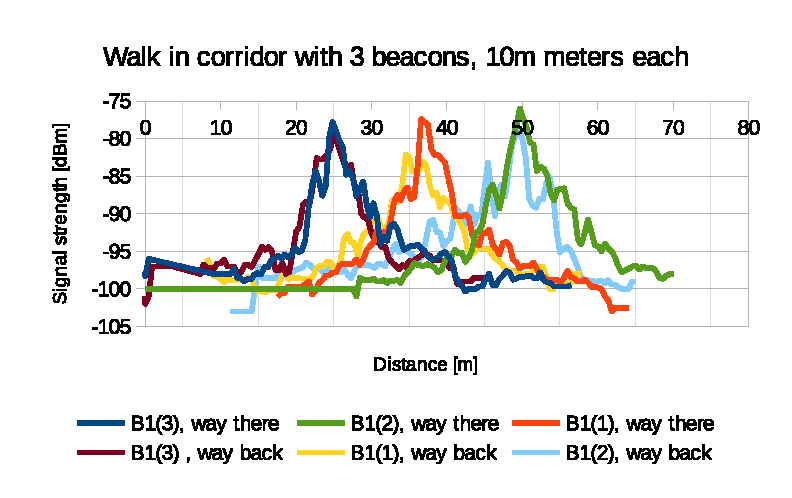
\includegraphics[width=\textwidth, keepaspectratio]{pictures/tests_case10_walk_10m_raw}
\centering
\caption{Signal strengths of the beacons placed $10m$ each, measured during the walk with smartphone hold in hand in it's horizontal orientation.}
\label{fig:tests_case10_walk_10m_raw}
\end{figure}

During tests there was 3 scenarios taken into consideration. One was about position of the smartphone: evalutaion of the signal strength values recorder by the smartphone carried in the pocket and smartphone held by the user in his hand (horizontal orientation). The second scenario consers distance between the reference points. There were evaluated $10m$ and $15m$ distances between the beacons. There were used three B1 beacons with $-16dBm$ power setting placed vertically on the wall. The last scenario was about checking how direction of user movement impacts on the observed signal strength values. That case is a direct extension to the static tests of shadowing direct signal path by the user (see figure \ref{fig:tests_case5_user_shadowing}).

Each test that cover first and the second senario, was performed two times, named as: "way there" and "way back". That is how the third senarios was included into two two first. That way creates the possibility to check if walking direction influence received signal strength. Each test round consisted of three phases: warm up, walk, settle down. Warm up phase was about capturing the signal strength values for $5s$, $20m$ before first beacon. Walk was about making a distance of $70m$ in case of beacons mounted $10m$ each or a distance of $80m$ in case of beacons mounted $15m$ each. Settle down phase ends with $5s$ measurement of signal strength at distance of $20m$ after last beacon mounted on the wall.

Walking pace and speed was not arbitraty set and controlled during test. That is why distances assigned to given values are aproximated under assumption that the pace was contant during the walk. Instead of matching distances to signal strength values picks there was evaluated how signal strenth values changes during the walk.


First test concernes walk with the smartphone hold in hand horizontally and beacons placed in $10m$ distances between each other. Figure \ref{fig:tests_case10_walk_10m_raw} depicts RSS values recorded by the smartphone. Approximate placement of the reference point can be determined because of characterisic picks. There can be also observed that at level of $-95dBm$ signals strength from beacons got sabilized. Because of the fluctuations these signal strength values are not usefull. Beacons emmit their signal with such power level that when the user was just under the second beacon B1(1) (about $35m$ on the chart) he was still received signals from the nearby beacons: B1(3) -- $-95dBm$, B1(2) -- $-97dBm$. It can be observed that in the middle of the distance between nearby beacons, they have similiar power values like in case of B1(3) and B1(1) at $31$ meter: B1(3) -- $-91,6dBm$, B1(1) -- $-91dBm$.


\begin{figure}[!htbp]
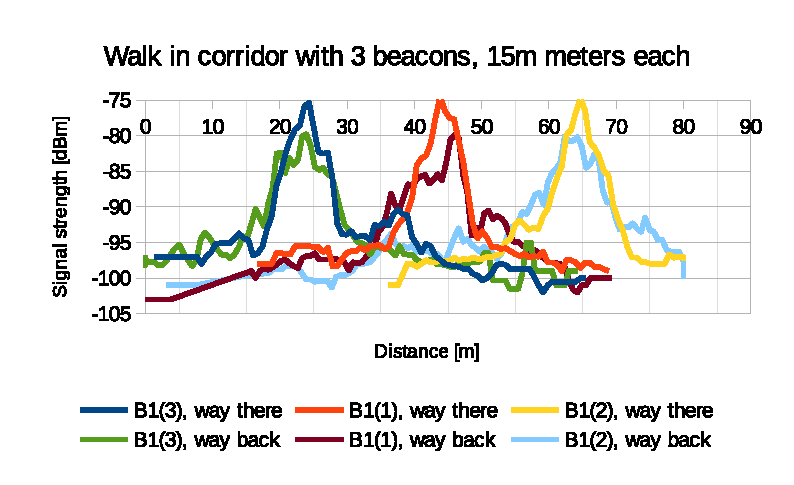
\includegraphics[width=\textwidth, keepaspectratio]{pictures/tests_case10_walk_15m_raw}
\centering
\caption{Attenuation curve with respect of the trasmitter power.}
\label{fig:tests_case10_walk_15m_raw}
\end{figure}

It can be observed that slope of the curve after reaching its peak is slighly smoother than just before the peak. There are are possible two reasons of such results. Values could got smoothed during the signal processing by the hardware or software before value evaluation. It may also mean that the user presence on direct path between beacon and smartphone can ifluence the observed signal strengths.

Figure \ref{fig:tests_case10_walk_15m_raw} presents values obtained during test with beacons placed $15m$ each. Absolute values recorded during the test are similiar to those from previous test. In test with $10m$ gaps, values in peaks were about $-78dBm$ -- $-76dBm$; in test with $15m$ gaps, values in peaks were about $-75dBm$ -- $-74dBm$. Also the RSS values in the middle of distances between two nearby beacons are similiar, about $-95dBm$.

\begin{figure}[!htbp]
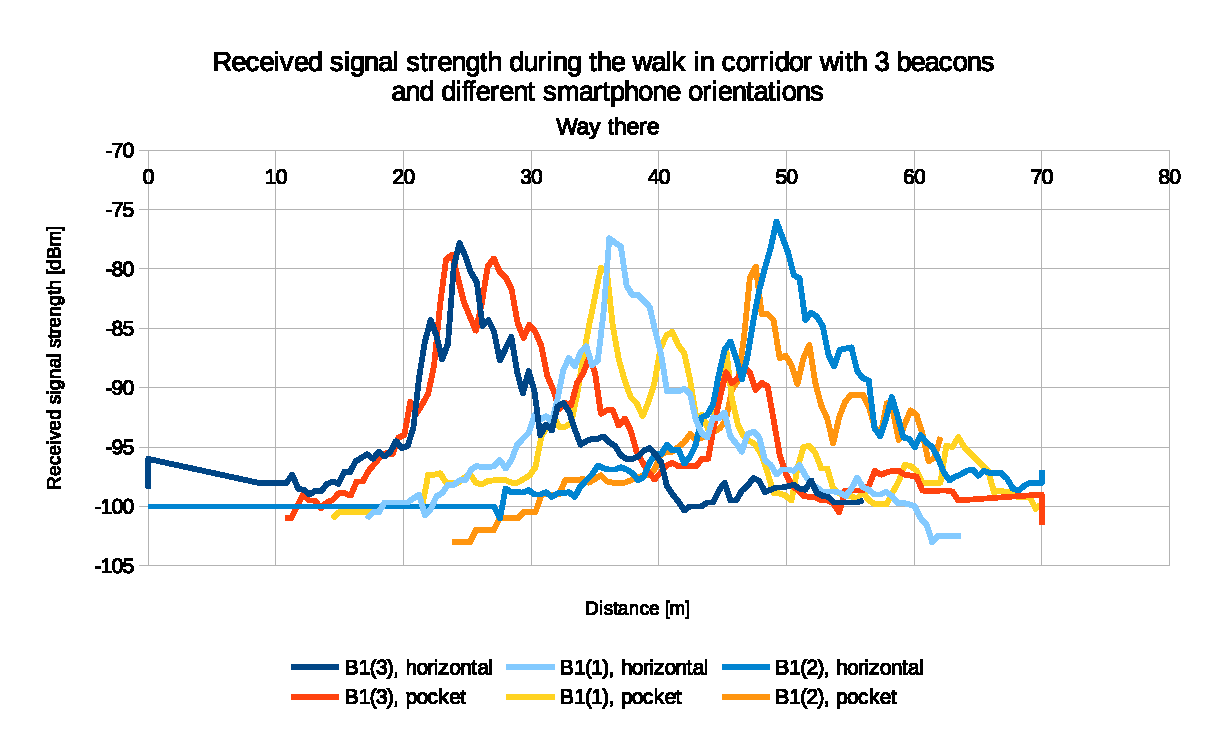
\includegraphics[width=\textwidth, keepaspectratio]{pictures/tests_case11_walk_10m_smartphone_orientation}
\centering
\caption{Attenuation curve of three beacons with respect of the placement of the smartphone.}
\label{fig:tests_case11_walk_10m_smartphone_orientation}
\end{figure}

Figure \ref{fig:tests_case11_walk_10m_smartphone_orientation} presents results of a test where beacons were placed $10m$ each and the smatphone was kept in the pocket. The main difference between signals recorded by smartphone in its horizontal orientation and when it was kept in the pocket is the strong fluctuation near the signal source. It is most visible on meter $35$ and $38$ where yellow cruve of RSS of beacon B1(1) drops from $-79dBm$ to $-92dBm$ and then goes up to $-85dBm$ at $40$ meter.


% subsection real_case_scenario_evaluation (end)
% section tests_of_system_and_basic_algorithm (end)
\FloatBarrier

\section{Application of signal filtering} % (fold)
\label{sec:application_of_signal_filtering}

In order to improve the accuracy of the signal strength based positioning, there was applied low-pass filtering to the measures. Filtering aim is to limit signal strength fluctuations. Figure \ref{fig:tests_case10_walk_10m_low_pass} presents filtered values obtained during dynamic test presented before on figure \ref{fig:tests_case10_walk_10m_raw}.


\begin{figure}[!htbp]
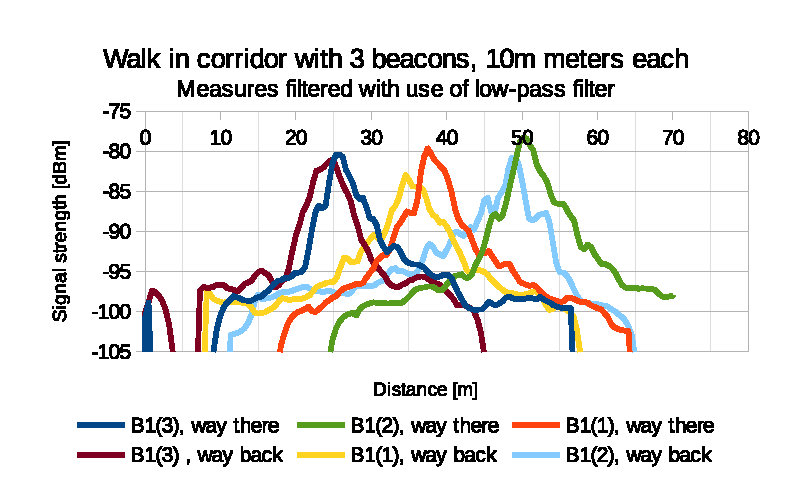
\includegraphics[width=\textwidth, keepaspectratio]{pictures/tests_case10_walk_10m_low_pass}
\centering
\caption{Attenuation curve with respect of the trasmitter power.}
\label{fig:tests_case10_walk_10m_low_pass}
\end{figure}

\begin{figure}[!htbp]
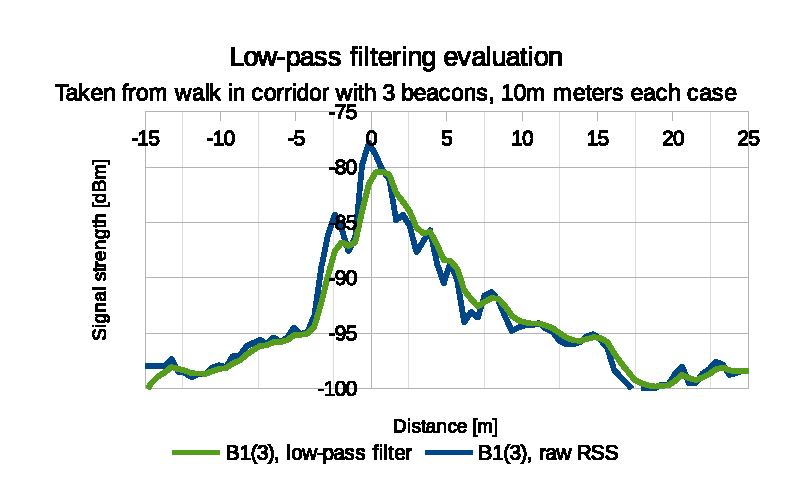
\includegraphics[width=\textwidth,clip]{pictures/tests_case10_b1_3_low_pass}
\caption{Comparison of raw and low-pass filtered RSS values of B1(3) taken from dynamic test with 3 beacons.}
\label{fig:tests_case10_b1_3_low_pass}
\end{figure}
\begin{figure}[!htbp]
 % trim={<left> <lower> <right> <upper>}
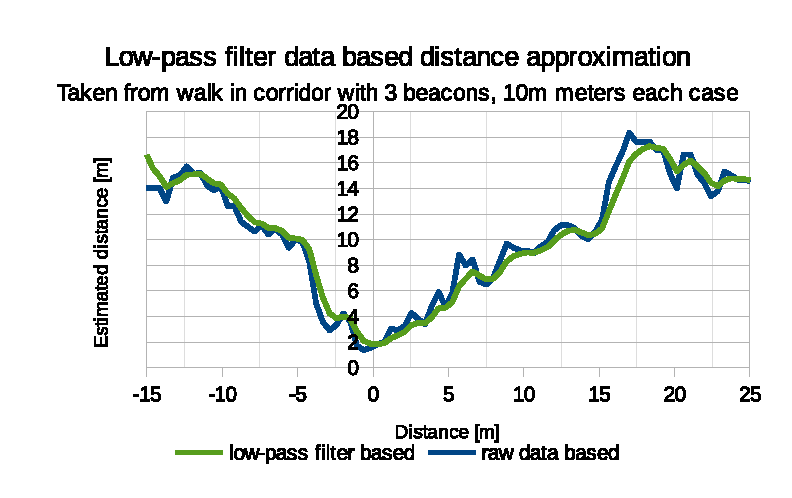
\includegraphics[width=\textwidth,clip]{pictures/tests_case10_b1_3_low_pass_dist_model}
\caption{Comparison of distance model approximation based on raw and low-pass filtered RSS values.}
\label{fig:tests_case10_b1_3_low_pass_dist_model}
\end{figure}


Low-pass filter does not smoothed the signal in a way that no fluctuactions can be observed but it limits their amplitude. For example drop at $23m$ of a RSS from beacon B1(3) got reduced from $-2dBm$ to $-0.3dBm$.

Drawback of such data filtering is that it introduces some delay to dynamically changing values. For example: RSS value pick of B1(3) beacon in not filtered data (fig. \ref{fig:tests_case10_b1_3_low_pass}) was observed at $0m$ while pick on filtered data was observed $1m$ further ($3$ RSS probes later), assuming $1.6\frac{km}{h}$ test device speed and $1Hz$ frequency of RSS probing. Problem may be overcome by increasing probing frequency but decreasing the beacon battery life.

Figure \ref{fig:tests_case10_b1_3_low_pass_dist_model} presents how low-pass filter affects distance aproximations of \textit{log-distance path loss model}. Model was adjusted to match lower transmitter signal power ($-16dBm$ used during the test). Filtering does not improve or decrease accuracy of the model, just smooth resulting values.

Low-pass filtering does not solve the problem of RSS values fluctuations but it is a good solution to limit effects of a random, highly differenet values of RSS happening during the measurement session.

% section tests_of_extended_algorithm (end)
\FloatBarrier

\section{Mobile application} % (fold)
\label{sec:mobile_application}

% section mobile_application (end)

\section{Tests summary} % (fold)
\label{sec:tests_summary}
\begin{itemize}
	\item State if some factors have impact on signal quality
	\item State if some factors have impact on position finding
\end{itemize}

% section tests_summary (end)
\end{document}
